\documentclass{book}
\usepackage[a4paper,top=2.5cm,bottom=2.5cm,left=2.5cm,right=2.5cm]{geometry}
\usepackage{makeidx}
\usepackage{natbib}
\usepackage{graphicx}
\usepackage{multicol}
\usepackage{float}
\usepackage{listings}
\usepackage{color}
\usepackage{ifthen}
\usepackage[table]{xcolor}
\usepackage{textcomp}
\usepackage{alltt}
\usepackage{ifpdf}
\ifpdf
\usepackage[pdftex,
            pagebackref=true,
            colorlinks=true,
            linkcolor=blue,
            unicode
           ]{hyperref}
\else
\usepackage[ps2pdf,
            pagebackref=true,
            colorlinks=true,
            linkcolor=blue,
            unicode
           ]{hyperref}
\usepackage{pspicture}
\fi
\usepackage[utf8]{inputenc}
\usepackage{mathptmx}
\usepackage[scaled=.90]{helvet}
\usepackage{courier}
\usepackage{sectsty}
\usepackage{amssymb}
\usepackage[titles]{tocloft}
\usepackage{doxygen}
\lstset{language=C++,inputencoding=utf8,basicstyle=\footnotesize,breaklines=true,breakatwhitespace=true,tabsize=4,numbers=left }
\makeindex
\setcounter{tocdepth}{3}
\renewcommand{\footrulewidth}{0.4pt}
\renewcommand{\familydefault}{\sfdefault}
\hfuzz=15pt
\setlength{\emergencystretch}{15pt}
\hbadness=750
\tolerance=750
\begin{document}
\hypersetup{pageanchor=false,citecolor=blue}
\begin{titlepage}
\vspace*{7cm}
\begin{center}
{\Large S\-A104\-X }\\
\vspace*{1cm}
{\large Generated by Doxygen 1.8.3.1}\\
\vspace*{0.5cm}
{\small Mon Mar 25 2013 11:20:34}\\
\end{center}
\end{titlepage}
\clearemptydoublepage
\pagenumbering{roman}
\tableofcontents
\clearemptydoublepage
\pagenumbering{arabic}
\hypersetup{pageanchor=true,citecolor=blue}
\chapter{sa104x-\/kexjobb}
\label{md_README}
\hypertarget{md_README}{}
Implementation of a verifier for the Verificatum Mix-\/net

\subsection*{Requirements}


\begin{DoxyItemize}
\item Open\-S\-S\-L
\item G\-M\-P
\item Rapid\-X\-M\-L 
\end{DoxyItemize}
\chapter{Hierarchical Index}
\section{Class Hierarchy}
This inheritance list is sorted roughly, but not completely, alphabetically\-:\begin{DoxyCompactList}
\item \contentsline{section}{Base\-Node}{\pageref{class_base_node}}{}
\begin{DoxyCompactList}
\item \contentsline{section}{Base\-Leaf}{\pageref{class_base_leaf}}{}
\begin{DoxyCompactList}
\item \contentsline{section}{Data\-Leaf}{\pageref{class_data_leaf}}{}
\item \contentsline{section}{Int\-Leaf}{\pageref{class_int_leaf}}{}
\end{DoxyCompactList}
\item \contentsline{section}{Node}{\pageref{class_node}}{}
\end{DoxyCompactList}
\item \contentsline{section}{P\-R\-G}{\pageref{class_p_r_g}}{}
\item \contentsline{section}{proof\-Struct}{\pageref{structproof_struct}}{}
\item \contentsline{section}{R\-O}{\pageref{class_r_o}}{}
\end{DoxyCompactList}

\chapter{Class Index}
\section{Class List}
Here are the classes, structs, unions and interfaces with brief descriptions\-:\begin{DoxyCompactList}
\item\contentsline{section}{\hyperlink{class_base_leaf}{Base\-Leaf} }{\pageref{class_base_leaf}}{}
\item\contentsline{section}{\hyperlink{class_base_node}{Base\-Node} }{\pageref{class_base_node}}{}
\item\contentsline{section}{\hyperlink{class_data_leaf}{Data\-Leaf} }{\pageref{class_data_leaf}}{}
\item\contentsline{section}{\hyperlink{class_int_leaf}{Int\-Leaf} }{\pageref{class_int_leaf}}{}
\item\contentsline{section}{\hyperlink{class_node}{Node} }{\pageref{class_node}}{}
\item\contentsline{section}{\hyperlink{class_p_r_g}{P\-R\-G} }{\pageref{class_p_r_g}}{}
\item\contentsline{section}{\hyperlink{structproof_struct}{proof\-Struct} }{\pageref{structproof_struct}}{}
\item\contentsline{section}{\hyperlink{class_r_o}{R\-O} }{\pageref{class_r_o}}{}
\end{DoxyCompactList}

\chapter{File Index}
\section{File List}
Here is a list of all files with brief descriptions\-:\begin{DoxyCompactList}
\item\contentsline{section}{Arithmetic/\hyperlink{_base_leaf_8cpp}{Base\-Leaf.\-cpp} }{\pageref{_base_leaf_8cpp}}{}
\item\contentsline{section}{Arithmetic/\hyperlink{_base_leaf_8h}{Base\-Leaf.\-h} }{\pageref{_base_leaf_8h}}{}
\item\contentsline{section}{Arithmetic/\hyperlink{_base_node_8cpp}{Base\-Node.\-cpp} }{\pageref{_base_node_8cpp}}{}
\item\contentsline{section}{Arithmetic/\hyperlink{_base_node_8h}{Base\-Node.\-h} }{\pageref{_base_node_8h}}{}
\item\contentsline{section}{Arithmetic/\hyperlink{_data_leaf_8cpp}{Data\-Leaf.\-cpp} }{\pageref{_data_leaf_8cpp}}{}
\item\contentsline{section}{Arithmetic/\hyperlink{_data_leaf_8h}{Data\-Leaf.\-h} }{\pageref{_data_leaf_8h}}{}
\item\contentsline{section}{Arithmetic/\hyperlink{_int_leaf_8cpp}{Int\-Leaf.\-cpp} }{\pageref{_int_leaf_8cpp}}{}
\item\contentsline{section}{Arithmetic/\hyperlink{_int_leaf_8h}{Int\-Leaf.\-h} }{\pageref{_int_leaf_8h}}{}
\item\contentsline{section}{Arithmetic/\hyperlink{_node_8cpp}{Node.\-cpp} }{\pageref{_node_8cpp}}{}
\item\contentsline{section}{Arithmetic/\hyperlink{_node_8h}{Node.\-h} }{\pageref{_node_8h}}{}
\item\contentsline{section}{Arithmetic/\hyperlink{types_8h}{types.\-h} }{\pageref{types_8h}}{}
\item\contentsline{section}{Crypto/\hyperlink{_el_gamal_8cpp}{El\-Gamal.\-cpp} }{\pageref{_el_gamal_8cpp}}{}
\item\contentsline{section}{Crypto/\hyperlink{_el_gamal_8h}{El\-Gamal.\-h} }{\pageref{_el_gamal_8h}}{}
\item\contentsline{section}{Crypto/\hyperlink{_h___s_h_a_8cpp}{H\-\_\-\-S\-H\-A.\-cpp} }{\pageref{_h___s_h_a_8cpp}}{}
\item\contentsline{section}{Crypto/\hyperlink{_h___s_h_a_8h}{H\-\_\-\-S\-H\-A.\-h} }{\pageref{_h___s_h_a_8h}}{}
\item\contentsline{section}{Crypto/\hyperlink{_p_r_g_8cpp}{P\-R\-G.\-cpp} }{\pageref{_p_r_g_8cpp}}{}
\item\contentsline{section}{Crypto/\hyperlink{_p_r_g_8h}{P\-R\-G.\-h} }{\pageref{_p_r_g_8h}}{}
\item\contentsline{section}{Crypto/\hyperlink{_random_array_8cpp}{Random\-Array.\-cpp} }{\pageref{_random_array_8cpp}}{}
\item\contentsline{section}{Crypto/\hyperlink{_random_array_8h}{Random\-Array.\-h} }{\pageref{_random_array_8h}}{}
\item\contentsline{section}{Crypto/\hyperlink{_r_o_8cpp}{R\-O.\-cpp} }{\pageref{_r_o_8cpp}}{}
\item\contentsline{section}{Crypto/\hyperlink{_r_o_8h}{R\-O.\-h} }{\pageref{_r_o_8h}}{}
\item\contentsline{section}{Tests/\hyperlink{_byte_tree_tests_8cpp}{Byte\-Tree\-Tests.\-cpp} }{\pageref{_byte_tree_tests_8cpp}}{}
\item\contentsline{section}{Tests/\hyperlink{_int_leaf_arithmetics_tests_8cpp}{Int\-Leaf\-Arithmetics\-Tests.\-cpp} }{\pageref{_int_leaf_arithmetics_tests_8cpp}}{}
\item\contentsline{section}{Tests/\hyperlink{_node_arithmetics_tests_8cpp}{Node\-Arithmetics\-Tests.\-cpp} }{\pageref{_node_arithmetics_tests_8cpp}}{}
\item\contentsline{section}{Tests/\hyperlink{_node_data_init_tests_8cpp}{Node\-Data\-Init\-Tests.\-cpp} }{\pageref{_node_data_init_tests_8cpp}}{}
\item\contentsline{section}{Tests/\hyperlink{_node_to_string_tests_8cpp}{Node\-To\-String\-Tests.\-cpp} }{\pageref{_node_to_string_tests_8cpp}}{}
\item\contentsline{section}{Tests/\hyperlink{_p_r_g_tests_8cpp}{P\-R\-G\-Tests.\-cpp} }{\pageref{_p_r_g_tests_8cpp}}{}
\item\contentsline{section}{Tests/\hyperlink{_test_runner_8cpp}{Test\-Runner.\-cpp} }{\pageref{_test_runner_8cpp}}{}
\item\contentsline{section}{Verifier/\hyperlink{_decryption_factors_verifier_8cpp}{Decryption\-Factors\-Verifier.\-cpp} }{\pageref{_decryption_factors_verifier_8cpp}}{}
\item\contentsline{section}{Verifier/\hyperlink{_decryption_factors_verifier_8h}{Decryption\-Factors\-Verifier.\-h} }{\pageref{_decryption_factors_verifier_8h}}{}
\item\contentsline{section}{Verifier/\hyperlink{_decryption_verifier_8cpp}{Decryption\-Verifier.\-cpp} }{\pageref{_decryption_verifier_8cpp}}{}
\item\contentsline{section}{Verifier/\hyperlink{_decryption_verifier_8h}{Decryption\-Verifier.\-h} }{\pageref{_decryption_verifier_8h}}{}
\item\contentsline{section}{Verifier/\hyperlink{_file_names_8h}{File\-Names.\-h} }{\pageref{_file_names_8h}}{}
\item\contentsline{section}{Verifier/\hyperlink{_key_verifier_8cpp}{Key\-Verifier.\-cpp} }{\pageref{_key_verifier_8cpp}}{}
\item\contentsline{section}{Verifier/\hyperlink{_key_verifier_8h}{Key\-Verifier.\-h} }{\pageref{_key_verifier_8h}}{}
\item\contentsline{section}{Verifier/\hyperlink{main_8cpp}{main.\-cpp} }{\pageref{main_8cpp}}{}
\item\contentsline{section}{Verifier/\hyperlink{_proof_of_shuffle_8cpp}{Proof\-Of\-Shuffle.\-cpp} }{\pageref{_proof_of_shuffle_8cpp}}{}
\item\contentsline{section}{Verifier/\hyperlink{_proof_of_shuffle_8h}{Proof\-Of\-Shuffle.\-h} }{\pageref{_proof_of_shuffle_8h}}{}
\item\contentsline{section}{Verifier/\hyperlink{_shuffling_verifier_8cpp}{Shuffling\-Verifier.\-cpp} }{\pageref{_shuffling_verifier_8cpp}}{}
\item\contentsline{section}{Verifier/\hyperlink{_shuffling_verifier_8h}{Shuffling\-Verifier.\-h} }{\pageref{_shuffling_verifier_8h}}{}
\item\contentsline{section}{Verifier/\hyperlink{_utilities_8cpp}{Utilities.\-cpp} }{\pageref{_utilities_8cpp}}{}
\item\contentsline{section}{Verifier/\hyperlink{_utilities_8h}{Utilities.\-h} }{\pageref{_utilities_8h}}{}
\item\contentsline{section}{Verifier/\hyperlink{_verifier_8cpp}{Verifier.\-cpp} }{\pageref{_verifier_8cpp}}{}
\item\contentsline{section}{Verifier/\hyperlink{_verifier_8h}{Verifier.\-h} }{\pageref{_verifier_8h}}{}
\end{DoxyCompactList}

\chapter{Class Documentation}
\hypertarget{class_base_leaf}{\section{Base\-Leaf Class Reference}
\label{class_base_leaf}\index{Base\-Leaf@{Base\-Leaf}}
}


{\ttfamily \#include $<$Base\-Leaf.\-h$>$}

Inheritance diagram for Base\-Leaf\-:\begin{figure}[H]
\begin{center}
\leavevmode
\includegraphics[height=3.000000cm]{class_base_leaf}
\end{center}
\end{figure}
\subsection*{Public Member Functions}
\begin{DoxyCompactItemize}
\item 
\hyperlink{class_base_leaf_af95b55cfe35a14508e2ac5b440dc26cd}{Base\-Leaf} (\hyperlink{class_base_node_a01f9336072c3fb197a2a0dda45d78544}{Base\-Leaf\-::\-Node\-Type} type)
\item 
\hyperlink{class_base_leaf_a2eccf8145c7985065c4429f218358a7f}{$\sim$\-Base\-Leaf} (void)
\end{DoxyCompactItemize}
\subsection*{Additional Inherited Members}


\subsection{Constructor \& Destructor Documentation}
\hypertarget{class_base_leaf_af95b55cfe35a14508e2ac5b440dc26cd}{\index{Base\-Leaf@{Base\-Leaf}!Base\-Leaf@{Base\-Leaf}}
\index{Base\-Leaf@{Base\-Leaf}!BaseLeaf@{Base\-Leaf}}
\subsubsection[{Base\-Leaf}]{\setlength{\rightskip}{0pt plus 5cm}Base\-Leaf\-::\-Base\-Leaf (
\begin{DoxyParamCaption}
\item[{{\bf Base\-Leaf\-::\-Node\-Type}}]{type}
\end{DoxyParamCaption}
)\hspace{0.3cm}{\ttfamily [explicit]}}}\label{class_base_leaf_af95b55cfe35a14508e2ac5b440dc26cd}
\hypertarget{class_base_leaf_a2eccf8145c7985065c4429f218358a7f}{\index{Base\-Leaf@{Base\-Leaf}!$\sim$\-Base\-Leaf@{$\sim$\-Base\-Leaf}}
\index{$\sim$\-Base\-Leaf@{$\sim$\-Base\-Leaf}!BaseLeaf@{Base\-Leaf}}
\subsubsection[{$\sim$\-Base\-Leaf}]{\setlength{\rightskip}{0pt plus 5cm}Base\-Leaf\-::$\sim$\-Base\-Leaf (
\begin{DoxyParamCaption}
\item[{void}]{}
\end{DoxyParamCaption}
)}}\label{class_base_leaf_a2eccf8145c7985065c4429f218358a7f}


The documentation for this class was generated from the following files\-:\begin{DoxyCompactItemize}
\item 
Arithmetic/\hyperlink{_base_leaf_8h}{Base\-Leaf.\-h}\item 
Arithmetic/\hyperlink{_base_leaf_8cpp}{Base\-Leaf.\-cpp}\end{DoxyCompactItemize}

\hypertarget{class_base_node}{\section{Base\-Node Class Reference}
\label{class_base_node}\index{Base\-Node@{Base\-Node}}
}


{\ttfamily \#include $<$Base\-Node.\-h$>$}

Inheritance diagram for Base\-Node\-:\begin{figure}[H]
\begin{center}
\leavevmode
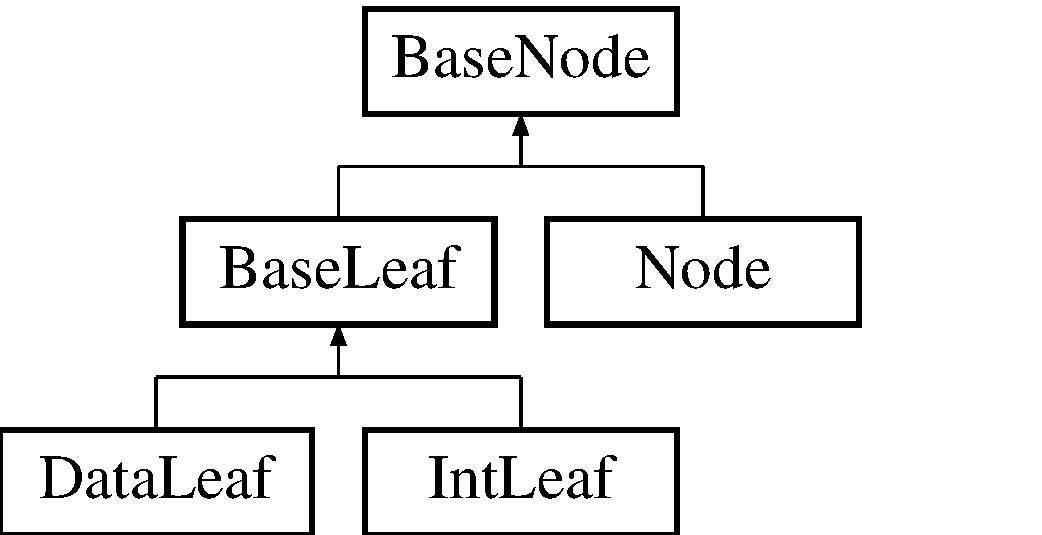
\includegraphics[height=3.000000cm]{class_base_node}
\end{center}
\end{figure}
\subsection*{Public Types}
\begin{DoxyCompactItemize}
\item 
enum \hyperlink{class_base_node_a01f9336072c3fb197a2a0dda45d78544}{Node\-Type} \{ \hyperlink{class_base_node_a01f9336072c3fb197a2a0dda45d78544a528465af535d31fc21605e0c41ac4bc1}{N\-O\-D\-E} = 0, 
\hyperlink{class_base_node_a01f9336072c3fb197a2a0dda45d78544a19c8347aacceaf071d7a9ebada297de3}{I\-N\-T\-\_\-\-L\-E\-A\-F} = 1, 
\hyperlink{class_base_node_a01f9336072c3fb197a2a0dda45d78544a3a9022b38c3db828c6479d21994962c4}{D\-A\-T\-A\-\_\-\-L\-E\-A\-F} = 2
 \}
\end{DoxyCompactItemize}
\subsection*{Public Member Functions}
\begin{DoxyCompactItemize}
\item 
\hyperlink{class_base_node_afc5bd25898054b2e50d6b01451d73b1b}{Base\-Node} (\hyperlink{class_base_node_a01f9336072c3fb197a2a0dda45d78544}{Base\-Node\-::\-Node\-Type} type)
\item 
\hyperlink{class_base_node_a27d5e3b508b19fa7887ac95d15a46f9c}{$\sim$\-Base\-Node} (void)
\item 
\hyperlink{class_base_node_a01f9336072c3fb197a2a0dda45d78544}{Base\-Node\-::\-Node\-Type} \hyperlink{class_base_node_a080bb4228cc6b0239f29c033257c486e}{get\-Type} (void) const 
\item 
virtual int32\-\_\-t \hyperlink{class_base_node_a50aef77f988f7689e96b346705628f91}{get\-Length} (void) const =0
\item 
virtual \hyperlink{types_8h_a64b5be62be31dcda165d2c6c3c262fb5}{bytevector} \hyperlink{class_base_node_aad2eb87014be9a786ec9a4c4ac405c45}{to\-Vector} (void) const =0
\item 
\hyperlink{types_8h_a64b5be62be31dcda165d2c6c3c262fb5}{bytevector} \hyperlink{class_base_node_aa5206e6e347794cba4068ddd90b8a091}{serialize} () const 
\item 
\hyperlink{types_8h_a64b5be62be31dcda165d2c6c3c262fb5}{bytevector} \hyperlink{class_base_node_ab9ec930839c38803c8be0638c7096982}{concat\-Data} (const \hyperlink{class_base_node}{Base\-Node} $\ast$const other) const 
\end{DoxyCompactItemize}
\subsection*{Static Protected Member Functions}
\begin{DoxyCompactItemize}
\item 
static \hyperlink{class_base_node}{Base\-Node} $\ast$ \hyperlink{class_base_node_ae7b4733f4f9eae9979dc9d8469d51c28}{copy} (const \hyperlink{class_base_node}{Base\-Node} $\ast$node)
\item 
static void \hyperlink{class_base_node_ae2e188a31e6eb5d04caa4e57314a7f51}{Read\-Node\-Header} (std\-::istream \&file, char \&type, uint32\-\_\-t \&length)
\end{DoxyCompactItemize}


\subsection{Detailed Description}
The basic node from which all nodes in a Byte Tree inherit. 

\subsection{Member Enumeration Documentation}
\hypertarget{class_base_node_a01f9336072c3fb197a2a0dda45d78544}{\index{Base\-Node@{Base\-Node}!Node\-Type@{Node\-Type}}
\index{Node\-Type@{Node\-Type}!BaseNode@{Base\-Node}}
\subsubsection[{Node\-Type}]{\setlength{\rightskip}{0pt plus 5cm}enum {\bf Base\-Node\-::\-Node\-Type}}}\label{class_base_node_a01f9336072c3fb197a2a0dda45d78544}
\begin{Desc}
\item[Enumerator]\par
\begin{description}
\index{N\-O\-D\-E@{N\-O\-D\-E}!Base\-Node@{Base\-Node}}\index{Base\-Node@{Base\-Node}!N\-O\-D\-E@{N\-O\-D\-E}}\item[{\em 
\hypertarget{class_base_node_a01f9336072c3fb197a2a0dda45d78544a528465af535d31fc21605e0c41ac4bc1}{N\-O\-D\-E}\label{class_base_node_a01f9336072c3fb197a2a0dda45d78544a528465af535d31fc21605e0c41ac4bc1}
}]A node which contains other nodes. \index{I\-N\-T\-\_\-\-L\-E\-A\-F@{I\-N\-T\-\_\-\-L\-E\-A\-F}!Base\-Node@{Base\-Node}}\index{Base\-Node@{Base\-Node}!I\-N\-T\-\_\-\-L\-E\-A\-F@{I\-N\-T\-\_\-\-L\-E\-A\-F}}\item[{\em 
\hypertarget{class_base_node_a01f9336072c3fb197a2a0dda45d78544a19c8347aacceaf071d7a9ebada297de3}{I\-N\-T\-\_\-\-L\-E\-A\-F}\label{class_base_node_a01f9336072c3fb197a2a0dda45d78544a19c8347aacceaf071d7a9ebada297de3}
}]An \hyperlink{class_int_leaf}{Int\-Leaf} which contains a number. \index{D\-A\-T\-A\-\_\-\-L\-E\-A\-F@{D\-A\-T\-A\-\_\-\-L\-E\-A\-F}!Base\-Node@{Base\-Node}}\index{Base\-Node@{Base\-Node}!D\-A\-T\-A\-\_\-\-L\-E\-A\-F@{D\-A\-T\-A\-\_\-\-L\-E\-A\-F}}\item[{\em 
\hypertarget{class_base_node_a01f9336072c3fb197a2a0dda45d78544a3a9022b38c3db828c6479d21994962c4}{D\-A\-T\-A\-\_\-\-L\-E\-A\-F}\label{class_base_node_a01f9336072c3fb197a2a0dda45d78544a3a9022b38c3db828c6479d21994962c4}
}]A \hyperlink{class_data_leaf}{Data\-Leaf} which contains a string or vector of bytes. \end{description}
\end{Desc}


\subsection{Constructor \& Destructor Documentation}
\hypertarget{class_base_node_afc5bd25898054b2e50d6b01451d73b1b}{\index{Base\-Node@{Base\-Node}!Base\-Node@{Base\-Node}}
\index{Base\-Node@{Base\-Node}!BaseNode@{Base\-Node}}
\subsubsection[{Base\-Node}]{\setlength{\rightskip}{0pt plus 5cm}Base\-Node\-::\-Base\-Node (
\begin{DoxyParamCaption}
\item[{{\bf Base\-Node\-::\-Node\-Type}}]{type}
\end{DoxyParamCaption}
)}}\label{class_base_node_afc5bd25898054b2e50d6b01451d73b1b}
\hypertarget{class_base_node_a27d5e3b508b19fa7887ac95d15a46f9c}{\index{Base\-Node@{Base\-Node}!$\sim$\-Base\-Node@{$\sim$\-Base\-Node}}
\index{$\sim$\-Base\-Node@{$\sim$\-Base\-Node}!BaseNode@{Base\-Node}}
\subsubsection[{$\sim$\-Base\-Node}]{\setlength{\rightskip}{0pt plus 5cm}Base\-Node\-::$\sim$\-Base\-Node (
\begin{DoxyParamCaption}
\item[{void}]{}
\end{DoxyParamCaption}
)}}\label{class_base_node_a27d5e3b508b19fa7887ac95d15a46f9c}


\subsection{Member Function Documentation}
\hypertarget{class_base_node_ab9ec930839c38803c8be0638c7096982}{\index{Base\-Node@{Base\-Node}!concat\-Data@{concat\-Data}}
\index{concat\-Data@{concat\-Data}!BaseNode@{Base\-Node}}
\subsubsection[{concat\-Data}]{\setlength{\rightskip}{0pt plus 5cm}{\bf bytevector} Base\-Node\-::concat\-Data (
\begin{DoxyParamCaption}
\item[{const {\bf Base\-Node} $\ast$const}]{other}
\end{DoxyParamCaption}
) const}}\label{class_base_node_ab9ec930839c38803c8be0638c7096982}
\hypertarget{class_base_node_ae7b4733f4f9eae9979dc9d8469d51c28}{\index{Base\-Node@{Base\-Node}!copy@{copy}}
\index{copy@{copy}!BaseNode@{Base\-Node}}
\subsubsection[{copy}]{\setlength{\rightskip}{0pt plus 5cm}{\bf Base\-Node} $\ast$ Base\-Node\-::copy (
\begin{DoxyParamCaption}
\item[{const {\bf Base\-Node} $\ast$}]{node}
\end{DoxyParamCaption}
)\hspace{0.3cm}{\ttfamily [static]}, {\ttfamily [protected]}}}\label{class_base_node_ae7b4733f4f9eae9979dc9d8469d51c28}
\hypertarget{class_base_node_a50aef77f988f7689e96b346705628f91}{\index{Base\-Node@{Base\-Node}!get\-Length@{get\-Length}}
\index{get\-Length@{get\-Length}!BaseNode@{Base\-Node}}
\subsubsection[{get\-Length}]{\setlength{\rightskip}{0pt plus 5cm}virtual int32\-\_\-t Base\-Node\-::get\-Length (
\begin{DoxyParamCaption}
\item[{void}]{}
\end{DoxyParamCaption}
) const\hspace{0.3cm}{\ttfamily [pure virtual]}}}\label{class_base_node_a50aef77f988f7689e96b346705628f91}


Implemented in \hyperlink{class_node_ad602104b3c245a564f741b65fe97845c}{Node}, \hyperlink{class_int_leaf_a92719f80a7410d76e4fae51de9b28e36}{Int\-Leaf}, and \hyperlink{class_data_leaf_aba4c714ea1dc591023298c50a2e18523}{Data\-Leaf}.

\hypertarget{class_base_node_a080bb4228cc6b0239f29c033257c486e}{\index{Base\-Node@{Base\-Node}!get\-Type@{get\-Type}}
\index{get\-Type@{get\-Type}!BaseNode@{Base\-Node}}
\subsubsection[{get\-Type}]{\setlength{\rightskip}{0pt plus 5cm}{\bf Base\-Node\-::\-Node\-Type} Base\-Node\-::get\-Type (
\begin{DoxyParamCaption}
\item[{void}]{}
\end{DoxyParamCaption}
) const}}\label{class_base_node_a080bb4228cc6b0239f29c033257c486e}
\hypertarget{class_base_node_ae2e188a31e6eb5d04caa4e57314a7f51}{\index{Base\-Node@{Base\-Node}!Read\-Node\-Header@{Read\-Node\-Header}}
\index{Read\-Node\-Header@{Read\-Node\-Header}!BaseNode@{Base\-Node}}
\subsubsection[{Read\-Node\-Header}]{\setlength{\rightskip}{0pt plus 5cm}void Base\-Node\-::\-Read\-Node\-Header (
\begin{DoxyParamCaption}
\item[{std\-::istream \&}]{file, }
\item[{char \&}]{type, }
\item[{uint32\-\_\-t \&}]{length}
\end{DoxyParamCaption}
)\hspace{0.3cm}{\ttfamily [static]}, {\ttfamily [protected]}}}\label{class_base_node_ae2e188a31e6eb5d04caa4e57314a7f51}
\hypertarget{class_base_node_aa5206e6e347794cba4068ddd90b8a091}{\index{Base\-Node@{Base\-Node}!serialize@{serialize}}
\index{serialize@{serialize}!BaseNode@{Base\-Node}}
\subsubsection[{serialize}]{\setlength{\rightskip}{0pt plus 5cm}{\bf bytevector} Base\-Node\-::serialize (
\begin{DoxyParamCaption}
{}
\end{DoxyParamCaption}
) const}}\label{class_base_node_aa5206e6e347794cba4068ddd90b8a091}
\hypertarget{class_base_node_aad2eb87014be9a786ec9a4c4ac405c45}{\index{Base\-Node@{Base\-Node}!to\-Vector@{to\-Vector}}
\index{to\-Vector@{to\-Vector}!BaseNode@{Base\-Node}}
\subsubsection[{to\-Vector}]{\setlength{\rightskip}{0pt plus 5cm}virtual {\bf bytevector} Base\-Node\-::to\-Vector (
\begin{DoxyParamCaption}
\item[{void}]{}
\end{DoxyParamCaption}
) const\hspace{0.3cm}{\ttfamily [pure virtual]}}}\label{class_base_node_aad2eb87014be9a786ec9a4c4ac405c45}


Implemented in \hyperlink{class_int_leaf_a1817ac7916ab1c4ff09717db0a6d95f2}{Int\-Leaf}, \hyperlink{class_node_a858d4b4757880eba1fdead1412418693}{Node}, and \hyperlink{class_data_leaf_a62ce63296d298d6ffdc133dafe3b281f}{Data\-Leaf}.



The documentation for this class was generated from the following files\-:\begin{DoxyCompactItemize}
\item 
Arithmetic/\hyperlink{_base_node_8h}{Base\-Node.\-h}\item 
Arithmetic/\hyperlink{_base_node_8cpp}{Base\-Node.\-cpp}\end{DoxyCompactItemize}

\hypertarget{class_data_leaf}{\section{Data\-Leaf Class Reference}
\label{class_data_leaf}\index{Data\-Leaf@{Data\-Leaf}}
}


{\ttfamily \#include $<$Data\-Leaf.\-h$>$}

Inheritance diagram for Data\-Leaf\-:\begin{figure}[H]
\begin{center}
\leavevmode
\includegraphics[height=3.000000cm]{class_data_leaf}
\end{center}
\end{figure}
\subsection*{Public Member Functions}
\begin{DoxyCompactItemize}
\item 
\hyperlink{class_data_leaf_ac9a64badc57c7e8a72b2e437986026a9}{Data\-Leaf} (void)
\item 
\hyperlink{class_data_leaf_a41c683e5c39dd83f26f200ca310d2921}{Data\-Leaf} (int32\-\_\-t size)
\item 
\hyperlink{class_data_leaf_a047de3114cfe3918d11e367ba6d37b2b}{Data\-Leaf} (std\-::istream \&file)
\item 
\hyperlink{class_data_leaf_a40b50e7b1c36769a64ed1166dcaaf1a6}{Data\-Leaf} (std\-::string str)
\item 
\hyperlink{class_data_leaf_a09bb67c6dd0d8841b03b63332416a479}{$\sim$\-Data\-Leaf} (void)
\item 
\hyperlink{types_8h_a64b5be62be31dcda165d2c6c3c262fb5}{bytevector} \& \hyperlink{class_data_leaf_aee63c9d1396d62386e7f22dcbdc1386c}{get\-Data} (void)
\item 
const \hyperlink{types_8h_a64b5be62be31dcda165d2c6c3c262fb5}{bytevector} \& \hyperlink{class_data_leaf_a49a48425860d4ef538b3b9c6ea755a35}{get\-Data} (void) const 
\item 
virtual \hyperlink{types_8h_a64b5be62be31dcda165d2c6c3c262fb5}{bytevector} \hyperlink{class_data_leaf_a62ce63296d298d6ffdc133dafe3b281f}{to\-Vector} (void) const 
\item 
virtual int32\-\_\-t \hyperlink{class_data_leaf_aba4c714ea1dc591023298c50a2e18523}{get\-Length} (void) const 
\item 
\hyperlink{class_data_leaf}{Data\-Leaf} \& \hyperlink{class_data_leaf_a6ea1eda11735b909ae61972a7af919c5}{operator=} (const \hyperlink{class_data_leaf}{Data\-Leaf} \&leaf)
\end{DoxyCompactItemize}
\subsection*{Additional Inherited Members}


\subsection{Constructor \& Destructor Documentation}
\hypertarget{class_data_leaf_ac9a64badc57c7e8a72b2e437986026a9}{\index{Data\-Leaf@{Data\-Leaf}!Data\-Leaf@{Data\-Leaf}}
\index{Data\-Leaf@{Data\-Leaf}!DataLeaf@{Data\-Leaf}}
\subsubsection[{Data\-Leaf}]{\setlength{\rightskip}{0pt plus 5cm}Data\-Leaf\-::\-Data\-Leaf (
\begin{DoxyParamCaption}
\item[{void}]{}
\end{DoxyParamCaption}
)}}\label{class_data_leaf_ac9a64badc57c7e8a72b2e437986026a9}
\hypertarget{class_data_leaf_a41c683e5c39dd83f26f200ca310d2921}{\index{Data\-Leaf@{Data\-Leaf}!Data\-Leaf@{Data\-Leaf}}
\index{Data\-Leaf@{Data\-Leaf}!DataLeaf@{Data\-Leaf}}
\subsubsection[{Data\-Leaf}]{\setlength{\rightskip}{0pt plus 5cm}Data\-Leaf\-::\-Data\-Leaf (
\begin{DoxyParamCaption}
\item[{int32\-\_\-t}]{size}
\end{DoxyParamCaption}
)\hspace{0.3cm}{\ttfamily [explicit]}}}\label{class_data_leaf_a41c683e5c39dd83f26f200ca310d2921}
\hypertarget{class_data_leaf_a047de3114cfe3918d11e367ba6d37b2b}{\index{Data\-Leaf@{Data\-Leaf}!Data\-Leaf@{Data\-Leaf}}
\index{Data\-Leaf@{Data\-Leaf}!DataLeaf@{Data\-Leaf}}
\subsubsection[{Data\-Leaf}]{\setlength{\rightskip}{0pt plus 5cm}Data\-Leaf\-::\-Data\-Leaf (
\begin{DoxyParamCaption}
\item[{std\-::istream \&}]{file}
\end{DoxyParamCaption}
)}}\label{class_data_leaf_a047de3114cfe3918d11e367ba6d37b2b}
\hypertarget{class_data_leaf_a40b50e7b1c36769a64ed1166dcaaf1a6}{\index{Data\-Leaf@{Data\-Leaf}!Data\-Leaf@{Data\-Leaf}}
\index{Data\-Leaf@{Data\-Leaf}!DataLeaf@{Data\-Leaf}}
\subsubsection[{Data\-Leaf}]{\setlength{\rightskip}{0pt plus 5cm}Data\-Leaf\-::\-Data\-Leaf (
\begin{DoxyParamCaption}
\item[{std\-::string}]{str}
\end{DoxyParamCaption}
)}}\label{class_data_leaf_a40b50e7b1c36769a64ed1166dcaaf1a6}
\hypertarget{class_data_leaf_a09bb67c6dd0d8841b03b63332416a479}{\index{Data\-Leaf@{Data\-Leaf}!$\sim$\-Data\-Leaf@{$\sim$\-Data\-Leaf}}
\index{$\sim$\-Data\-Leaf@{$\sim$\-Data\-Leaf}!DataLeaf@{Data\-Leaf}}
\subsubsection[{$\sim$\-Data\-Leaf}]{\setlength{\rightskip}{0pt plus 5cm}Data\-Leaf\-::$\sim$\-Data\-Leaf (
\begin{DoxyParamCaption}
\item[{void}]{}
\end{DoxyParamCaption}
)}}\label{class_data_leaf_a09bb67c6dd0d8841b03b63332416a479}


\subsection{Member Function Documentation}
\hypertarget{class_data_leaf_aee63c9d1396d62386e7f22dcbdc1386c}{\index{Data\-Leaf@{Data\-Leaf}!get\-Data@{get\-Data}}
\index{get\-Data@{get\-Data}!DataLeaf@{Data\-Leaf}}
\subsubsection[{get\-Data}]{\setlength{\rightskip}{0pt plus 5cm}{\bf bytevector} \& Data\-Leaf\-::get\-Data (
\begin{DoxyParamCaption}
\item[{void}]{}
\end{DoxyParamCaption}
)}}\label{class_data_leaf_aee63c9d1396d62386e7f22dcbdc1386c}
\hypertarget{class_data_leaf_a49a48425860d4ef538b3b9c6ea755a35}{\index{Data\-Leaf@{Data\-Leaf}!get\-Data@{get\-Data}}
\index{get\-Data@{get\-Data}!DataLeaf@{Data\-Leaf}}
\subsubsection[{get\-Data}]{\setlength{\rightskip}{0pt plus 5cm}const {\bf bytevector} \& Data\-Leaf\-::get\-Data (
\begin{DoxyParamCaption}
\item[{void}]{}
\end{DoxyParamCaption}
) const}}\label{class_data_leaf_a49a48425860d4ef538b3b9c6ea755a35}
\hypertarget{class_data_leaf_aba4c714ea1dc591023298c50a2e18523}{\index{Data\-Leaf@{Data\-Leaf}!get\-Length@{get\-Length}}
\index{get\-Length@{get\-Length}!DataLeaf@{Data\-Leaf}}
\subsubsection[{get\-Length}]{\setlength{\rightskip}{0pt plus 5cm}int32\-\_\-t Data\-Leaf\-::get\-Length (
\begin{DoxyParamCaption}
\item[{void}]{}
\end{DoxyParamCaption}
) const\hspace{0.3cm}{\ttfamily [virtual]}}}\label{class_data_leaf_aba4c714ea1dc591023298c50a2e18523}


Implements \hyperlink{class_base_node_a50aef77f988f7689e96b346705628f91}{Base\-Node}.

\hypertarget{class_data_leaf_a6ea1eda11735b909ae61972a7af919c5}{\index{Data\-Leaf@{Data\-Leaf}!operator=@{operator=}}
\index{operator=@{operator=}!DataLeaf@{Data\-Leaf}}
\subsubsection[{operator=}]{\setlength{\rightskip}{0pt plus 5cm}{\bf Data\-Leaf} \& Data\-Leaf\-::operator= (
\begin{DoxyParamCaption}
\item[{const {\bf Data\-Leaf} \&}]{leaf}
\end{DoxyParamCaption}
)}}\label{class_data_leaf_a6ea1eda11735b909ae61972a7af919c5}
\hypertarget{class_data_leaf_a62ce63296d298d6ffdc133dafe3b281f}{\index{Data\-Leaf@{Data\-Leaf}!to\-Vector@{to\-Vector}}
\index{to\-Vector@{to\-Vector}!DataLeaf@{Data\-Leaf}}
\subsubsection[{to\-Vector}]{\setlength{\rightskip}{0pt plus 5cm}{\bf bytevector} Data\-Leaf\-::to\-Vector (
\begin{DoxyParamCaption}
\item[{void}]{}
\end{DoxyParamCaption}
) const\hspace{0.3cm}{\ttfamily [virtual]}}}\label{class_data_leaf_a62ce63296d298d6ffdc133dafe3b281f}


Implements \hyperlink{class_base_node_aad2eb87014be9a786ec9a4c4ac405c45}{Base\-Node}.



The documentation for this class was generated from the following files\-:\begin{DoxyCompactItemize}
\item 
Arithmetic/\hyperlink{_data_leaf_8h}{Data\-Leaf.\-h}\item 
Arithmetic/\hyperlink{_data_leaf_8cpp}{Data\-Leaf.\-cpp}\end{DoxyCompactItemize}

\hypertarget{class_int_leaf}{\section{Int\-Leaf Class Reference}
\label{class_int_leaf}\index{Int\-Leaf@{Int\-Leaf}}
}


{\ttfamily \#include $<$Int\-Leaf.\-h$>$}

Inheritance diagram for Int\-Leaf\-:\begin{figure}[H]
\begin{center}
\leavevmode
\includegraphics[height=3.000000cm]{class_int_leaf}
\end{center}
\end{figure}
\subsection*{Public Member Functions}
\begin{DoxyCompactItemize}
\item 
\hyperlink{class_int_leaf_a1edff3e6ab3ccf64907420ac84d71b70}{Int\-Leaf} (void)
\item 
\hyperlink{class_int_leaf_a06aaabf11bc0d0851e3df7b705ca1ccb}{Int\-Leaf} (const \hyperlink{class_int_leaf}{Int\-Leaf} \&leaf)
\item 
\hyperlink{class_int_leaf_affd60a076c8a9f1be25644a8d17a939b}{Int\-Leaf} (const mpz\-\_\-class \&bigint)
\item 
\hyperlink{class_int_leaf_a65e0a79456dc0b8fd1d33c03991b3848}{Int\-Leaf} (long int input)
\item 
\hyperlink{class_int_leaf_adfcd1af6b8cd149609c00170cb3380e6}{Int\-Leaf} (long int input, long int length)
\item 
\hyperlink{class_int_leaf_a7fae91565854dcf68de2a6730f56cce3}{Int\-Leaf} (std\-::string input)
\item 
\hyperlink{class_int_leaf_ad115e1df24da76baedaacc1543ae33cd}{Int\-Leaf} (\hyperlink{types_8h_a64b5be62be31dcda165d2c6c3c262fb5}{bytevector} bytevec)
\item 
\hyperlink{class_int_leaf_a59d3493348dc590c5b2021d63049ec1e}{Int\-Leaf} (std\-::istream \&file)
\item 
\hyperlink{class_int_leaf_a098a7534215db34214dd1302cc963758}{$\sim$\-Int\-Leaf} (void)
\item 
\hyperlink{class_int_leaf}{Int\-Leaf} \& \hyperlink{class_int_leaf_a9bbc6aea2aecae8c20288c6917b3523e}{operator=} (const \hyperlink{class_int_leaf}{Int\-Leaf} \&leaf)
\item 
\hyperlink{class_int_leaf}{Int\-Leaf} \& \hyperlink{class_int_leaf_a80707cbdf1e4fdfd705acb6b1e0b445c}{operator=} (long int input)
\item 
\hyperlink{class_int_leaf}{Int\-Leaf} \& \hyperlink{class_int_leaf_a4447ab3008de3bb7cda20715e72b11a0}{operator=} (std\-::string input)
\item 
\hyperlink{class_int_leaf}{Int\-Leaf} \& \hyperlink{class_int_leaf_a691407858bdc596bc1be48f8d3ae9c62}{mod\-To} (const \hyperlink{class_int_leaf}{Int\-Leaf} \&leaf)
\item 
\hyperlink{class_int_leaf}{Int\-Leaf} \hyperlink{class_int_leaf_a4e645145141d0f8ded8afdd2c6aa7228}{mod} (const \hyperlink{class_int_leaf}{Int\-Leaf} \&leaf) const 
\item 
\hyperlink{class_int_leaf}{Int\-Leaf} \& \hyperlink{class_int_leaf_aa01577692f0e8ae228ecd269f81d7f1c}{add\-To} (const \hyperlink{class_int_leaf}{Int\-Leaf} \&leaf)
\item 
\hyperlink{class_int_leaf}{Int\-Leaf} \hyperlink{class_int_leaf_abb3c9fbe230ea366d6bc535c0bdec914}{add} (const \hyperlink{class_int_leaf}{Int\-Leaf} \&leaf) const 
\item 
\hyperlink{class_int_leaf}{Int\-Leaf} \& \hyperlink{class_int_leaf_ac41a9c6bd62f3e1bb8e9befcaf6d4675}{add\-To\-Mod} (const \hyperlink{class_int_leaf}{Int\-Leaf} \&leaf, const \hyperlink{class_int_leaf}{Int\-Leaf} \&\hyperlink{class_int_leaf_a4e645145141d0f8ded8afdd2c6aa7228}{mod})
\item 
\hyperlink{class_int_leaf}{Int\-Leaf} \hyperlink{class_int_leaf_a18fdf94a11a9cc1c27d5fd35449a1ae3}{add\-Mod} (const \hyperlink{class_int_leaf}{Int\-Leaf} \&leaf, const \hyperlink{class_int_leaf}{Int\-Leaf} \&\hyperlink{class_int_leaf_a4e645145141d0f8ded8afdd2c6aa7228}{mod}) const 
\item 
\hyperlink{class_int_leaf}{Int\-Leaf} \& \hyperlink{class_int_leaf_ac3832b8f8dbabb25c182cffd7a1cf848}{operator+=} (const \hyperlink{class_int_leaf}{Int\-Leaf} \&leaf)
\item 
\hyperlink{class_int_leaf}{Int\-Leaf} \hyperlink{class_int_leaf_abac0513d6fad2231b96f8af527d5762e}{operator+} (const \hyperlink{class_int_leaf}{Int\-Leaf} \&leaf) const 
\item 
\hyperlink{class_int_leaf}{Int\-Leaf} \& \hyperlink{class_int_leaf_a977132f0c126e46eaad34ed93c683727}{mult\-To} (const \hyperlink{class_int_leaf}{Int\-Leaf} \&leaf)
\item 
\hyperlink{class_int_leaf}{Int\-Leaf} \hyperlink{class_int_leaf_ad4635cd5bc4fddb9e4db5ebfc523e33f}{mult} (const \hyperlink{class_int_leaf}{Int\-Leaf} \&leaf) const 
\item 
\hyperlink{class_int_leaf}{Int\-Leaf} \& \hyperlink{class_int_leaf_a5f893aa4d1954a0c273f02413a662ca5}{mult\-To\-Mod} (const \hyperlink{class_int_leaf}{Int\-Leaf} \&leaf, const \hyperlink{class_int_leaf}{Int\-Leaf} \&\hyperlink{class_int_leaf_a4e645145141d0f8ded8afdd2c6aa7228}{mod})
\item 
\hyperlink{class_int_leaf}{Int\-Leaf} \hyperlink{class_int_leaf_a1d24e8b786d5736c637a24ea5d90ef0d}{mult\-Mod} (const \hyperlink{class_int_leaf}{Int\-Leaf} \&leaf, const \hyperlink{class_int_leaf}{Int\-Leaf} \&\hyperlink{class_int_leaf_a4e645145141d0f8ded8afdd2c6aa7228}{mod}) const 
\item 
\hyperlink{class_int_leaf}{Int\-Leaf} \& \hyperlink{class_int_leaf_a223e80a00ae1d5b6406202390c530350}{operator$\ast$=} (const \hyperlink{class_int_leaf}{Int\-Leaf} \&leaf)
\item 
\hyperlink{class_int_leaf}{Int\-Leaf} \hyperlink{class_int_leaf_a4c61097359b76a570a2694540fe50353}{operator$\ast$} (const \hyperlink{class_int_leaf}{Int\-Leaf} \&leaf) const 
\item 
\hyperlink{class_int_leaf}{Int\-Leaf} \& \hyperlink{class_int_leaf_a4f3e611a11145013b51d60858ef92d27}{exp\-To} (unsigned long exponent)
\item 
\hyperlink{class_int_leaf}{Int\-Leaf} \hyperlink{class_int_leaf_ad0c837ec28fe24e02e61f252b5f984ea}{exp} (unsigned long exponent) const 
\item 
\hyperlink{class_int_leaf}{Int\-Leaf} \& \hyperlink{class_int_leaf_a27195b157fbfc3610c805319d45ebbed}{exp\-To\-Mod} (const \hyperlink{class_int_leaf}{Int\-Leaf} \&leaf, const \hyperlink{class_int_leaf}{Int\-Leaf} \&\hyperlink{class_int_leaf_a4e645145141d0f8ded8afdd2c6aa7228}{mod})
\item 
\hyperlink{class_int_leaf}{Int\-Leaf} \hyperlink{class_int_leaf_ab9be4f972ddaa79d5482b2f037476ea8}{exp\-Mod} (const \hyperlink{class_int_leaf}{Int\-Leaf} \&leaf, const \hyperlink{class_int_leaf}{Int\-Leaf} \&\hyperlink{class_int_leaf_a4e645145141d0f8ded8afdd2c6aa7228}{mod}) const 
\item 
bool \hyperlink{class_int_leaf_a315436fad53849eb1701b665c12d3682}{operator==} (const \hyperlink{class_int_leaf}{Int\-Leaf} \&leaf) const 
\item 
bool \hyperlink{class_int_leaf_adf2a7f85887432129ae1a6fd200ebcbb}{operator!=} (const \hyperlink{class_int_leaf}{Int\-Leaf} \&leaf) const 
\item 
bool \hyperlink{class_int_leaf_ae62d5927bd7b6b91961b8cd0f9a25873}{operator$<$} (const \hyperlink{class_int_leaf}{Int\-Leaf} \&leaf) const 
\item 
bool \hyperlink{class_int_leaf_a1ad7269c9e92c87612f81bb665a973f9}{operator$>$} (const \hyperlink{class_int_leaf}{Int\-Leaf} \&leaf) const 
\item 
\hyperlink{class_int_leaf}{Int\-Leaf} \hyperlink{class_int_leaf_ad12dc34eca055a28ecfb6ea469d4e887}{operator-\/} (void) const 
\item 
\hyperlink{class_int_leaf}{Int\-Leaf} \hyperlink{class_int_leaf_ab27881e338fb850a3cb59fd3e502339e}{inverse} (const \hyperlink{class_int_leaf}{Int\-Leaf} \&\hyperlink{class_int_leaf_a4e645145141d0f8ded8afdd2c6aa7228}{mod}) const 
\item 
mpz\-\_\-class \hyperlink{class_int_leaf_a519d2f9d31a01c3e90d898156631b7a2}{get\-Big\-Int} (void) const 
\item 
virtual \hyperlink{types_8h_a64b5be62be31dcda165d2c6c3c262fb5}{bytevector} \hyperlink{class_int_leaf_a1817ac7916ab1c4ff09717db0a6d95f2}{to\-Vector} (void) const 
\item 
virtual int32\-\_\-t \hyperlink{class_int_leaf_a92719f80a7410d76e4fae51de9b28e36}{get\-Length} (void) const 
\item 
std\-::string \hyperlink{class_int_leaf_ad816e278b0955fd58bbbb1669b8d6885}{to\-String} (void) const 
\end{DoxyCompactItemize}
\subsection*{Static Public Member Functions}
\begin{DoxyCompactItemize}
\item 
static \hyperlink{class_base_node}{Base\-Node} $\ast$ \hyperlink{class_int_leaf_aeedcffeab76e98891ed98a235696c3db}{construct\-Part\-From\-File} (std\-::istream \&file, uint32\-\_\-t length)
\end{DoxyCompactItemize}
\subsection*{Static Public Attributes}
\begin{DoxyCompactItemize}
\item 
static const int \hyperlink{class_int_leaf_af01a2d863b6f746f3f0b2ca7fa283561}{A\-R\-R\-A\-Y\-O\-R\-D\-E\-R} = 1
\item 
static const int \hyperlink{class_int_leaf_a3114b538c3c64d8013ab7823377703ce}{E\-N\-D\-I\-A\-N} = 0
\item 
static const int \hyperlink{class_int_leaf_a4827cc727b294e977a03881ff3b852d6}{N\-A\-I\-L\-S} = 0
\end{DoxyCompactItemize}
\subsection*{Additional Inherited Members}


\subsection{Constructor \& Destructor Documentation}
\hypertarget{class_int_leaf_a1edff3e6ab3ccf64907420ac84d71b70}{\index{Int\-Leaf@{Int\-Leaf}!Int\-Leaf@{Int\-Leaf}}
\index{Int\-Leaf@{Int\-Leaf}!IntLeaf@{Int\-Leaf}}
\subsubsection[{Int\-Leaf}]{\setlength{\rightskip}{0pt plus 5cm}Int\-Leaf\-::\-Int\-Leaf (
\begin{DoxyParamCaption}
\item[{void}]{}
\end{DoxyParamCaption}
)}}\label{class_int_leaf_a1edff3e6ab3ccf64907420ac84d71b70}
\hypertarget{class_int_leaf_a06aaabf11bc0d0851e3df7b705ca1ccb}{\index{Int\-Leaf@{Int\-Leaf}!Int\-Leaf@{Int\-Leaf}}
\index{Int\-Leaf@{Int\-Leaf}!IntLeaf@{Int\-Leaf}}
\subsubsection[{Int\-Leaf}]{\setlength{\rightskip}{0pt plus 5cm}Int\-Leaf\-::\-Int\-Leaf (
\begin{DoxyParamCaption}
\item[{const {\bf Int\-Leaf} \&}]{leaf}
\end{DoxyParamCaption}
)}}\label{class_int_leaf_a06aaabf11bc0d0851e3df7b705ca1ccb}
\hypertarget{class_int_leaf_affd60a076c8a9f1be25644a8d17a939b}{\index{Int\-Leaf@{Int\-Leaf}!Int\-Leaf@{Int\-Leaf}}
\index{Int\-Leaf@{Int\-Leaf}!IntLeaf@{Int\-Leaf}}
\subsubsection[{Int\-Leaf}]{\setlength{\rightskip}{0pt plus 5cm}Int\-Leaf\-::\-Int\-Leaf (
\begin{DoxyParamCaption}
\item[{const mpz\-\_\-class \&}]{bigint}
\end{DoxyParamCaption}
)\hspace{0.3cm}{\ttfamily [explicit]}}}\label{class_int_leaf_affd60a076c8a9f1be25644a8d17a939b}
\hypertarget{class_int_leaf_a65e0a79456dc0b8fd1d33c03991b3848}{\index{Int\-Leaf@{Int\-Leaf}!Int\-Leaf@{Int\-Leaf}}
\index{Int\-Leaf@{Int\-Leaf}!IntLeaf@{Int\-Leaf}}
\subsubsection[{Int\-Leaf}]{\setlength{\rightskip}{0pt plus 5cm}Int\-Leaf\-::\-Int\-Leaf (
\begin{DoxyParamCaption}
\item[{long int}]{input}
\end{DoxyParamCaption}
)}}\label{class_int_leaf_a65e0a79456dc0b8fd1d33c03991b3848}
\hypertarget{class_int_leaf_adfcd1af6b8cd149609c00170cb3380e6}{\index{Int\-Leaf@{Int\-Leaf}!Int\-Leaf@{Int\-Leaf}}
\index{Int\-Leaf@{Int\-Leaf}!IntLeaf@{Int\-Leaf}}
\subsubsection[{Int\-Leaf}]{\setlength{\rightskip}{0pt plus 5cm}Int\-Leaf\-::\-Int\-Leaf (
\begin{DoxyParamCaption}
\item[{long int}]{input, }
\item[{long int}]{length}
\end{DoxyParamCaption}
)}}\label{class_int_leaf_adfcd1af6b8cd149609c00170cb3380e6}
\hypertarget{class_int_leaf_a7fae91565854dcf68de2a6730f56cce3}{\index{Int\-Leaf@{Int\-Leaf}!Int\-Leaf@{Int\-Leaf}}
\index{Int\-Leaf@{Int\-Leaf}!IntLeaf@{Int\-Leaf}}
\subsubsection[{Int\-Leaf}]{\setlength{\rightskip}{0pt plus 5cm}Int\-Leaf\-::\-Int\-Leaf (
\begin{DoxyParamCaption}
\item[{std\-::string}]{input}
\end{DoxyParamCaption}
)\hspace{0.3cm}{\ttfamily [explicit]}}}\label{class_int_leaf_a7fae91565854dcf68de2a6730f56cce3}
\hypertarget{class_int_leaf_ad115e1df24da76baedaacc1543ae33cd}{\index{Int\-Leaf@{Int\-Leaf}!Int\-Leaf@{Int\-Leaf}}
\index{Int\-Leaf@{Int\-Leaf}!IntLeaf@{Int\-Leaf}}
\subsubsection[{Int\-Leaf}]{\setlength{\rightskip}{0pt plus 5cm}Int\-Leaf\-::\-Int\-Leaf (
\begin{DoxyParamCaption}
\item[{{\bf bytevector}}]{bytevec}
\end{DoxyParamCaption}
)\hspace{0.3cm}{\ttfamily [explicit]}}}\label{class_int_leaf_ad115e1df24da76baedaacc1543ae33cd}
\hypertarget{class_int_leaf_a59d3493348dc590c5b2021d63049ec1e}{\index{Int\-Leaf@{Int\-Leaf}!Int\-Leaf@{Int\-Leaf}}
\index{Int\-Leaf@{Int\-Leaf}!IntLeaf@{Int\-Leaf}}
\subsubsection[{Int\-Leaf}]{\setlength{\rightskip}{0pt plus 5cm}Int\-Leaf\-::\-Int\-Leaf (
\begin{DoxyParamCaption}
\item[{std\-::istream \&}]{file}
\end{DoxyParamCaption}
)\hspace{0.3cm}{\ttfamily [explicit]}}}\label{class_int_leaf_a59d3493348dc590c5b2021d63049ec1e}
\hypertarget{class_int_leaf_a098a7534215db34214dd1302cc963758}{\index{Int\-Leaf@{Int\-Leaf}!$\sim$\-Int\-Leaf@{$\sim$\-Int\-Leaf}}
\index{$\sim$\-Int\-Leaf@{$\sim$\-Int\-Leaf}!IntLeaf@{Int\-Leaf}}
\subsubsection[{$\sim$\-Int\-Leaf}]{\setlength{\rightskip}{0pt plus 5cm}Int\-Leaf\-::$\sim$\-Int\-Leaf (
\begin{DoxyParamCaption}
\item[{void}]{}
\end{DoxyParamCaption}
)}}\label{class_int_leaf_a098a7534215db34214dd1302cc963758}


\subsection{Member Function Documentation}
\hypertarget{class_int_leaf_abb3c9fbe230ea366d6bc535c0bdec914}{\index{Int\-Leaf@{Int\-Leaf}!add@{add}}
\index{add@{add}!IntLeaf@{Int\-Leaf}}
\subsubsection[{add}]{\setlength{\rightskip}{0pt plus 5cm}{\bf Int\-Leaf} Int\-Leaf\-::add (
\begin{DoxyParamCaption}
\item[{const {\bf Int\-Leaf} \&}]{leaf}
\end{DoxyParamCaption}
) const}}\label{class_int_leaf_abb3c9fbe230ea366d6bc535c0bdec914}
\hypertarget{class_int_leaf_a18fdf94a11a9cc1c27d5fd35449a1ae3}{\index{Int\-Leaf@{Int\-Leaf}!add\-Mod@{add\-Mod}}
\index{add\-Mod@{add\-Mod}!IntLeaf@{Int\-Leaf}}
\subsubsection[{add\-Mod}]{\setlength{\rightskip}{0pt plus 5cm}{\bf Int\-Leaf} Int\-Leaf\-::add\-Mod (
\begin{DoxyParamCaption}
\item[{const {\bf Int\-Leaf} \&}]{leaf, }
\item[{const {\bf Int\-Leaf} \&}]{mod}
\end{DoxyParamCaption}
) const}}\label{class_int_leaf_a18fdf94a11a9cc1c27d5fd35449a1ae3}
\hypertarget{class_int_leaf_aa01577692f0e8ae228ecd269f81d7f1c}{\index{Int\-Leaf@{Int\-Leaf}!add\-To@{add\-To}}
\index{add\-To@{add\-To}!IntLeaf@{Int\-Leaf}}
\subsubsection[{add\-To}]{\setlength{\rightskip}{0pt plus 5cm}{\bf Int\-Leaf} \& Int\-Leaf\-::add\-To (
\begin{DoxyParamCaption}
\item[{const {\bf Int\-Leaf} \&}]{leaf}
\end{DoxyParamCaption}
)}}\label{class_int_leaf_aa01577692f0e8ae228ecd269f81d7f1c}
\hypertarget{class_int_leaf_ac41a9c6bd62f3e1bb8e9befcaf6d4675}{\index{Int\-Leaf@{Int\-Leaf}!add\-To\-Mod@{add\-To\-Mod}}
\index{add\-To\-Mod@{add\-To\-Mod}!IntLeaf@{Int\-Leaf}}
\subsubsection[{add\-To\-Mod}]{\setlength{\rightskip}{0pt plus 5cm}{\bf Int\-Leaf} \& Int\-Leaf\-::add\-To\-Mod (
\begin{DoxyParamCaption}
\item[{const {\bf Int\-Leaf} \&}]{leaf, }
\item[{const {\bf Int\-Leaf} \&}]{mod}
\end{DoxyParamCaption}
)}}\label{class_int_leaf_ac41a9c6bd62f3e1bb8e9befcaf6d4675}
\hypertarget{class_int_leaf_aeedcffeab76e98891ed98a235696c3db}{\index{Int\-Leaf@{Int\-Leaf}!construct\-Part\-From\-File@{construct\-Part\-From\-File}}
\index{construct\-Part\-From\-File@{construct\-Part\-From\-File}!IntLeaf@{Int\-Leaf}}
\subsubsection[{construct\-Part\-From\-File}]{\setlength{\rightskip}{0pt plus 5cm}{\bf Base\-Node} $\ast$ Int\-Leaf\-::construct\-Part\-From\-File (
\begin{DoxyParamCaption}
\item[{std\-::istream \&}]{file, }
\item[{uint32\-\_\-t}]{length}
\end{DoxyParamCaption}
)\hspace{0.3cm}{\ttfamily [static]}}}\label{class_int_leaf_aeedcffeab76e98891ed98a235696c3db}
\hypertarget{class_int_leaf_ad0c837ec28fe24e02e61f252b5f984ea}{\index{Int\-Leaf@{Int\-Leaf}!exp@{exp}}
\index{exp@{exp}!IntLeaf@{Int\-Leaf}}
\subsubsection[{exp}]{\setlength{\rightskip}{0pt plus 5cm}{\bf Int\-Leaf} Int\-Leaf\-::exp (
\begin{DoxyParamCaption}
\item[{unsigned long}]{exponent}
\end{DoxyParamCaption}
) const}}\label{class_int_leaf_ad0c837ec28fe24e02e61f252b5f984ea}
\hypertarget{class_int_leaf_ab9be4f972ddaa79d5482b2f037476ea8}{\index{Int\-Leaf@{Int\-Leaf}!exp\-Mod@{exp\-Mod}}
\index{exp\-Mod@{exp\-Mod}!IntLeaf@{Int\-Leaf}}
\subsubsection[{exp\-Mod}]{\setlength{\rightskip}{0pt plus 5cm}{\bf Int\-Leaf} Int\-Leaf\-::exp\-Mod (
\begin{DoxyParamCaption}
\item[{const {\bf Int\-Leaf} \&}]{leaf, }
\item[{const {\bf Int\-Leaf} \&}]{mod}
\end{DoxyParamCaption}
) const}}\label{class_int_leaf_ab9be4f972ddaa79d5482b2f037476ea8}
\hypertarget{class_int_leaf_a4f3e611a11145013b51d60858ef92d27}{\index{Int\-Leaf@{Int\-Leaf}!exp\-To@{exp\-To}}
\index{exp\-To@{exp\-To}!IntLeaf@{Int\-Leaf}}
\subsubsection[{exp\-To}]{\setlength{\rightskip}{0pt plus 5cm}{\bf Int\-Leaf} \& Int\-Leaf\-::exp\-To (
\begin{DoxyParamCaption}
\item[{unsigned long}]{exponent}
\end{DoxyParamCaption}
)}}\label{class_int_leaf_a4f3e611a11145013b51d60858ef92d27}
\hypertarget{class_int_leaf_a27195b157fbfc3610c805319d45ebbed}{\index{Int\-Leaf@{Int\-Leaf}!exp\-To\-Mod@{exp\-To\-Mod}}
\index{exp\-To\-Mod@{exp\-To\-Mod}!IntLeaf@{Int\-Leaf}}
\subsubsection[{exp\-To\-Mod}]{\setlength{\rightskip}{0pt plus 5cm}{\bf Int\-Leaf} \& Int\-Leaf\-::exp\-To\-Mod (
\begin{DoxyParamCaption}
\item[{const {\bf Int\-Leaf} \&}]{leaf, }
\item[{const {\bf Int\-Leaf} \&}]{mod}
\end{DoxyParamCaption}
)}}\label{class_int_leaf_a27195b157fbfc3610c805319d45ebbed}
\hypertarget{class_int_leaf_a519d2f9d31a01c3e90d898156631b7a2}{\index{Int\-Leaf@{Int\-Leaf}!get\-Big\-Int@{get\-Big\-Int}}
\index{get\-Big\-Int@{get\-Big\-Int}!IntLeaf@{Int\-Leaf}}
\subsubsection[{get\-Big\-Int}]{\setlength{\rightskip}{0pt plus 5cm}mpz\-\_\-class Int\-Leaf\-::get\-Big\-Int (
\begin{DoxyParamCaption}
\item[{void}]{}
\end{DoxyParamCaption}
) const}}\label{class_int_leaf_a519d2f9d31a01c3e90d898156631b7a2}
\hypertarget{class_int_leaf_a92719f80a7410d76e4fae51de9b28e36}{\index{Int\-Leaf@{Int\-Leaf}!get\-Length@{get\-Length}}
\index{get\-Length@{get\-Length}!IntLeaf@{Int\-Leaf}}
\subsubsection[{get\-Length}]{\setlength{\rightskip}{0pt plus 5cm}int32\-\_\-t Int\-Leaf\-::get\-Length (
\begin{DoxyParamCaption}
\item[{void}]{}
\end{DoxyParamCaption}
) const\hspace{0.3cm}{\ttfamily [virtual]}}}\label{class_int_leaf_a92719f80a7410d76e4fae51de9b28e36}


Implements \hyperlink{class_base_node_a50aef77f988f7689e96b346705628f91}{Base\-Node}.

\hypertarget{class_int_leaf_ab27881e338fb850a3cb59fd3e502339e}{\index{Int\-Leaf@{Int\-Leaf}!inverse@{inverse}}
\index{inverse@{inverse}!IntLeaf@{Int\-Leaf}}
\subsubsection[{inverse}]{\setlength{\rightskip}{0pt plus 5cm}{\bf Int\-Leaf} Int\-Leaf\-::inverse (
\begin{DoxyParamCaption}
\item[{const {\bf Int\-Leaf} \&}]{mod}
\end{DoxyParamCaption}
) const}}\label{class_int_leaf_ab27881e338fb850a3cb59fd3e502339e}
\hypertarget{class_int_leaf_a4e645145141d0f8ded8afdd2c6aa7228}{\index{Int\-Leaf@{Int\-Leaf}!mod@{mod}}
\index{mod@{mod}!IntLeaf@{Int\-Leaf}}
\subsubsection[{mod}]{\setlength{\rightskip}{0pt plus 5cm}{\bf Int\-Leaf} Int\-Leaf\-::mod (
\begin{DoxyParamCaption}
\item[{const {\bf Int\-Leaf} \&}]{leaf}
\end{DoxyParamCaption}
) const}}\label{class_int_leaf_a4e645145141d0f8ded8afdd2c6aa7228}
\hypertarget{class_int_leaf_a691407858bdc596bc1be48f8d3ae9c62}{\index{Int\-Leaf@{Int\-Leaf}!mod\-To@{mod\-To}}
\index{mod\-To@{mod\-To}!IntLeaf@{Int\-Leaf}}
\subsubsection[{mod\-To}]{\setlength{\rightskip}{0pt plus 5cm}{\bf Int\-Leaf} \& Int\-Leaf\-::mod\-To (
\begin{DoxyParamCaption}
\item[{const {\bf Int\-Leaf} \&}]{leaf}
\end{DoxyParamCaption}
)}}\label{class_int_leaf_a691407858bdc596bc1be48f8d3ae9c62}
\hypertarget{class_int_leaf_ad4635cd5bc4fddb9e4db5ebfc523e33f}{\index{Int\-Leaf@{Int\-Leaf}!mult@{mult}}
\index{mult@{mult}!IntLeaf@{Int\-Leaf}}
\subsubsection[{mult}]{\setlength{\rightskip}{0pt plus 5cm}{\bf Int\-Leaf} Int\-Leaf\-::mult (
\begin{DoxyParamCaption}
\item[{const {\bf Int\-Leaf} \&}]{leaf}
\end{DoxyParamCaption}
) const}}\label{class_int_leaf_ad4635cd5bc4fddb9e4db5ebfc523e33f}
\hypertarget{class_int_leaf_a1d24e8b786d5736c637a24ea5d90ef0d}{\index{Int\-Leaf@{Int\-Leaf}!mult\-Mod@{mult\-Mod}}
\index{mult\-Mod@{mult\-Mod}!IntLeaf@{Int\-Leaf}}
\subsubsection[{mult\-Mod}]{\setlength{\rightskip}{0pt plus 5cm}{\bf Int\-Leaf} Int\-Leaf\-::mult\-Mod (
\begin{DoxyParamCaption}
\item[{const {\bf Int\-Leaf} \&}]{leaf, }
\item[{const {\bf Int\-Leaf} \&}]{mod}
\end{DoxyParamCaption}
) const}}\label{class_int_leaf_a1d24e8b786d5736c637a24ea5d90ef0d}
\hypertarget{class_int_leaf_a977132f0c126e46eaad34ed93c683727}{\index{Int\-Leaf@{Int\-Leaf}!mult\-To@{mult\-To}}
\index{mult\-To@{mult\-To}!IntLeaf@{Int\-Leaf}}
\subsubsection[{mult\-To}]{\setlength{\rightskip}{0pt plus 5cm}{\bf Int\-Leaf} \& Int\-Leaf\-::mult\-To (
\begin{DoxyParamCaption}
\item[{const {\bf Int\-Leaf} \&}]{leaf}
\end{DoxyParamCaption}
)}}\label{class_int_leaf_a977132f0c126e46eaad34ed93c683727}
\hypertarget{class_int_leaf_a5f893aa4d1954a0c273f02413a662ca5}{\index{Int\-Leaf@{Int\-Leaf}!mult\-To\-Mod@{mult\-To\-Mod}}
\index{mult\-To\-Mod@{mult\-To\-Mod}!IntLeaf@{Int\-Leaf}}
\subsubsection[{mult\-To\-Mod}]{\setlength{\rightskip}{0pt plus 5cm}{\bf Int\-Leaf} \& Int\-Leaf\-::mult\-To\-Mod (
\begin{DoxyParamCaption}
\item[{const {\bf Int\-Leaf} \&}]{leaf, }
\item[{const {\bf Int\-Leaf} \&}]{mod}
\end{DoxyParamCaption}
)}}\label{class_int_leaf_a5f893aa4d1954a0c273f02413a662ca5}
\hypertarget{class_int_leaf_adf2a7f85887432129ae1a6fd200ebcbb}{\index{Int\-Leaf@{Int\-Leaf}!operator!=@{operator!=}}
\index{operator!=@{operator!=}!IntLeaf@{Int\-Leaf}}
\subsubsection[{operator!=}]{\setlength{\rightskip}{0pt plus 5cm}bool Int\-Leaf\-::operator!= (
\begin{DoxyParamCaption}
\item[{const {\bf Int\-Leaf} \&}]{leaf}
\end{DoxyParamCaption}
) const}}\label{class_int_leaf_adf2a7f85887432129ae1a6fd200ebcbb}
\hypertarget{class_int_leaf_a4c61097359b76a570a2694540fe50353}{\index{Int\-Leaf@{Int\-Leaf}!operator$\ast$@{operator$\ast$}}
\index{operator$\ast$@{operator$\ast$}!IntLeaf@{Int\-Leaf}}
\subsubsection[{operator$\ast$}]{\setlength{\rightskip}{0pt plus 5cm}{\bf Int\-Leaf} Int\-Leaf\-::operator$\ast$ (
\begin{DoxyParamCaption}
\item[{const {\bf Int\-Leaf} \&}]{leaf}
\end{DoxyParamCaption}
) const}}\label{class_int_leaf_a4c61097359b76a570a2694540fe50353}
\hypertarget{class_int_leaf_a223e80a00ae1d5b6406202390c530350}{\index{Int\-Leaf@{Int\-Leaf}!operator$\ast$=@{operator$\ast$=}}
\index{operator$\ast$=@{operator$\ast$=}!IntLeaf@{Int\-Leaf}}
\subsubsection[{operator$\ast$=}]{\setlength{\rightskip}{0pt plus 5cm}{\bf Int\-Leaf} \& Int\-Leaf\-::operator$\ast$= (
\begin{DoxyParamCaption}
\item[{const {\bf Int\-Leaf} \&}]{leaf}
\end{DoxyParamCaption}
)}}\label{class_int_leaf_a223e80a00ae1d5b6406202390c530350}
\hypertarget{class_int_leaf_abac0513d6fad2231b96f8af527d5762e}{\index{Int\-Leaf@{Int\-Leaf}!operator+@{operator+}}
\index{operator+@{operator+}!IntLeaf@{Int\-Leaf}}
\subsubsection[{operator+}]{\setlength{\rightskip}{0pt plus 5cm}{\bf Int\-Leaf} Int\-Leaf\-::operator+ (
\begin{DoxyParamCaption}
\item[{const {\bf Int\-Leaf} \&}]{leaf}
\end{DoxyParamCaption}
) const}}\label{class_int_leaf_abac0513d6fad2231b96f8af527d5762e}
\hypertarget{class_int_leaf_ac3832b8f8dbabb25c182cffd7a1cf848}{\index{Int\-Leaf@{Int\-Leaf}!operator+=@{operator+=}}
\index{operator+=@{operator+=}!IntLeaf@{Int\-Leaf}}
\subsubsection[{operator+=}]{\setlength{\rightskip}{0pt plus 5cm}{\bf Int\-Leaf} \& Int\-Leaf\-::operator+= (
\begin{DoxyParamCaption}
\item[{const {\bf Int\-Leaf} \&}]{leaf}
\end{DoxyParamCaption}
)}}\label{class_int_leaf_ac3832b8f8dbabb25c182cffd7a1cf848}
\hypertarget{class_int_leaf_ad12dc34eca055a28ecfb6ea469d4e887}{\index{Int\-Leaf@{Int\-Leaf}!operator-\/@{operator-\/}}
\index{operator-\/@{operator-\/}!IntLeaf@{Int\-Leaf}}
\subsubsection[{operator-\/}]{\setlength{\rightskip}{0pt plus 5cm}{\bf Int\-Leaf} Int\-Leaf\-::operator-\/ (
\begin{DoxyParamCaption}
\item[{void}]{}
\end{DoxyParamCaption}
) const}}\label{class_int_leaf_ad12dc34eca055a28ecfb6ea469d4e887}
\hypertarget{class_int_leaf_ae62d5927bd7b6b91961b8cd0f9a25873}{\index{Int\-Leaf@{Int\-Leaf}!operator$<$@{operator$<$}}
\index{operator$<$@{operator$<$}!IntLeaf@{Int\-Leaf}}
\subsubsection[{operator$<$}]{\setlength{\rightskip}{0pt plus 5cm}bool Int\-Leaf\-::operator$<$ (
\begin{DoxyParamCaption}
\item[{const {\bf Int\-Leaf} \&}]{leaf}
\end{DoxyParamCaption}
) const}}\label{class_int_leaf_ae62d5927bd7b6b91961b8cd0f9a25873}
\hypertarget{class_int_leaf_a9bbc6aea2aecae8c20288c6917b3523e}{\index{Int\-Leaf@{Int\-Leaf}!operator=@{operator=}}
\index{operator=@{operator=}!IntLeaf@{Int\-Leaf}}
\subsubsection[{operator=}]{\setlength{\rightskip}{0pt plus 5cm}{\bf Int\-Leaf} \& Int\-Leaf\-::operator= (
\begin{DoxyParamCaption}
\item[{const {\bf Int\-Leaf} \&}]{leaf}
\end{DoxyParamCaption}
)}}\label{class_int_leaf_a9bbc6aea2aecae8c20288c6917b3523e}
\hypertarget{class_int_leaf_a80707cbdf1e4fdfd705acb6b1e0b445c}{\index{Int\-Leaf@{Int\-Leaf}!operator=@{operator=}}
\index{operator=@{operator=}!IntLeaf@{Int\-Leaf}}
\subsubsection[{operator=}]{\setlength{\rightskip}{0pt plus 5cm}{\bf Int\-Leaf} \& Int\-Leaf\-::operator= (
\begin{DoxyParamCaption}
\item[{long int}]{input}
\end{DoxyParamCaption}
)}}\label{class_int_leaf_a80707cbdf1e4fdfd705acb6b1e0b445c}
\hypertarget{class_int_leaf_a4447ab3008de3bb7cda20715e72b11a0}{\index{Int\-Leaf@{Int\-Leaf}!operator=@{operator=}}
\index{operator=@{operator=}!IntLeaf@{Int\-Leaf}}
\subsubsection[{operator=}]{\setlength{\rightskip}{0pt plus 5cm}{\bf Int\-Leaf} \& Int\-Leaf\-::operator= (
\begin{DoxyParamCaption}
\item[{std\-::string}]{input}
\end{DoxyParamCaption}
)}}\label{class_int_leaf_a4447ab3008de3bb7cda20715e72b11a0}
\hypertarget{class_int_leaf_a315436fad53849eb1701b665c12d3682}{\index{Int\-Leaf@{Int\-Leaf}!operator==@{operator==}}
\index{operator==@{operator==}!IntLeaf@{Int\-Leaf}}
\subsubsection[{operator==}]{\setlength{\rightskip}{0pt plus 5cm}bool Int\-Leaf\-::operator== (
\begin{DoxyParamCaption}
\item[{const {\bf Int\-Leaf} \&}]{leaf}
\end{DoxyParamCaption}
) const}}\label{class_int_leaf_a315436fad53849eb1701b665c12d3682}
\hypertarget{class_int_leaf_a1ad7269c9e92c87612f81bb665a973f9}{\index{Int\-Leaf@{Int\-Leaf}!operator$>$@{operator$>$}}
\index{operator$>$@{operator$>$}!IntLeaf@{Int\-Leaf}}
\subsubsection[{operator$>$}]{\setlength{\rightskip}{0pt plus 5cm}bool Int\-Leaf\-::operator$>$ (
\begin{DoxyParamCaption}
\item[{const {\bf Int\-Leaf} \&}]{leaf}
\end{DoxyParamCaption}
) const}}\label{class_int_leaf_a1ad7269c9e92c87612f81bb665a973f9}
\hypertarget{class_int_leaf_ad816e278b0955fd58bbbb1669b8d6885}{\index{Int\-Leaf@{Int\-Leaf}!to\-String@{to\-String}}
\index{to\-String@{to\-String}!IntLeaf@{Int\-Leaf}}
\subsubsection[{to\-String}]{\setlength{\rightskip}{0pt plus 5cm}std\-::string Int\-Leaf\-::to\-String (
\begin{DoxyParamCaption}
\item[{void}]{}
\end{DoxyParamCaption}
) const}}\label{class_int_leaf_ad816e278b0955fd58bbbb1669b8d6885}
\hypertarget{class_int_leaf_a1817ac7916ab1c4ff09717db0a6d95f2}{\index{Int\-Leaf@{Int\-Leaf}!to\-Vector@{to\-Vector}}
\index{to\-Vector@{to\-Vector}!IntLeaf@{Int\-Leaf}}
\subsubsection[{to\-Vector}]{\setlength{\rightskip}{0pt plus 5cm}{\bf bytevector} Int\-Leaf\-::to\-Vector (
\begin{DoxyParamCaption}
\item[{void}]{}
\end{DoxyParamCaption}
) const\hspace{0.3cm}{\ttfamily [virtual]}}}\label{class_int_leaf_a1817ac7916ab1c4ff09717db0a6d95f2}


Implements \hyperlink{class_base_node_aad2eb87014be9a786ec9a4c4ac405c45}{Base\-Node}.



\subsection{Member Data Documentation}
\hypertarget{class_int_leaf_af01a2d863b6f746f3f0b2ca7fa283561}{\index{Int\-Leaf@{Int\-Leaf}!A\-R\-R\-A\-Y\-O\-R\-D\-E\-R@{A\-R\-R\-A\-Y\-O\-R\-D\-E\-R}}
\index{A\-R\-R\-A\-Y\-O\-R\-D\-E\-R@{A\-R\-R\-A\-Y\-O\-R\-D\-E\-R}!IntLeaf@{Int\-Leaf}}
\subsubsection[{A\-R\-R\-A\-Y\-O\-R\-D\-E\-R}]{\setlength{\rightskip}{0pt plus 5cm}const int Int\-Leaf\-::\-A\-R\-R\-A\-Y\-O\-R\-D\-E\-R = 1\hspace{0.3cm}{\ttfamily [static]}}}\label{class_int_leaf_af01a2d863b6f746f3f0b2ca7fa283561}
\hypertarget{class_int_leaf_a3114b538c3c64d8013ab7823377703ce}{\index{Int\-Leaf@{Int\-Leaf}!E\-N\-D\-I\-A\-N@{E\-N\-D\-I\-A\-N}}
\index{E\-N\-D\-I\-A\-N@{E\-N\-D\-I\-A\-N}!IntLeaf@{Int\-Leaf}}
\subsubsection[{E\-N\-D\-I\-A\-N}]{\setlength{\rightskip}{0pt plus 5cm}const int Int\-Leaf\-::\-E\-N\-D\-I\-A\-N = 0\hspace{0.3cm}{\ttfamily [static]}}}\label{class_int_leaf_a3114b538c3c64d8013ab7823377703ce}
\hypertarget{class_int_leaf_a4827cc727b294e977a03881ff3b852d6}{\index{Int\-Leaf@{Int\-Leaf}!N\-A\-I\-L\-S@{N\-A\-I\-L\-S}}
\index{N\-A\-I\-L\-S@{N\-A\-I\-L\-S}!IntLeaf@{Int\-Leaf}}
\subsubsection[{N\-A\-I\-L\-S}]{\setlength{\rightskip}{0pt plus 5cm}const int Int\-Leaf\-::\-N\-A\-I\-L\-S = 0\hspace{0.3cm}{\ttfamily [static]}}}\label{class_int_leaf_a4827cc727b294e977a03881ff3b852d6}


The documentation for this class was generated from the following files\-:\begin{DoxyCompactItemize}
\item 
Arithmetic/\hyperlink{_int_leaf_8h}{Int\-Leaf.\-h}\item 
Arithmetic/\hyperlink{_int_leaf_8cpp}{Int\-Leaf.\-cpp}\end{DoxyCompactItemize}

\hypertarget{class_node}{\section{Node Class Reference}
\label{class_node}\index{Node@{Node}}
}


{\ttfamily \#include $<$Node.\-h$>$}

Inheritance diagram for Node\-:\begin{figure}[H]
\begin{center}
\leavevmode
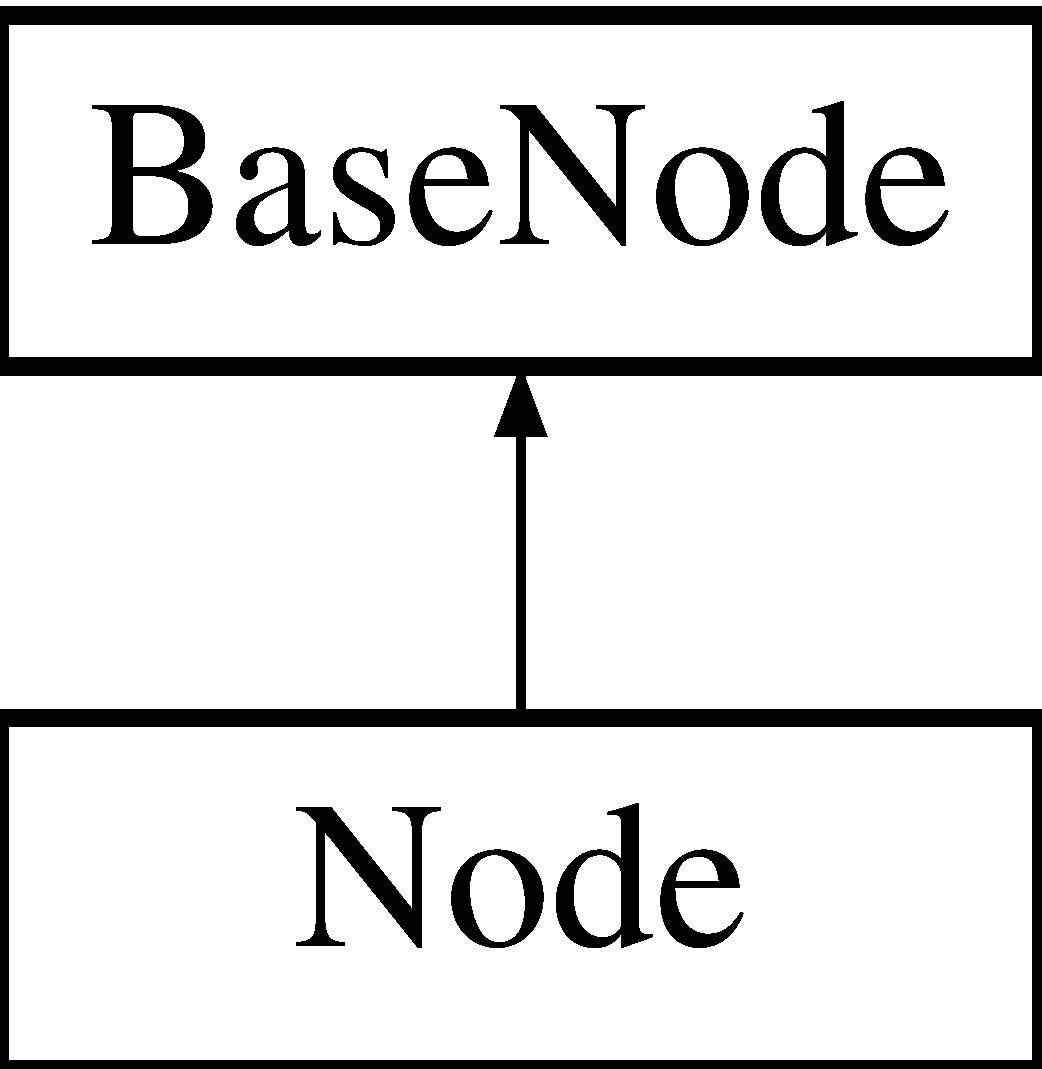
\includegraphics[height=2.000000cm]{class_node}
\end{center}
\end{figure}
\subsection*{Public Member Functions}
\begin{DoxyCompactItemize}
\item 
\hyperlink{class_node_a8d9cf8575744ca8c0f236a0a82eda096}{Node} (void)
\item 
\hyperlink{class_node_a4bf5930c1238505203c3dcf6e4573bad}{Node} (const \hyperlink{class_node}{Node} \&node)
\item 
\hyperlink{class_node_a3bb0c374e940be9178df34ba5272f92f}{Node} (const \hyperlink{types_8h_a64b5be62be31dcda165d2c6c3c262fb5}{bytevector} data)
\item 
\hyperlink{class_node_acdaa8db8d24d95d0c92218036a2df7e9}{Node} (const std\-::string filename)
\item 
\hyperlink{class_node_ae7672b93ee7885c40047f2f2f66578c0}{Node} (std\-::istream \&file)
\item 
\hyperlink{class_node_a2ba9aa5f85c0511a0608435419d248d1}{$\sim$\-Node} (void)
\item 
virtual \hyperlink{types_8h_a64b5be62be31dcda165d2c6c3c262fb5}{bytevector} \hyperlink{class_node_a858d4b4757880eba1fdead1412418693}{to\-Vector} (void) const 
\item 
\hyperlink{class_node}{Node} \& \hyperlink{class_node_a443734765d4e94a04ef8a5cba4c2d3fe}{operator=} (const \hyperlink{class_node}{Node} \&node)
\item 
\hyperlink{class_node}{Node} \& \hyperlink{class_node_aaf0d06b7e27f852f325c63b88eb33cdd}{mod\-To} (const \hyperlink{class_int_leaf}{Int\-Leaf} \&leaf)
\item 
\hyperlink{class_node}{Node} \hyperlink{class_node_a7744980c6da2415c02b583c5b149d50d}{mod} (const \hyperlink{class_int_leaf}{Int\-Leaf} \&leaf) const 
\item 
\hyperlink{class_node}{Node} \& \hyperlink{class_node_a6ca8cd41ea9f7579064f0c5ab4ae4ecf}{add\-To} (const \hyperlink{class_int_leaf}{Int\-Leaf} \&leaf)
\item 
\hyperlink{class_node}{Node} \hyperlink{class_node_ab3a58067bedece32403988a558ccbf96}{add} (const \hyperlink{class_int_leaf}{Int\-Leaf} \&leaf) const 
\item 
\hyperlink{class_node}{Node} \& \hyperlink{class_node_a7fc4be898d3ddebdc1a7341cc89a27f2}{add\-To} (const \hyperlink{class_node}{Node} \&node)
\item 
\hyperlink{class_node}{Node} \hyperlink{class_node_a162d4484dacf7c47d4e0bc13d3d29237}{add} (const \hyperlink{class_node}{Node} \&node) const 
\item 
\hyperlink{class_node}{Node} \& \hyperlink{class_node_ab11fa7ff8a60506e6bb40d63e8915cc4}{add\-To\-Mod} (const \hyperlink{class_int_leaf}{Int\-Leaf} \&leaf, const \hyperlink{class_int_leaf}{Int\-Leaf} \&\hyperlink{class_node_a7744980c6da2415c02b583c5b149d50d}{mod})
\item 
\hyperlink{class_node}{Node} \hyperlink{class_node_acfacf729f89f5323b6e1b84068f9af9e}{add\-Mod} (const \hyperlink{class_int_leaf}{Int\-Leaf} \&leaf, const \hyperlink{class_int_leaf}{Int\-Leaf} \&\hyperlink{class_node_a7744980c6da2415c02b583c5b149d50d}{mod}) const 
\item 
\hyperlink{class_node}{Node} \& \hyperlink{class_node_aeb43d1eb8c37653b358a6b10146830d5}{add\-To\-Mod} (const \hyperlink{class_node}{Node} \&node, const \hyperlink{class_int_leaf}{Int\-Leaf} \&\hyperlink{class_node_a7744980c6da2415c02b583c5b149d50d}{mod})
\item 
\hyperlink{class_node}{Node} \hyperlink{class_node_a7e486eaa03af545ab88e073ff66ade72}{add\-Mod} (const \hyperlink{class_node}{Node} \&node, const \hyperlink{class_int_leaf}{Int\-Leaf} \&\hyperlink{class_node_a7744980c6da2415c02b583c5b149d50d}{mod}) const 
\item 
\hyperlink{class_node}{Node} \& \hyperlink{class_node_a93ad5163448f65efe9ff4f816620ce15}{operator+=} (const \hyperlink{class_int_leaf}{Int\-Leaf} \&leaf)
\item 
\hyperlink{class_node}{Node} \hyperlink{class_node_a760ed8d9512bcdbd1d2c50a1e9db0c88}{operator+} (const \hyperlink{class_int_leaf}{Int\-Leaf} \&leaf) const 
\item 
\hyperlink{class_node}{Node} \& \hyperlink{class_node_aefaf03590fe3f94039db698524a263fe}{operator+=} (const \hyperlink{class_node}{Node} \&node)
\item 
\hyperlink{class_node}{Node} \hyperlink{class_node_ab340f7a5d7aef6d514c83378c1af3bb9}{operator+} (const \hyperlink{class_node}{Node} \&node) const 
\item 
\hyperlink{class_node}{Node} \& \hyperlink{class_node_a80101b65aa4de587b00ebe31c377e0d8}{mult\-To} (const \hyperlink{class_int_leaf}{Int\-Leaf} \&leaf)
\item 
\hyperlink{class_node}{Node} \hyperlink{class_node_aa975fa8176089de17add587ab9dc2f67}{mult} (const \hyperlink{class_int_leaf}{Int\-Leaf} \&leaf) const 
\item 
\hyperlink{class_node}{Node} \& \hyperlink{class_node_ae3250c7847ec855bd8b30105e60349c4}{mult\-To} (const \hyperlink{class_node}{Node} \&node)
\item 
\hyperlink{class_node}{Node} \hyperlink{class_node_a22afe59e2c925924d6472a6ffe3e5488}{mult} (const \hyperlink{class_node}{Node} \&node) const 
\item 
\hyperlink{class_node}{Node} \& \hyperlink{class_node_a24f08a59947b6ef5393823ddb47d5bde}{mult\-To\-Mod} (const \hyperlink{class_int_leaf}{Int\-Leaf} \&leaf, const \hyperlink{class_int_leaf}{Int\-Leaf} \&\hyperlink{class_node_a7744980c6da2415c02b583c5b149d50d}{mod})
\item 
\hyperlink{class_node}{Node} \hyperlink{class_node_a4e4c3d8ce4cd291c80b34a57eccdcfbc}{mult\-Mod} (const \hyperlink{class_int_leaf}{Int\-Leaf} \&leaf, const \hyperlink{class_int_leaf}{Int\-Leaf} \&\hyperlink{class_node_a7744980c6da2415c02b583c5b149d50d}{mod}) const 
\item 
\hyperlink{class_node}{Node} \& \hyperlink{class_node_a8a8d36cdd28616c89c5231f64eccb88b}{mult\-To\-Mod} (const \hyperlink{class_node}{Node} \&node, const \hyperlink{class_int_leaf}{Int\-Leaf} \&\hyperlink{class_node_a7744980c6da2415c02b583c5b149d50d}{mod})
\item 
\hyperlink{class_node}{Node} \hyperlink{class_node_add4a910a5d13cb0c43680de2e38d5758}{mult\-Mod} (const \hyperlink{class_node}{Node} \&node, const \hyperlink{class_int_leaf}{Int\-Leaf} \&\hyperlink{class_node_a7744980c6da2415c02b583c5b149d50d}{mod}) const 
\item 
\hyperlink{class_node}{Node} \& \hyperlink{class_node_acc1124101cc3bb6cfa486361d4593ef9}{operator$\ast$=} (const \hyperlink{class_int_leaf}{Int\-Leaf} \&leaf)
\item 
\hyperlink{class_node}{Node} \hyperlink{class_node_abf463388fe626c7412ebd03455b93d24}{operator$\ast$} (const \hyperlink{class_int_leaf}{Int\-Leaf} \&leaf) const 
\item 
\hyperlink{class_node}{Node} \& \hyperlink{class_node_a82be68d29507f13cd58d7a70678c745d}{operator$\ast$=} (const \hyperlink{class_node}{Node} \&node)
\item 
\hyperlink{class_node}{Node} \hyperlink{class_node_a74005185f7ea1724fb4891cd9df1e9ef}{operator$\ast$} (const \hyperlink{class_node}{Node} \&node) const 
\item 
bool \hyperlink{class_node_af167bfaab0f7e39daf0f39bb3d595e5f}{operator==} (const \hyperlink{class_node}{Node} \&node) const 
\item 
bool \hyperlink{class_node_aa2e7398fc0d99fe12c075bd94ee5543b}{operator!=} (const \hyperlink{class_node}{Node} \&node) const 
\item 
\hyperlink{class_int_leaf}{Int\-Leaf} \hyperlink{class_node_ac2103aa6d114e52dce1743be7aa4c1d0}{sum} (void) const 
\item 
\hyperlink{class_int_leaf}{Int\-Leaf} \hyperlink{class_node_ab70ce6887d26a52ff54bbc96bb79b7a4}{sum\-Mod} (const \hyperlink{class_int_leaf}{Int\-Leaf} \&\hyperlink{class_node_a7744980c6da2415c02b583c5b149d50d}{mod}) const 
\item 
\hyperlink{class_int_leaf}{Int\-Leaf} \hyperlink{class_node_ae2b74409d1e5040d11890cfae5a1713c}{prod} (void) const 
\item 
\hyperlink{class_int_leaf}{Int\-Leaf} \hyperlink{class_node_af18b21646a0a3e08690de85ffb1d3355}{prod\-Mod} (const \hyperlink{class_int_leaf}{Int\-Leaf} \&\hyperlink{class_node_a7744980c6da2415c02b583c5b149d50d}{mod}) const 
\item 
\hyperlink{class_node}{Node} \hyperlink{class_node_a675af8768a53b4c55dde07ba3ee4e335}{exp} (unsigned long exponent) const 
\item 
\hyperlink{class_node}{Node} \hyperlink{class_node_a2cf5726aef85163ee34aff6f953897fe}{exp\-Mod} (unsigned long exponent, const \hyperlink{class_int_leaf}{Int\-Leaf} \&\hyperlink{class_node_a7744980c6da2415c02b583c5b149d50d}{mod}) const 
\item 
\hyperlink{class_node}{Node} \hyperlink{class_node_ad01843ea664f09880c82a949e094a107}{exp\-Mod} (const \hyperlink{class_int_leaf}{Int\-Leaf} \&exponent, const \hyperlink{class_int_leaf}{Int\-Leaf} \&\hyperlink{class_node_a7744980c6da2415c02b583c5b149d50d}{mod}) const 
\item 
\hyperlink{class_node}{Node} \hyperlink{class_node_af49a45863e320ed7b81ff96e4e35a73e}{exp} (const \hyperlink{class_node}{Node} \&exponents) const 
\item 
\hyperlink{class_node}{Node} \hyperlink{class_node_a270a6b9f196218ae688e34ec969f465f}{exp\-Mod} (const \hyperlink{class_node}{Node} \&exponents, const \hyperlink{class_int_leaf}{Int\-Leaf} \&\hyperlink{class_node_a7744980c6da2415c02b583c5b149d50d}{mod}) const 
\item 
\hyperlink{class_node}{Node} \& \hyperlink{class_node_a57700c1125aaf77210924a2acc128f48}{exp\-To} (unsigned long exponent)
\item 
\hyperlink{class_node}{Node} \& \hyperlink{class_node_a430517fa1163f53df68e9be38288dcd6}{exp\-To\-Mod} (unsigned long exponent, const \hyperlink{class_int_leaf}{Int\-Leaf} \&\hyperlink{class_node_a7744980c6da2415c02b583c5b149d50d}{mod})
\item 
\hyperlink{class_node}{Node} \& \hyperlink{class_node_afc7a7735704c514be511d52880a7c94c}{exp\-To\-Mod} (const \hyperlink{class_int_leaf}{Int\-Leaf} \&exponent, const \hyperlink{class_int_leaf}{Int\-Leaf} \&\hyperlink{class_node_a7744980c6da2415c02b583c5b149d50d}{mod})
\item 
\hyperlink{class_node}{Node} \& \hyperlink{class_node_a46ae5ee5f73f4f55b1600e93bc45c7f4}{exp\-To} (const \hyperlink{class_node}{Node} \&exponents)
\item 
\hyperlink{class_node}{Node} \& \hyperlink{class_node_aee8354142d2faea6f6e78f2d9dd321c0}{exp\-To\-Mod} (const \hyperlink{class_node}{Node} \&exponents, const \hyperlink{class_int_leaf}{Int\-Leaf} \&\hyperlink{class_node_a7744980c6da2415c02b583c5b149d50d}{mod})
\item 
\hyperlink{class_int_leaf}{Int\-Leaf} \hyperlink{class_node_af65555e953a065f650ff875bac1e3c27}{exp\-Mult\-Mod} (const \hyperlink{class_node}{Node} \&node, const \hyperlink{class_int_leaf}{Int\-Leaf} \&\hyperlink{class_node_a7744980c6da2415c02b583c5b149d50d}{mod}) const 
\item 
\hyperlink{class_int_leaf}{Int\-Leaf} \hyperlink{class_node_aaaddaae51a5f69c834919ebe9bc6e9e1}{exp\-Mult} (unsigned long exponent) const 
\item 
\hyperlink{class_int_leaf}{Int\-Leaf} \hyperlink{class_node_afbf297207f1366bdd0c279d89425b305}{exp\-Mult\-Mod} (unsigned long exponent, const \hyperlink{class_int_leaf}{Int\-Leaf} \&\hyperlink{class_node_a7744980c6da2415c02b583c5b149d50d}{mod}) const 
\item 
\hyperlink{class_node}{Node} \& \hyperlink{class_node_a9b098b18df4102d4e8bcce7114c389ea}{add\-Child} (const \hyperlink{class_base_node}{Base\-Node} \&child)
\item 
\hyperlink{class_node}{Node} \hyperlink{class_node_a3932c819906609e93ee189946f658d8d}{get\-Children} (int32\-\_\-t index) const 
\item 
\hyperlink{class_int_leaf}{Int\-Leaf} \& \hyperlink{class_node_a4fd5db27b06140e0421565c2b21c3973}{get\-Int\-Leaf\-Child} (int32\-\_\-t index)
\item 
const \hyperlink{class_int_leaf}{Int\-Leaf} \& \hyperlink{class_node_acf7ea79479333bee29105efe5d8fa663}{get\-Int\-Leaf\-Child} (int32\-\_\-t index) const 
\item 
\hyperlink{class_node}{Node} \& \hyperlink{class_node_a5379035c4d7e6080e40e57bb72e2e761}{get\-Node\-Child} (int32\-\_\-t index)
\item 
const \hyperlink{class_node}{Node} \& \hyperlink{class_node_a161add6a6b67043ce1fc5a7b7c9bee87}{get\-Node\-Child} (int32\-\_\-t index) const 
\item 
std\-::string \hyperlink{class_node_a1b0277500ee7e1019fc5d69d19071303}{to\-String} (void) const 
\item 
virtual int32\-\_\-t \hyperlink{class_node_ad602104b3c245a564f741b65fe97845c}{get\-Length} (void) const 
\end{DoxyCompactItemize}
\subsection*{Static Public Member Functions}
\begin{DoxyCompactItemize}
\item 
static \hyperlink{class_base_node}{Base\-Node} $\ast$ \hyperlink{class_node_a2b43c8e76e3dd008affda12607770a62}{construct\-Part\-From\-File} (std\-::istream \&file, uint32\-\_\-t count)
\end{DoxyCompactItemize}
\subsection*{Additional Inherited Members}


\subsection{Constructor \& Destructor Documentation}
\hypertarget{class_node_a8d9cf8575744ca8c0f236a0a82eda096}{\index{Node@{Node}!Node@{Node}}
\index{Node@{Node}!Node@{Node}}
\subsubsection[{Node}]{\setlength{\rightskip}{0pt plus 5cm}Node\-::\-Node (
\begin{DoxyParamCaption}
\item[{void}]{}
\end{DoxyParamCaption}
)}}\label{class_node_a8d9cf8575744ca8c0f236a0a82eda096}
\hypertarget{class_node_a4bf5930c1238505203c3dcf6e4573bad}{\index{Node@{Node}!Node@{Node}}
\index{Node@{Node}!Node@{Node}}
\subsubsection[{Node}]{\setlength{\rightskip}{0pt plus 5cm}Node\-::\-Node (
\begin{DoxyParamCaption}
\item[{const {\bf Node} \&}]{node}
\end{DoxyParamCaption}
)}}\label{class_node_a4bf5930c1238505203c3dcf6e4573bad}
\hypertarget{class_node_a3bb0c374e940be9178df34ba5272f92f}{\index{Node@{Node}!Node@{Node}}
\index{Node@{Node}!Node@{Node}}
\subsubsection[{Node}]{\setlength{\rightskip}{0pt plus 5cm}Node\-::\-Node (
\begin{DoxyParamCaption}
\item[{const {\bf bytevector}}]{data}
\end{DoxyParamCaption}
)}}\label{class_node_a3bb0c374e940be9178df34ba5272f92f}
\hypertarget{class_node_acdaa8db8d24d95d0c92218036a2df7e9}{\index{Node@{Node}!Node@{Node}}
\index{Node@{Node}!Node@{Node}}
\subsubsection[{Node}]{\setlength{\rightskip}{0pt plus 5cm}Node\-::\-Node (
\begin{DoxyParamCaption}
\item[{const std\-::string}]{filename}
\end{DoxyParamCaption}
)\hspace{0.3cm}{\ttfamily [explicit]}}}\label{class_node_acdaa8db8d24d95d0c92218036a2df7e9}
\hypertarget{class_node_ae7672b93ee7885c40047f2f2f66578c0}{\index{Node@{Node}!Node@{Node}}
\index{Node@{Node}!Node@{Node}}
\subsubsection[{Node}]{\setlength{\rightskip}{0pt plus 5cm}Node\-::\-Node (
\begin{DoxyParamCaption}
\item[{std\-::istream \&}]{file}
\end{DoxyParamCaption}
)\hspace{0.3cm}{\ttfamily [explicit]}}}\label{class_node_ae7672b93ee7885c40047f2f2f66578c0}
\hypertarget{class_node_a2ba9aa5f85c0511a0608435419d248d1}{\index{Node@{Node}!$\sim$\-Node@{$\sim$\-Node}}
\index{$\sim$\-Node@{$\sim$\-Node}!Node@{Node}}
\subsubsection[{$\sim$\-Node}]{\setlength{\rightskip}{0pt plus 5cm}Node\-::$\sim$\-Node (
\begin{DoxyParamCaption}
\item[{void}]{}
\end{DoxyParamCaption}
)}}\label{class_node_a2ba9aa5f85c0511a0608435419d248d1}


\subsection{Member Function Documentation}
\hypertarget{class_node_ab3a58067bedece32403988a558ccbf96}{\index{Node@{Node}!add@{add}}
\index{add@{add}!Node@{Node}}
\subsubsection[{add}]{\setlength{\rightskip}{0pt plus 5cm}{\bf Node} Node\-::add (
\begin{DoxyParamCaption}
\item[{const {\bf Int\-Leaf} \&}]{leaf}
\end{DoxyParamCaption}
) const}}\label{class_node_ab3a58067bedece32403988a558ccbf96}
\hypertarget{class_node_a162d4484dacf7c47d4e0bc13d3d29237}{\index{Node@{Node}!add@{add}}
\index{add@{add}!Node@{Node}}
\subsubsection[{add}]{\setlength{\rightskip}{0pt plus 5cm}{\bf Node} Node\-::add (
\begin{DoxyParamCaption}
\item[{const {\bf Node} \&}]{node}
\end{DoxyParamCaption}
) const}}\label{class_node_a162d4484dacf7c47d4e0bc13d3d29237}
\hypertarget{class_node_a9b098b18df4102d4e8bcce7114c389ea}{\index{Node@{Node}!add\-Child@{add\-Child}}
\index{add\-Child@{add\-Child}!Node@{Node}}
\subsubsection[{add\-Child}]{\setlength{\rightskip}{0pt plus 5cm}{\bf Node} \& Node\-::add\-Child (
\begin{DoxyParamCaption}
\item[{const {\bf Base\-Node} \&}]{child}
\end{DoxyParamCaption}
)}}\label{class_node_a9b098b18df4102d4e8bcce7114c389ea}
\hypertarget{class_node_acfacf729f89f5323b6e1b84068f9af9e}{\index{Node@{Node}!add\-Mod@{add\-Mod}}
\index{add\-Mod@{add\-Mod}!Node@{Node}}
\subsubsection[{add\-Mod}]{\setlength{\rightskip}{0pt plus 5cm}{\bf Node} Node\-::add\-Mod (
\begin{DoxyParamCaption}
\item[{const {\bf Int\-Leaf} \&}]{leaf, }
\item[{const {\bf Int\-Leaf} \&}]{mod}
\end{DoxyParamCaption}
) const}}\label{class_node_acfacf729f89f5323b6e1b84068f9af9e}
\hypertarget{class_node_a7e486eaa03af545ab88e073ff66ade72}{\index{Node@{Node}!add\-Mod@{add\-Mod}}
\index{add\-Mod@{add\-Mod}!Node@{Node}}
\subsubsection[{add\-Mod}]{\setlength{\rightskip}{0pt plus 5cm}{\bf Node} Node\-::add\-Mod (
\begin{DoxyParamCaption}
\item[{const {\bf Node} \&}]{node, }
\item[{const {\bf Int\-Leaf} \&}]{mod}
\end{DoxyParamCaption}
) const}}\label{class_node_a7e486eaa03af545ab88e073ff66ade72}
\hypertarget{class_node_a6ca8cd41ea9f7579064f0c5ab4ae4ecf}{\index{Node@{Node}!add\-To@{add\-To}}
\index{add\-To@{add\-To}!Node@{Node}}
\subsubsection[{add\-To}]{\setlength{\rightskip}{0pt plus 5cm}{\bf Node} \& Node\-::add\-To (
\begin{DoxyParamCaption}
\item[{const {\bf Int\-Leaf} \&}]{leaf}
\end{DoxyParamCaption}
)}}\label{class_node_a6ca8cd41ea9f7579064f0c5ab4ae4ecf}
\hypertarget{class_node_a7fc4be898d3ddebdc1a7341cc89a27f2}{\index{Node@{Node}!add\-To@{add\-To}}
\index{add\-To@{add\-To}!Node@{Node}}
\subsubsection[{add\-To}]{\setlength{\rightskip}{0pt plus 5cm}{\bf Node} \& Node\-::add\-To (
\begin{DoxyParamCaption}
\item[{const {\bf Node} \&}]{node}
\end{DoxyParamCaption}
)}}\label{class_node_a7fc4be898d3ddebdc1a7341cc89a27f2}
\hypertarget{class_node_ab11fa7ff8a60506e6bb40d63e8915cc4}{\index{Node@{Node}!add\-To\-Mod@{add\-To\-Mod}}
\index{add\-To\-Mod@{add\-To\-Mod}!Node@{Node}}
\subsubsection[{add\-To\-Mod}]{\setlength{\rightskip}{0pt plus 5cm}{\bf Node} \& Node\-::add\-To\-Mod (
\begin{DoxyParamCaption}
\item[{const {\bf Int\-Leaf} \&}]{leaf, }
\item[{const {\bf Int\-Leaf} \&}]{mod}
\end{DoxyParamCaption}
)}}\label{class_node_ab11fa7ff8a60506e6bb40d63e8915cc4}
\hypertarget{class_node_aeb43d1eb8c37653b358a6b10146830d5}{\index{Node@{Node}!add\-To\-Mod@{add\-To\-Mod}}
\index{add\-To\-Mod@{add\-To\-Mod}!Node@{Node}}
\subsubsection[{add\-To\-Mod}]{\setlength{\rightskip}{0pt plus 5cm}{\bf Node} \& Node\-::add\-To\-Mod (
\begin{DoxyParamCaption}
\item[{const {\bf Node} \&}]{node, }
\item[{const {\bf Int\-Leaf} \&}]{mod}
\end{DoxyParamCaption}
)}}\label{class_node_aeb43d1eb8c37653b358a6b10146830d5}
\hypertarget{class_node_a2b43c8e76e3dd008affda12607770a62}{\index{Node@{Node}!construct\-Part\-From\-File@{construct\-Part\-From\-File}}
\index{construct\-Part\-From\-File@{construct\-Part\-From\-File}!Node@{Node}}
\subsubsection[{construct\-Part\-From\-File}]{\setlength{\rightskip}{0pt plus 5cm}{\bf Base\-Node} $\ast$ Node\-::construct\-Part\-From\-File (
\begin{DoxyParamCaption}
\item[{std\-::istream \&}]{file, }
\item[{uint32\-\_\-t}]{count}
\end{DoxyParamCaption}
)\hspace{0.3cm}{\ttfamily [static]}}}\label{class_node_a2b43c8e76e3dd008affda12607770a62}
\hypertarget{class_node_a675af8768a53b4c55dde07ba3ee4e335}{\index{Node@{Node}!exp@{exp}}
\index{exp@{exp}!Node@{Node}}
\subsubsection[{exp}]{\setlength{\rightskip}{0pt plus 5cm}{\bf Node} Node\-::exp (
\begin{DoxyParamCaption}
\item[{unsigned long}]{exponent}
\end{DoxyParamCaption}
) const}}\label{class_node_a675af8768a53b4c55dde07ba3ee4e335}
\hypertarget{class_node_af49a45863e320ed7b81ff96e4e35a73e}{\index{Node@{Node}!exp@{exp}}
\index{exp@{exp}!Node@{Node}}
\subsubsection[{exp}]{\setlength{\rightskip}{0pt plus 5cm}{\bf Node} Node\-::exp (
\begin{DoxyParamCaption}
\item[{const {\bf Node} \&}]{exponents}
\end{DoxyParamCaption}
) const}}\label{class_node_af49a45863e320ed7b81ff96e4e35a73e}
\hypertarget{class_node_a2cf5726aef85163ee34aff6f953897fe}{\index{Node@{Node}!exp\-Mod@{exp\-Mod}}
\index{exp\-Mod@{exp\-Mod}!Node@{Node}}
\subsubsection[{exp\-Mod}]{\setlength{\rightskip}{0pt plus 5cm}{\bf Node} Node\-::exp\-Mod (
\begin{DoxyParamCaption}
\item[{unsigned long}]{exponent, }
\item[{const {\bf Int\-Leaf} \&}]{mod}
\end{DoxyParamCaption}
) const}}\label{class_node_a2cf5726aef85163ee34aff6f953897fe}
\hypertarget{class_node_ad01843ea664f09880c82a949e094a107}{\index{Node@{Node}!exp\-Mod@{exp\-Mod}}
\index{exp\-Mod@{exp\-Mod}!Node@{Node}}
\subsubsection[{exp\-Mod}]{\setlength{\rightskip}{0pt plus 5cm}{\bf Node} Node\-::exp\-Mod (
\begin{DoxyParamCaption}
\item[{const {\bf Int\-Leaf} \&}]{exponent, }
\item[{const {\bf Int\-Leaf} \&}]{mod}
\end{DoxyParamCaption}
) const}}\label{class_node_ad01843ea664f09880c82a949e094a107}
\hypertarget{class_node_a270a6b9f196218ae688e34ec969f465f}{\index{Node@{Node}!exp\-Mod@{exp\-Mod}}
\index{exp\-Mod@{exp\-Mod}!Node@{Node}}
\subsubsection[{exp\-Mod}]{\setlength{\rightskip}{0pt plus 5cm}{\bf Node} Node\-::exp\-Mod (
\begin{DoxyParamCaption}
\item[{const {\bf Node} \&}]{exponents, }
\item[{const {\bf Int\-Leaf} \&}]{mod}
\end{DoxyParamCaption}
) const}}\label{class_node_a270a6b9f196218ae688e34ec969f465f}
\hypertarget{class_node_aaaddaae51a5f69c834919ebe9bc6e9e1}{\index{Node@{Node}!exp\-Mult@{exp\-Mult}}
\index{exp\-Mult@{exp\-Mult}!Node@{Node}}
\subsubsection[{exp\-Mult}]{\setlength{\rightskip}{0pt plus 5cm}{\bf Int\-Leaf} Node\-::exp\-Mult (
\begin{DoxyParamCaption}
\item[{unsigned long}]{exponent}
\end{DoxyParamCaption}
) const}}\label{class_node_aaaddaae51a5f69c834919ebe9bc6e9e1}
\hypertarget{class_node_af65555e953a065f650ff875bac1e3c27}{\index{Node@{Node}!exp\-Mult\-Mod@{exp\-Mult\-Mod}}
\index{exp\-Mult\-Mod@{exp\-Mult\-Mod}!Node@{Node}}
\subsubsection[{exp\-Mult\-Mod}]{\setlength{\rightskip}{0pt plus 5cm}{\bf Int\-Leaf} Node\-::exp\-Mult\-Mod (
\begin{DoxyParamCaption}
\item[{const {\bf Node} \&}]{node, }
\item[{const {\bf Int\-Leaf} \&}]{mod}
\end{DoxyParamCaption}
) const}}\label{class_node_af65555e953a065f650ff875bac1e3c27}
\hypertarget{class_node_afbf297207f1366bdd0c279d89425b305}{\index{Node@{Node}!exp\-Mult\-Mod@{exp\-Mult\-Mod}}
\index{exp\-Mult\-Mod@{exp\-Mult\-Mod}!Node@{Node}}
\subsubsection[{exp\-Mult\-Mod}]{\setlength{\rightskip}{0pt plus 5cm}{\bf Int\-Leaf} Node\-::exp\-Mult\-Mod (
\begin{DoxyParamCaption}
\item[{unsigned long}]{exponent, }
\item[{const {\bf Int\-Leaf} \&}]{mod}
\end{DoxyParamCaption}
) const}}\label{class_node_afbf297207f1366bdd0c279d89425b305}
\hypertarget{class_node_a57700c1125aaf77210924a2acc128f48}{\index{Node@{Node}!exp\-To@{exp\-To}}
\index{exp\-To@{exp\-To}!Node@{Node}}
\subsubsection[{exp\-To}]{\setlength{\rightskip}{0pt plus 5cm}{\bf Node} \& Node\-::exp\-To (
\begin{DoxyParamCaption}
\item[{unsigned long}]{exponent}
\end{DoxyParamCaption}
)}}\label{class_node_a57700c1125aaf77210924a2acc128f48}
\hypertarget{class_node_a46ae5ee5f73f4f55b1600e93bc45c7f4}{\index{Node@{Node}!exp\-To@{exp\-To}}
\index{exp\-To@{exp\-To}!Node@{Node}}
\subsubsection[{exp\-To}]{\setlength{\rightskip}{0pt plus 5cm}{\bf Node}\& Node\-::exp\-To (
\begin{DoxyParamCaption}
\item[{const {\bf Node} \&}]{exponents}
\end{DoxyParamCaption}
)}}\label{class_node_a46ae5ee5f73f4f55b1600e93bc45c7f4}
\hypertarget{class_node_a430517fa1163f53df68e9be38288dcd6}{\index{Node@{Node}!exp\-To\-Mod@{exp\-To\-Mod}}
\index{exp\-To\-Mod@{exp\-To\-Mod}!Node@{Node}}
\subsubsection[{exp\-To\-Mod}]{\setlength{\rightskip}{0pt plus 5cm}{\bf Node} \& Node\-::exp\-To\-Mod (
\begin{DoxyParamCaption}
\item[{unsigned long}]{exponent, }
\item[{const {\bf Int\-Leaf} \&}]{mod}
\end{DoxyParamCaption}
)}}\label{class_node_a430517fa1163f53df68e9be38288dcd6}
\hypertarget{class_node_afc7a7735704c514be511d52880a7c94c}{\index{Node@{Node}!exp\-To\-Mod@{exp\-To\-Mod}}
\index{exp\-To\-Mod@{exp\-To\-Mod}!Node@{Node}}
\subsubsection[{exp\-To\-Mod}]{\setlength{\rightskip}{0pt plus 5cm}{\bf Node} \& Node\-::exp\-To\-Mod (
\begin{DoxyParamCaption}
\item[{const {\bf Int\-Leaf} \&}]{exponent, }
\item[{const {\bf Int\-Leaf} \&}]{mod}
\end{DoxyParamCaption}
)}}\label{class_node_afc7a7735704c514be511d52880a7c94c}
\hypertarget{class_node_aee8354142d2faea6f6e78f2d9dd321c0}{\index{Node@{Node}!exp\-To\-Mod@{exp\-To\-Mod}}
\index{exp\-To\-Mod@{exp\-To\-Mod}!Node@{Node}}
\subsubsection[{exp\-To\-Mod}]{\setlength{\rightskip}{0pt plus 5cm}{\bf Node}\& Node\-::exp\-To\-Mod (
\begin{DoxyParamCaption}
\item[{const {\bf Node} \&}]{exponents, }
\item[{const {\bf Int\-Leaf} \&}]{mod}
\end{DoxyParamCaption}
)}}\label{class_node_aee8354142d2faea6f6e78f2d9dd321c0}
\hypertarget{class_node_a3932c819906609e93ee189946f658d8d}{\index{Node@{Node}!get\-Children@{get\-Children}}
\index{get\-Children@{get\-Children}!Node@{Node}}
\subsubsection[{get\-Children}]{\setlength{\rightskip}{0pt plus 5cm}{\bf Node} Node\-::get\-Children (
\begin{DoxyParamCaption}
\item[{int32\-\_\-t}]{index}
\end{DoxyParamCaption}
) const}}\label{class_node_a3932c819906609e93ee189946f658d8d}
\hypertarget{class_node_a4fd5db27b06140e0421565c2b21c3973}{\index{Node@{Node}!get\-Int\-Leaf\-Child@{get\-Int\-Leaf\-Child}}
\index{get\-Int\-Leaf\-Child@{get\-Int\-Leaf\-Child}!Node@{Node}}
\subsubsection[{get\-Int\-Leaf\-Child}]{\setlength{\rightskip}{0pt plus 5cm}{\bf Int\-Leaf} \& Node\-::get\-Int\-Leaf\-Child (
\begin{DoxyParamCaption}
\item[{int32\-\_\-t}]{index}
\end{DoxyParamCaption}
)}}\label{class_node_a4fd5db27b06140e0421565c2b21c3973}
\hypertarget{class_node_acf7ea79479333bee29105efe5d8fa663}{\index{Node@{Node}!get\-Int\-Leaf\-Child@{get\-Int\-Leaf\-Child}}
\index{get\-Int\-Leaf\-Child@{get\-Int\-Leaf\-Child}!Node@{Node}}
\subsubsection[{get\-Int\-Leaf\-Child}]{\setlength{\rightskip}{0pt plus 5cm}const {\bf Int\-Leaf} \& Node\-::get\-Int\-Leaf\-Child (
\begin{DoxyParamCaption}
\item[{int32\-\_\-t}]{index}
\end{DoxyParamCaption}
) const}}\label{class_node_acf7ea79479333bee29105efe5d8fa663}
\hypertarget{class_node_ad602104b3c245a564f741b65fe97845c}{\index{Node@{Node}!get\-Length@{get\-Length}}
\index{get\-Length@{get\-Length}!Node@{Node}}
\subsubsection[{get\-Length}]{\setlength{\rightskip}{0pt plus 5cm}int32\-\_\-t Node\-::get\-Length (
\begin{DoxyParamCaption}
\item[{void}]{}
\end{DoxyParamCaption}
) const\hspace{0.3cm}{\ttfamily [virtual]}}}\label{class_node_ad602104b3c245a564f741b65fe97845c}


Implements \hyperlink{class_base_node_a50aef77f988f7689e96b346705628f91}{Base\-Node}.

\hypertarget{class_node_a5379035c4d7e6080e40e57bb72e2e761}{\index{Node@{Node}!get\-Node\-Child@{get\-Node\-Child}}
\index{get\-Node\-Child@{get\-Node\-Child}!Node@{Node}}
\subsubsection[{get\-Node\-Child}]{\setlength{\rightskip}{0pt plus 5cm}{\bf Node} \& Node\-::get\-Node\-Child (
\begin{DoxyParamCaption}
\item[{int32\-\_\-t}]{index}
\end{DoxyParamCaption}
)}}\label{class_node_a5379035c4d7e6080e40e57bb72e2e761}
\hypertarget{class_node_a161add6a6b67043ce1fc5a7b7c9bee87}{\index{Node@{Node}!get\-Node\-Child@{get\-Node\-Child}}
\index{get\-Node\-Child@{get\-Node\-Child}!Node@{Node}}
\subsubsection[{get\-Node\-Child}]{\setlength{\rightskip}{0pt plus 5cm}const {\bf Node} \& Node\-::get\-Node\-Child (
\begin{DoxyParamCaption}
\item[{int32\-\_\-t}]{index}
\end{DoxyParamCaption}
) const}}\label{class_node_a161add6a6b67043ce1fc5a7b7c9bee87}
\hypertarget{class_node_a7744980c6da2415c02b583c5b149d50d}{\index{Node@{Node}!mod@{mod}}
\index{mod@{mod}!Node@{Node}}
\subsubsection[{mod}]{\setlength{\rightskip}{0pt plus 5cm}{\bf Node} Node\-::mod (
\begin{DoxyParamCaption}
\item[{const {\bf Int\-Leaf} \&}]{leaf}
\end{DoxyParamCaption}
) const}}\label{class_node_a7744980c6da2415c02b583c5b149d50d}
\hypertarget{class_node_aaf0d06b7e27f852f325c63b88eb33cdd}{\index{Node@{Node}!mod\-To@{mod\-To}}
\index{mod\-To@{mod\-To}!Node@{Node}}
\subsubsection[{mod\-To}]{\setlength{\rightskip}{0pt plus 5cm}{\bf Node} \& Node\-::mod\-To (
\begin{DoxyParamCaption}
\item[{const {\bf Int\-Leaf} \&}]{leaf}
\end{DoxyParamCaption}
)}}\label{class_node_aaf0d06b7e27f852f325c63b88eb33cdd}
\hypertarget{class_node_aa975fa8176089de17add587ab9dc2f67}{\index{Node@{Node}!mult@{mult}}
\index{mult@{mult}!Node@{Node}}
\subsubsection[{mult}]{\setlength{\rightskip}{0pt plus 5cm}{\bf Node} Node\-::mult (
\begin{DoxyParamCaption}
\item[{const {\bf Int\-Leaf} \&}]{leaf}
\end{DoxyParamCaption}
) const}}\label{class_node_aa975fa8176089de17add587ab9dc2f67}
\hypertarget{class_node_a22afe59e2c925924d6472a6ffe3e5488}{\index{Node@{Node}!mult@{mult}}
\index{mult@{mult}!Node@{Node}}
\subsubsection[{mult}]{\setlength{\rightskip}{0pt plus 5cm}{\bf Node} Node\-::mult (
\begin{DoxyParamCaption}
\item[{const {\bf Node} \&}]{node}
\end{DoxyParamCaption}
) const}}\label{class_node_a22afe59e2c925924d6472a6ffe3e5488}
\hypertarget{class_node_a4e4c3d8ce4cd291c80b34a57eccdcfbc}{\index{Node@{Node}!mult\-Mod@{mult\-Mod}}
\index{mult\-Mod@{mult\-Mod}!Node@{Node}}
\subsubsection[{mult\-Mod}]{\setlength{\rightskip}{0pt plus 5cm}{\bf Node} Node\-::mult\-Mod (
\begin{DoxyParamCaption}
\item[{const {\bf Int\-Leaf} \&}]{leaf, }
\item[{const {\bf Int\-Leaf} \&}]{mod}
\end{DoxyParamCaption}
) const}}\label{class_node_a4e4c3d8ce4cd291c80b34a57eccdcfbc}
\hypertarget{class_node_add4a910a5d13cb0c43680de2e38d5758}{\index{Node@{Node}!mult\-Mod@{mult\-Mod}}
\index{mult\-Mod@{mult\-Mod}!Node@{Node}}
\subsubsection[{mult\-Mod}]{\setlength{\rightskip}{0pt plus 5cm}{\bf Node} Node\-::mult\-Mod (
\begin{DoxyParamCaption}
\item[{const {\bf Node} \&}]{node, }
\item[{const {\bf Int\-Leaf} \&}]{mod}
\end{DoxyParamCaption}
) const}}\label{class_node_add4a910a5d13cb0c43680de2e38d5758}
\hypertarget{class_node_a80101b65aa4de587b00ebe31c377e0d8}{\index{Node@{Node}!mult\-To@{mult\-To}}
\index{mult\-To@{mult\-To}!Node@{Node}}
\subsubsection[{mult\-To}]{\setlength{\rightskip}{0pt plus 5cm}{\bf Node} \& Node\-::mult\-To (
\begin{DoxyParamCaption}
\item[{const {\bf Int\-Leaf} \&}]{leaf}
\end{DoxyParamCaption}
)}}\label{class_node_a80101b65aa4de587b00ebe31c377e0d8}
\hypertarget{class_node_ae3250c7847ec855bd8b30105e60349c4}{\index{Node@{Node}!mult\-To@{mult\-To}}
\index{mult\-To@{mult\-To}!Node@{Node}}
\subsubsection[{mult\-To}]{\setlength{\rightskip}{0pt plus 5cm}{\bf Node} \& Node\-::mult\-To (
\begin{DoxyParamCaption}
\item[{const {\bf Node} \&}]{node}
\end{DoxyParamCaption}
)}}\label{class_node_ae3250c7847ec855bd8b30105e60349c4}
\hypertarget{class_node_a24f08a59947b6ef5393823ddb47d5bde}{\index{Node@{Node}!mult\-To\-Mod@{mult\-To\-Mod}}
\index{mult\-To\-Mod@{mult\-To\-Mod}!Node@{Node}}
\subsubsection[{mult\-To\-Mod}]{\setlength{\rightskip}{0pt plus 5cm}{\bf Node} \& Node\-::mult\-To\-Mod (
\begin{DoxyParamCaption}
\item[{const {\bf Int\-Leaf} \&}]{leaf, }
\item[{const {\bf Int\-Leaf} \&}]{mod}
\end{DoxyParamCaption}
)}}\label{class_node_a24f08a59947b6ef5393823ddb47d5bde}
\hypertarget{class_node_a8a8d36cdd28616c89c5231f64eccb88b}{\index{Node@{Node}!mult\-To\-Mod@{mult\-To\-Mod}}
\index{mult\-To\-Mod@{mult\-To\-Mod}!Node@{Node}}
\subsubsection[{mult\-To\-Mod}]{\setlength{\rightskip}{0pt plus 5cm}{\bf Node} \& Node\-::mult\-To\-Mod (
\begin{DoxyParamCaption}
\item[{const {\bf Node} \&}]{node, }
\item[{const {\bf Int\-Leaf} \&}]{mod}
\end{DoxyParamCaption}
)}}\label{class_node_a8a8d36cdd28616c89c5231f64eccb88b}
\hypertarget{class_node_aa2e7398fc0d99fe12c075bd94ee5543b}{\index{Node@{Node}!operator!=@{operator!=}}
\index{operator!=@{operator!=}!Node@{Node}}
\subsubsection[{operator!=}]{\setlength{\rightskip}{0pt plus 5cm}bool Node\-::operator!= (
\begin{DoxyParamCaption}
\item[{const {\bf Node} \&}]{node}
\end{DoxyParamCaption}
) const}}\label{class_node_aa2e7398fc0d99fe12c075bd94ee5543b}
\hypertarget{class_node_abf463388fe626c7412ebd03455b93d24}{\index{Node@{Node}!operator$\ast$@{operator$\ast$}}
\index{operator$\ast$@{operator$\ast$}!Node@{Node}}
\subsubsection[{operator$\ast$}]{\setlength{\rightskip}{0pt plus 5cm}{\bf Node} Node\-::operator$\ast$ (
\begin{DoxyParamCaption}
\item[{const {\bf Int\-Leaf} \&}]{leaf}
\end{DoxyParamCaption}
) const}}\label{class_node_abf463388fe626c7412ebd03455b93d24}
\hypertarget{class_node_a74005185f7ea1724fb4891cd9df1e9ef}{\index{Node@{Node}!operator$\ast$@{operator$\ast$}}
\index{operator$\ast$@{operator$\ast$}!Node@{Node}}
\subsubsection[{operator$\ast$}]{\setlength{\rightskip}{0pt plus 5cm}{\bf Node} Node\-::operator$\ast$ (
\begin{DoxyParamCaption}
\item[{const {\bf Node} \&}]{node}
\end{DoxyParamCaption}
) const}}\label{class_node_a74005185f7ea1724fb4891cd9df1e9ef}
\hypertarget{class_node_acc1124101cc3bb6cfa486361d4593ef9}{\index{Node@{Node}!operator$\ast$=@{operator$\ast$=}}
\index{operator$\ast$=@{operator$\ast$=}!Node@{Node}}
\subsubsection[{operator$\ast$=}]{\setlength{\rightskip}{0pt plus 5cm}{\bf Node} \& Node\-::operator$\ast$= (
\begin{DoxyParamCaption}
\item[{const {\bf Int\-Leaf} \&}]{leaf}
\end{DoxyParamCaption}
)}}\label{class_node_acc1124101cc3bb6cfa486361d4593ef9}
\hypertarget{class_node_a82be68d29507f13cd58d7a70678c745d}{\index{Node@{Node}!operator$\ast$=@{operator$\ast$=}}
\index{operator$\ast$=@{operator$\ast$=}!Node@{Node}}
\subsubsection[{operator$\ast$=}]{\setlength{\rightskip}{0pt plus 5cm}{\bf Node} \& Node\-::operator$\ast$= (
\begin{DoxyParamCaption}
\item[{const {\bf Node} \&}]{node}
\end{DoxyParamCaption}
)}}\label{class_node_a82be68d29507f13cd58d7a70678c745d}
\hypertarget{class_node_a760ed8d9512bcdbd1d2c50a1e9db0c88}{\index{Node@{Node}!operator+@{operator+}}
\index{operator+@{operator+}!Node@{Node}}
\subsubsection[{operator+}]{\setlength{\rightskip}{0pt plus 5cm}{\bf Node} Node\-::operator+ (
\begin{DoxyParamCaption}
\item[{const {\bf Int\-Leaf} \&}]{leaf}
\end{DoxyParamCaption}
) const}}\label{class_node_a760ed8d9512bcdbd1d2c50a1e9db0c88}
\hypertarget{class_node_ab340f7a5d7aef6d514c83378c1af3bb9}{\index{Node@{Node}!operator+@{operator+}}
\index{operator+@{operator+}!Node@{Node}}
\subsubsection[{operator+}]{\setlength{\rightskip}{0pt plus 5cm}{\bf Node} Node\-::operator+ (
\begin{DoxyParamCaption}
\item[{const {\bf Node} \&}]{node}
\end{DoxyParamCaption}
) const}}\label{class_node_ab340f7a5d7aef6d514c83378c1af3bb9}
\hypertarget{class_node_a93ad5163448f65efe9ff4f816620ce15}{\index{Node@{Node}!operator+=@{operator+=}}
\index{operator+=@{operator+=}!Node@{Node}}
\subsubsection[{operator+=}]{\setlength{\rightskip}{0pt plus 5cm}{\bf Node} \& Node\-::operator+= (
\begin{DoxyParamCaption}
\item[{const {\bf Int\-Leaf} \&}]{leaf}
\end{DoxyParamCaption}
)}}\label{class_node_a93ad5163448f65efe9ff4f816620ce15}
\hypertarget{class_node_aefaf03590fe3f94039db698524a263fe}{\index{Node@{Node}!operator+=@{operator+=}}
\index{operator+=@{operator+=}!Node@{Node}}
\subsubsection[{operator+=}]{\setlength{\rightskip}{0pt plus 5cm}{\bf Node}\& Node\-::operator+= (
\begin{DoxyParamCaption}
\item[{const {\bf Node} \&}]{node}
\end{DoxyParamCaption}
)}}\label{class_node_aefaf03590fe3f94039db698524a263fe}
\hypertarget{class_node_a443734765d4e94a04ef8a5cba4c2d3fe}{\index{Node@{Node}!operator=@{operator=}}
\index{operator=@{operator=}!Node@{Node}}
\subsubsection[{operator=}]{\setlength{\rightskip}{0pt plus 5cm}{\bf Node} \& Node\-::operator= (
\begin{DoxyParamCaption}
\item[{const {\bf Node} \&}]{node}
\end{DoxyParamCaption}
)}}\label{class_node_a443734765d4e94a04ef8a5cba4c2d3fe}
\hypertarget{class_node_af167bfaab0f7e39daf0f39bb3d595e5f}{\index{Node@{Node}!operator==@{operator==}}
\index{operator==@{operator==}!Node@{Node}}
\subsubsection[{operator==}]{\setlength{\rightskip}{0pt plus 5cm}bool Node\-::operator== (
\begin{DoxyParamCaption}
\item[{const {\bf Node} \&}]{node}
\end{DoxyParamCaption}
) const}}\label{class_node_af167bfaab0f7e39daf0f39bb3d595e5f}
\hypertarget{class_node_ae2b74409d1e5040d11890cfae5a1713c}{\index{Node@{Node}!prod@{prod}}
\index{prod@{prod}!Node@{Node}}
\subsubsection[{prod}]{\setlength{\rightskip}{0pt plus 5cm}{\bf Int\-Leaf} Node\-::prod (
\begin{DoxyParamCaption}
\item[{void}]{}
\end{DoxyParamCaption}
) const}}\label{class_node_ae2b74409d1e5040d11890cfae5a1713c}
\hypertarget{class_node_af18b21646a0a3e08690de85ffb1d3355}{\index{Node@{Node}!prod\-Mod@{prod\-Mod}}
\index{prod\-Mod@{prod\-Mod}!Node@{Node}}
\subsubsection[{prod\-Mod}]{\setlength{\rightskip}{0pt plus 5cm}{\bf Int\-Leaf} Node\-::prod\-Mod (
\begin{DoxyParamCaption}
\item[{const {\bf Int\-Leaf} \&}]{mod}
\end{DoxyParamCaption}
) const}}\label{class_node_af18b21646a0a3e08690de85ffb1d3355}
\hypertarget{class_node_ac2103aa6d114e52dce1743be7aa4c1d0}{\index{Node@{Node}!sum@{sum}}
\index{sum@{sum}!Node@{Node}}
\subsubsection[{sum}]{\setlength{\rightskip}{0pt plus 5cm}{\bf Int\-Leaf} Node\-::sum (
\begin{DoxyParamCaption}
\item[{void}]{}
\end{DoxyParamCaption}
) const}}\label{class_node_ac2103aa6d114e52dce1743be7aa4c1d0}
\hypertarget{class_node_ab70ce6887d26a52ff54bbc96bb79b7a4}{\index{Node@{Node}!sum\-Mod@{sum\-Mod}}
\index{sum\-Mod@{sum\-Mod}!Node@{Node}}
\subsubsection[{sum\-Mod}]{\setlength{\rightskip}{0pt plus 5cm}{\bf Int\-Leaf} Node\-::sum\-Mod (
\begin{DoxyParamCaption}
\item[{const {\bf Int\-Leaf} \&}]{mod}
\end{DoxyParamCaption}
) const}}\label{class_node_ab70ce6887d26a52ff54bbc96bb79b7a4}
\hypertarget{class_node_a1b0277500ee7e1019fc5d69d19071303}{\index{Node@{Node}!to\-String@{to\-String}}
\index{to\-String@{to\-String}!Node@{Node}}
\subsubsection[{to\-String}]{\setlength{\rightskip}{0pt plus 5cm}std\-::string Node\-::to\-String (
\begin{DoxyParamCaption}
\item[{void}]{}
\end{DoxyParamCaption}
) const}}\label{class_node_a1b0277500ee7e1019fc5d69d19071303}
\hypertarget{class_node_a858d4b4757880eba1fdead1412418693}{\index{Node@{Node}!to\-Vector@{to\-Vector}}
\index{to\-Vector@{to\-Vector}!Node@{Node}}
\subsubsection[{to\-Vector}]{\setlength{\rightskip}{0pt plus 5cm}{\bf bytevector} Node\-::to\-Vector (
\begin{DoxyParamCaption}
\item[{void}]{}
\end{DoxyParamCaption}
) const\hspace{0.3cm}{\ttfamily [virtual]}}}\label{class_node_a858d4b4757880eba1fdead1412418693}


Implements \hyperlink{class_base_node_aad2eb87014be9a786ec9a4c4ac405c45}{Base\-Node}.



The documentation for this class was generated from the following files\-:\begin{DoxyCompactItemize}
\item 
Arithmetic/\hyperlink{_node_8h}{Node.\-h}\item 
Arithmetic/\hyperlink{_node_8cpp}{Node.\-cpp}\end{DoxyCompactItemize}

\hypertarget{class_p_r_g}{\section{P\-R\-G Class Reference}
\label{class_p_r_g}\index{P\-R\-G@{P\-R\-G}}
}


{\ttfamily \#include $<$P\-R\-G.\-h$>$}

\subsection*{Public Member Functions}
\begin{DoxyCompactItemize}
\item 
\hyperlink{class_p_r_g_ae9acf16996dee6999924b0c3a547feb9}{P\-R\-G} (\hyperlink{types_8h_a64b5be62be31dcda165d2c6c3c262fb5}{bytevector}($\ast$hash)(\hyperlink{types_8h_a64b5be62be31dcda165d2c6c3c262fb5}{bytevector} data), \hyperlink{types_8h_a64b5be62be31dcda165d2c6c3c262fb5}{bytevector} seed, unsigned int outbits)
\item 
\hyperlink{class_p_r_g_a6235a7fbca1ce367f70013714f92a8f9}{$\sim$\-P\-R\-G} (void)
\item 
\hyperlink{class_int_leaf}{Int\-Leaf} \hyperlink{class_p_r_g_a69ff5c9e4730ade01df89d9e3ae4ce08}{next} ()
\end{DoxyCompactItemize}


\subsection{Constructor \& Destructor Documentation}
\hypertarget{class_p_r_g_ae9acf16996dee6999924b0c3a547feb9}{\index{P\-R\-G@{P\-R\-G}!P\-R\-G@{P\-R\-G}}
\index{P\-R\-G@{P\-R\-G}!PRG@{P\-R\-G}}
\subsubsection[{P\-R\-G}]{\setlength{\rightskip}{0pt plus 5cm}P\-R\-G\-::\-P\-R\-G (
\begin{DoxyParamCaption}
\item[{{\bf bytevector}($\ast$)({\bf bytevector} data)}]{hash, }
\item[{{\bf bytevector}}]{seed, }
\item[{unsigned int}]{outbits}
\end{DoxyParamCaption}
)}}\label{class_p_r_g_ae9acf16996dee6999924b0c3a547feb9}
\hypertarget{class_p_r_g_a6235a7fbca1ce367f70013714f92a8f9}{\index{P\-R\-G@{P\-R\-G}!$\sim$\-P\-R\-G@{$\sim$\-P\-R\-G}}
\index{$\sim$\-P\-R\-G@{$\sim$\-P\-R\-G}!PRG@{P\-R\-G}}
\subsubsection[{$\sim$\-P\-R\-G}]{\setlength{\rightskip}{0pt plus 5cm}P\-R\-G\-::$\sim$\-P\-R\-G (
\begin{DoxyParamCaption}
\item[{void}]{}
\end{DoxyParamCaption}
)}}\label{class_p_r_g_a6235a7fbca1ce367f70013714f92a8f9}


\subsection{Member Function Documentation}
\hypertarget{class_p_r_g_a69ff5c9e4730ade01df89d9e3ae4ce08}{\index{P\-R\-G@{P\-R\-G}!next@{next}}
\index{next@{next}!PRG@{P\-R\-G}}
\subsubsection[{next}]{\setlength{\rightskip}{0pt plus 5cm}{\bf Int\-Leaf} P\-R\-G\-::next (
\begin{DoxyParamCaption}
{}
\end{DoxyParamCaption}
)}}\label{class_p_r_g_a69ff5c9e4730ade01df89d9e3ae4ce08}


The documentation for this class was generated from the following files\-:\begin{DoxyCompactItemize}
\item 
Crypto/\hyperlink{_p_r_g_8h}{P\-R\-G.\-h}\item 
Crypto/\hyperlink{_p_r_g_8cpp}{P\-R\-G.\-cpp}\end{DoxyCompactItemize}

\hypertarget{structproof_struct}{\section{proof\-Struct Struct Reference}
\label{structproof_struct}\index{proof\-Struct@{proof\-Struct}}
}


{\ttfamily \#include $<$Utilities.\-h$>$}

\subsection*{Public Attributes}
\begin{DoxyCompactItemize}
\item 
\hyperlink{class_int_leaf}{Int\-Leaf} \hyperlink{structproof_struct_ab1999478bdd29b12182e779ca87c5688}{rho}
\item 
unsigned int \hyperlink{structproof_struct_a0cc71ed82e9ffb36d65d14f9175c410e}{N}
\item 
unsigned int \hyperlink{structproof_struct_a2d90dfe6612e6c274c4a4a10dce67a09}{lambda}
\item 
unsigned int \hyperlink{structproof_struct_a36aaf46a8b958a4eabc208bcab7ebe39}{width}
\item 
unsigned int \hyperlink{structproof_struct_aabd2af2f6cf0f54be5760db951f3a659}{n\-E}
\item 
unsigned int \hyperlink{structproof_struct_a4feb1dac14ce3391235b290ef0bd084c}{n\-R}
\item 
unsigned int \hyperlink{structproof_struct_ab6da9a1ea198d843e3110d64c6076d7a}{n\-V}
\item 
unsigned int \hyperlink{structproof_struct_a89641c590d5a91c3dee3f654762ceeed}{n\-Hash}
\item 
\hyperlink{types_8h_a64b5be62be31dcda165d2c6c3c262fb5}{bytevector}($\ast$ \hyperlink{structproof_struct_ade50f97f28e5f001864a1c69a39e50f7}{hash} )(\hyperlink{types_8h_a64b5be62be31dcda165d2c6c3c262fb5}{bytevector})
\item 
\hyperlink{class_node}{Node} \hyperlink{structproof_struct_a0f454b14b6f3f83305384a6e989b74e0}{Gq}
\item 
\hyperlink{class_node}{Node} \hyperlink{structproof_struct_ab830ed3c916a0d10db146ee28f036027}{Rw}
\item 
\hyperlink{class_node}{Node} \hyperlink{structproof_struct_ab3aee6b90a2d2d14f59ab5b6ebcd441d}{pk}
\item 
\hyperlink{class_node}{Node} \hyperlink{structproof_struct_a9244ef329dccb2486cf1e495a2ea750a}{y}
\item 
\hyperlink{class_node}{Node} \hyperlink{structproof_struct_a6a2f1e91ede3cd60e65135b96873ba0b}{x}
\end{DoxyCompactItemize}


\subsection{Member Data Documentation}
\hypertarget{structproof_struct_a0f454b14b6f3f83305384a6e989b74e0}{\index{proof\-Struct@{proof\-Struct}!Gq@{Gq}}
\index{Gq@{Gq}!proofStruct@{proof\-Struct}}
\subsubsection[{Gq}]{\setlength{\rightskip}{0pt plus 5cm}{\bf Node} proof\-Struct\-::\-Gq}}\label{structproof_struct_a0f454b14b6f3f83305384a6e989b74e0}
\hypertarget{structproof_struct_ade50f97f28e5f001864a1c69a39e50f7}{\index{proof\-Struct@{proof\-Struct}!hash@{hash}}
\index{hash@{hash}!proofStruct@{proof\-Struct}}
\subsubsection[{hash}]{\setlength{\rightskip}{0pt plus 5cm}{\bf bytevector}($\ast$ proof\-Struct\-::hash)({\bf bytevector})}}\label{structproof_struct_ade50f97f28e5f001864a1c69a39e50f7}
\hypertarget{structproof_struct_a2d90dfe6612e6c274c4a4a10dce67a09}{\index{proof\-Struct@{proof\-Struct}!lambda@{lambda}}
\index{lambda@{lambda}!proofStruct@{proof\-Struct}}
\subsubsection[{lambda}]{\setlength{\rightskip}{0pt plus 5cm}unsigned int proof\-Struct\-::lambda}}\label{structproof_struct_a2d90dfe6612e6c274c4a4a10dce67a09}
\hypertarget{structproof_struct_a0cc71ed82e9ffb36d65d14f9175c410e}{\index{proof\-Struct@{proof\-Struct}!N@{N}}
\index{N@{N}!proofStruct@{proof\-Struct}}
\subsubsection[{N}]{\setlength{\rightskip}{0pt plus 5cm}unsigned int proof\-Struct\-::\-N}}\label{structproof_struct_a0cc71ed82e9ffb36d65d14f9175c410e}
\hypertarget{structproof_struct_aabd2af2f6cf0f54be5760db951f3a659}{\index{proof\-Struct@{proof\-Struct}!n\-E@{n\-E}}
\index{n\-E@{n\-E}!proofStruct@{proof\-Struct}}
\subsubsection[{n\-E}]{\setlength{\rightskip}{0pt plus 5cm}unsigned int proof\-Struct\-::n\-E}}\label{structproof_struct_aabd2af2f6cf0f54be5760db951f3a659}
\hypertarget{structproof_struct_a89641c590d5a91c3dee3f654762ceeed}{\index{proof\-Struct@{proof\-Struct}!n\-Hash@{n\-Hash}}
\index{n\-Hash@{n\-Hash}!proofStruct@{proof\-Struct}}
\subsubsection[{n\-Hash}]{\setlength{\rightskip}{0pt plus 5cm}unsigned int proof\-Struct\-::n\-Hash}}\label{structproof_struct_a89641c590d5a91c3dee3f654762ceeed}
\hypertarget{structproof_struct_a4feb1dac14ce3391235b290ef0bd084c}{\index{proof\-Struct@{proof\-Struct}!n\-R@{n\-R}}
\index{n\-R@{n\-R}!proofStruct@{proof\-Struct}}
\subsubsection[{n\-R}]{\setlength{\rightskip}{0pt plus 5cm}unsigned int proof\-Struct\-::n\-R}}\label{structproof_struct_a4feb1dac14ce3391235b290ef0bd084c}
\hypertarget{structproof_struct_ab6da9a1ea198d843e3110d64c6076d7a}{\index{proof\-Struct@{proof\-Struct}!n\-V@{n\-V}}
\index{n\-V@{n\-V}!proofStruct@{proof\-Struct}}
\subsubsection[{n\-V}]{\setlength{\rightskip}{0pt plus 5cm}unsigned int proof\-Struct\-::n\-V}}\label{structproof_struct_ab6da9a1ea198d843e3110d64c6076d7a}
\hypertarget{structproof_struct_ab3aee6b90a2d2d14f59ab5b6ebcd441d}{\index{proof\-Struct@{proof\-Struct}!pk@{pk}}
\index{pk@{pk}!proofStruct@{proof\-Struct}}
\subsubsection[{pk}]{\setlength{\rightskip}{0pt plus 5cm}{\bf Node} proof\-Struct\-::pk}}\label{structproof_struct_ab3aee6b90a2d2d14f59ab5b6ebcd441d}
\hypertarget{structproof_struct_ab1999478bdd29b12182e779ca87c5688}{\index{proof\-Struct@{proof\-Struct}!rho@{rho}}
\index{rho@{rho}!proofStruct@{proof\-Struct}}
\subsubsection[{rho}]{\setlength{\rightskip}{0pt plus 5cm}{\bf Int\-Leaf} proof\-Struct\-::rho}}\label{structproof_struct_ab1999478bdd29b12182e779ca87c5688}
\hypertarget{structproof_struct_ab830ed3c916a0d10db146ee28f036027}{\index{proof\-Struct@{proof\-Struct}!Rw@{Rw}}
\index{Rw@{Rw}!proofStruct@{proof\-Struct}}
\subsubsection[{Rw}]{\setlength{\rightskip}{0pt plus 5cm}{\bf Node} proof\-Struct\-::\-Rw}}\label{structproof_struct_ab830ed3c916a0d10db146ee28f036027}
\hypertarget{structproof_struct_a36aaf46a8b958a4eabc208bcab7ebe39}{\index{proof\-Struct@{proof\-Struct}!width@{width}}
\index{width@{width}!proofStruct@{proof\-Struct}}
\subsubsection[{width}]{\setlength{\rightskip}{0pt plus 5cm}unsigned int proof\-Struct\-::width}}\label{structproof_struct_a36aaf46a8b958a4eabc208bcab7ebe39}
\hypertarget{structproof_struct_a6a2f1e91ede3cd60e65135b96873ba0b}{\index{proof\-Struct@{proof\-Struct}!x@{x}}
\index{x@{x}!proofStruct@{proof\-Struct}}
\subsubsection[{x}]{\setlength{\rightskip}{0pt plus 5cm}{\bf Node} proof\-Struct\-::x}}\label{structproof_struct_a6a2f1e91ede3cd60e65135b96873ba0b}
\hypertarget{structproof_struct_a9244ef329dccb2486cf1e495a2ea750a}{\index{proof\-Struct@{proof\-Struct}!y@{y}}
\index{y@{y}!proofStruct@{proof\-Struct}}
\subsubsection[{y}]{\setlength{\rightskip}{0pt plus 5cm}{\bf Node} proof\-Struct\-::y}}\label{structproof_struct_a9244ef329dccb2486cf1e495a2ea750a}


The documentation for this struct was generated from the following file\-:\begin{DoxyCompactItemize}
\item 
Verifier/\hyperlink{_utilities_8h}{Utilities.\-h}\end{DoxyCompactItemize}

\hypertarget{class_r_o}{\section{R\-O Class Reference}
\label{class_r_o}\index{R\-O@{R\-O}}
}


{\ttfamily \#include $<$R\-O.\-h$>$}

\subsection*{Public Member Functions}
\begin{DoxyCompactItemize}
\item 
\hyperlink{class_r_o_a82dc027a38b639b89ff2e2fba2f437c3}{R\-O} (\hyperlink{types_8h_a64b5be62be31dcda165d2c6c3c262fb5}{bytevector}($\ast$hash)(\hyperlink{types_8h_a64b5be62be31dcda165d2c6c3c262fb5}{bytevector} data), int Nout)
\item 
\hyperlink{class_r_o_abc03d12ae8acf6cc4dcd790c6398e148}{$\sim$\-R\-O} (void)
\item 
\hyperlink{class_int_leaf}{Int\-Leaf} \hyperlink{class_r_o_aa2ccee28704da2cf125fa5711f6c3901}{operator()} (\hyperlink{types_8h_a64b5be62be31dcda165d2c6c3c262fb5}{bytevector} data)
\end{DoxyCompactItemize}


\subsection{Constructor \& Destructor Documentation}
\hypertarget{class_r_o_a82dc027a38b639b89ff2e2fba2f437c3}{\index{R\-O@{R\-O}!R\-O@{R\-O}}
\index{R\-O@{R\-O}!RO@{R\-O}}
\subsubsection[{R\-O}]{\setlength{\rightskip}{0pt plus 5cm}R\-O\-::\-R\-O (
\begin{DoxyParamCaption}
\item[{{\bf bytevector}($\ast$)({\bf bytevector} data)}]{hash, }
\item[{int}]{Nout}
\end{DoxyParamCaption}
)}}\label{class_r_o_a82dc027a38b639b89ff2e2fba2f437c3}
\hypertarget{class_r_o_abc03d12ae8acf6cc4dcd790c6398e148}{\index{R\-O@{R\-O}!$\sim$\-R\-O@{$\sim$\-R\-O}}
\index{$\sim$\-R\-O@{$\sim$\-R\-O}!RO@{R\-O}}
\subsubsection[{$\sim$\-R\-O}]{\setlength{\rightskip}{0pt plus 5cm}R\-O\-::$\sim$\-R\-O (
\begin{DoxyParamCaption}
\item[{void}]{}
\end{DoxyParamCaption}
)}}\label{class_r_o_abc03d12ae8acf6cc4dcd790c6398e148}


\subsection{Member Function Documentation}
\hypertarget{class_r_o_aa2ccee28704da2cf125fa5711f6c3901}{\index{R\-O@{R\-O}!operator()@{operator()}}
\index{operator()@{operator()}!RO@{R\-O}}
\subsubsection[{operator()}]{\setlength{\rightskip}{0pt plus 5cm}{\bf Int\-Leaf} R\-O\-::operator() (
\begin{DoxyParamCaption}
\item[{{\bf bytevector}}]{data}
\end{DoxyParamCaption}
)}}\label{class_r_o_aa2ccee28704da2cf125fa5711f6c3901}


The documentation for this class was generated from the following files\-:\begin{DoxyCompactItemize}
\item 
Crypto/\hyperlink{_r_o_8h}{R\-O.\-h}\item 
Crypto/\hyperlink{_r_o_8cpp}{R\-O.\-cpp}\end{DoxyCompactItemize}

\chapter{File Documentation}
\hypertarget{_base_leaf_8cpp}{\section{Arithmetic/\-Base\-Leaf.cpp File Reference}
\label{_base_leaf_8cpp}\index{Arithmetic/\-Base\-Leaf.\-cpp@{Arithmetic/\-Base\-Leaf.\-cpp}}
}
{\ttfamily \#include \char`\"{}Base\-Leaf.\-h\char`\"{}}\\*

\hypertarget{_base_leaf_8h}{\section{Arithmetic/\-Base\-Leaf.h File Reference}
\label{_base_leaf_8h}\index{Arithmetic/\-Base\-Leaf.\-h@{Arithmetic/\-Base\-Leaf.\-h}}
}
{\ttfamily \#include \char`\"{}basenode.\-h\char`\"{}}\\*
{\ttfamily \#include $<$vector$>$}\\*
\subsection*{Classes}
\begin{DoxyCompactItemize}
\item 
class \hyperlink{class_base_leaf}{Base\-Leaf}
\end{DoxyCompactItemize}

\hypertarget{_base_node_8cpp}{\section{Arithmetic/\-Base\-Node.cpp File Reference}
\label{_base_node_8cpp}\index{Arithmetic/\-Base\-Node.\-cpp@{Arithmetic/\-Base\-Node.\-cpp}}
}
{\ttfamily \#include \char`\"{}Base\-Node.\-h\char`\"{}}\\*
{\ttfamily \#include \char`\"{}Node.\-h\char`\"{}}\\*
{\ttfamily \#include \char`\"{}Int\-Leaf.\-h\char`\"{}}\\*
{\ttfamily \#include \char`\"{}Data\-Leaf.\-h\char`\"{}}\\*

\hypertarget{_base_node_8h}{\section{Arithmetic/\-Base\-Node.h File Reference}
\label{_base_node_8h}\index{Arithmetic/\-Base\-Node.\-h@{Arithmetic/\-Base\-Node.\-h}}
}
{\ttfamily \#include $<$stdint.\-h$>$}\\*
{\ttfamily \#include $<$istream$>$}\\*
{\ttfamily \#include \char`\"{}types.\-h\char`\"{}}\\*
\subsection*{Classes}
\begin{DoxyCompactItemize}
\item 
class \hyperlink{class_base_node}{Base\-Node}
\end{DoxyCompactItemize}

\hypertarget{_data_leaf_8cpp}{\section{Arithmetic/\-Data\-Leaf.cpp File Reference}
\label{_data_leaf_8cpp}\index{Arithmetic/\-Data\-Leaf.\-cpp@{Arithmetic/\-Data\-Leaf.\-cpp}}
}
{\ttfamily \#include \char`\"{}Data\-Leaf.\-h\char`\"{}}\\*
{\ttfamily \#include $<$stdexcept$>$}\\*
\subsection*{Macros}
\begin{DoxyCompactItemize}
\item 
\#define \hyperlink{_data_leaf_8cpp_a37c680be94c304bccd6868d0c8726151}{A\-R\-R\-A\-Y\-O\-R\-D\-E\-R}~-\/1 /$\ast$ -\/1 for least significant first, 1 for most significant first $\ast$/
\end{DoxyCompactItemize}


\subsection{Macro Definition Documentation}
\hypertarget{_data_leaf_8cpp_a37c680be94c304bccd6868d0c8726151}{\index{Data\-Leaf.\-cpp@{Data\-Leaf.\-cpp}!A\-R\-R\-A\-Y\-O\-R\-D\-E\-R@{A\-R\-R\-A\-Y\-O\-R\-D\-E\-R}}
\index{A\-R\-R\-A\-Y\-O\-R\-D\-E\-R@{A\-R\-R\-A\-Y\-O\-R\-D\-E\-R}!DataLeaf.cpp@{Data\-Leaf.\-cpp}}
\subsubsection[{A\-R\-R\-A\-Y\-O\-R\-D\-E\-R}]{\setlength{\rightskip}{0pt plus 5cm}\#define A\-R\-R\-A\-Y\-O\-R\-D\-E\-R~-\/1 /$\ast$ -\/1 for least significant first, 1 for most significant first $\ast$/}}\label{_data_leaf_8cpp_a37c680be94c304bccd6868d0c8726151}

\hypertarget{_data_leaf_8h}{\section{Arithmetic/\-Data\-Leaf.h File Reference}
\label{_data_leaf_8h}\index{Arithmetic/\-Data\-Leaf.\-h@{Arithmetic/\-Data\-Leaf.\-h}}
}
{\ttfamily \#include \char`\"{}baseleaf.\-h\char`\"{}}\\*
{\ttfamily \#include $<$vector$>$}\\*
{\ttfamily \#include $<$istream$>$}\\*
{\ttfamily \#include $<$string$>$}\\*
\subsection*{Classes}
\begin{DoxyCompactItemize}
\item 
class \hyperlink{class_data_leaf}{Data\-Leaf}
\end{DoxyCompactItemize}

\hypertarget{_int_leaf_8cpp}{\section{Arithmetic/\-Int\-Leaf.cpp File Reference}
\label{_int_leaf_8cpp}\index{Arithmetic/\-Int\-Leaf.\-cpp@{Arithmetic/\-Int\-Leaf.\-cpp}}
}
{\ttfamily \#include \char`\"{}Int\-Leaf.\-h\char`\"{}}\\*

\hypertarget{_int_leaf_8h}{\section{Arithmetic/\-Int\-Leaf.h File Reference}
\label{_int_leaf_8h}\index{Arithmetic/\-Int\-Leaf.\-h@{Arithmetic/\-Int\-Leaf.\-h}}
}
{\ttfamily \#include \char`\"{}Base\-Leaf.\-h\char`\"{}}\\*
{\ttfamily \#include $<$gmp.\-h$>$}\\*
{\ttfamily \#include $<$gmpxx.\-h$>$}\\*
{\ttfamily \#include $<$string$>$}\\*
{\ttfamily \#include $<$fstream$>$}\\*
\subsection*{Classes}
\begin{DoxyCompactItemize}
\item 
class \hyperlink{class_int_leaf}{Int\-Leaf}
\end{DoxyCompactItemize}

\hypertarget{_node_8cpp}{\section{Arithmetic/\-Node.cpp File Reference}
\label{_node_8cpp}\index{Arithmetic/\-Node.\-cpp@{Arithmetic/\-Node.\-cpp}}
}
{\ttfamily \#include \char`\"{}Node.\-h\char`\"{}}\\*
{\ttfamily \#include \char`\"{}Data\-Leaf.\-h\char`\"{}}\\*
{\ttfamily \#include $<$sstream$>$}\\*
{\ttfamily \#include $<$iomanip$>$}\\*
{\ttfamily \#include $<$stdlib.\-h$>$}\\*
{\ttfamily \#include $<$iterator$>$}\\*
{\ttfamily \#include $<$iostream$>$}\\*

\hypertarget{_node_8h}{\section{Arithmetic/\-Node.h File Reference}
\label{_node_8h}\index{Arithmetic/\-Node.\-h@{Arithmetic/\-Node.\-h}}
}
{\ttfamily \#include \char`\"{}Base\-Node.\-h\char`\"{}}\\*
{\ttfamily \#include \char`\"{}Int\-Leaf.\-h\char`\"{}}\\*
{\ttfamily \#include $<$vector$>$}\\*
{\ttfamily \#include $<$fstream$>$}\\*
{\ttfamily \#include $<$string$>$}\\*
\subsection*{Classes}
\begin{DoxyCompactItemize}
\item 
class \hyperlink{class_node}{Node}
\end{DoxyCompactItemize}

\hypertarget{types_8h}{\section{Arithmetic/types.h File Reference}
\label{types_8h}\index{Arithmetic/types.\-h@{Arithmetic/types.\-h}}
}
{\ttfamily \#include $<$vector$>$}\\*
\subsection*{Typedefs}
\begin{DoxyCompactItemize}
\item 
typedef std\-::vector$<$ unsigned \\*
char $>$ \hyperlink{types_8h_a64b5be62be31dcda165d2c6c3c262fb5}{bytevector}
\end{DoxyCompactItemize}


\subsection{Typedef Documentation}
\hypertarget{types_8h_a64b5be62be31dcda165d2c6c3c262fb5}{\index{types.\-h@{types.\-h}!bytevector@{bytevector}}
\index{bytevector@{bytevector}!types.h@{types.\-h}}
\subsubsection[{bytevector}]{\setlength{\rightskip}{0pt plus 5cm}typedef std\-::vector$<$unsigned char$>$ {\bf bytevector}}}\label{types_8h_a64b5be62be31dcda165d2c6c3c262fb5}

\hypertarget{_el_gamal_8cpp}{\section{Crypto/\-El\-Gamal.cpp File Reference}
\label{_el_gamal_8cpp}\index{Crypto/\-El\-Gamal.\-cpp@{Crypto/\-El\-Gamal.\-cpp}}
}
{\ttfamily \#include \char`\"{}El\-Gamal.\-h\char`\"{}}\\*
\subsection*{Functions}
\begin{DoxyCompactItemize}
\item 
\hyperlink{class_int_leaf}{Int\-Leaf} \hyperlink{_el_gamal_8cpp_a62199bb85475ad1a5b80319d73da3d0f}{P\-Dec} (\hyperlink{class_int_leaf}{Int\-Leaf} x, \hyperlink{class_int_leaf}{Int\-Leaf} u, \hyperlink{class_int_leaf}{Int\-Leaf} mod)
\item 
\hyperlink{class_int_leaf}{Int\-Leaf} \hyperlink{_el_gamal_8cpp_a9b841003e7d875e51898af000d66a2db}{T\-Dec} (\hyperlink{class_int_leaf}{Int\-Leaf} f, \hyperlink{class_int_leaf}{Int\-Leaf} v, \hyperlink{class_int_leaf}{Int\-Leaf} mod)
\item 
\hyperlink{class_node}{Node} \hyperlink{_el_gamal_8cpp_ace42cc06c9ccc29d32c0d1464b31c532}{Enc} (\hyperlink{class_node}{Node} pk, \hyperlink{class_int_leaf}{Int\-Leaf} m, \hyperlink{class_int_leaf}{Int\-Leaf} s, \hyperlink{class_int_leaf}{Int\-Leaf} mod)
\end{DoxyCompactItemize}


\subsection{Function Documentation}
\hypertarget{_el_gamal_8cpp_ace42cc06c9ccc29d32c0d1464b31c532}{\index{El\-Gamal.\-cpp@{El\-Gamal.\-cpp}!Enc@{Enc}}
\index{Enc@{Enc}!ElGamal.cpp@{El\-Gamal.\-cpp}}
\subsubsection[{Enc}]{\setlength{\rightskip}{0pt plus 5cm}{\bf Node} Enc (
\begin{DoxyParamCaption}
\item[{{\bf Node}}]{pk, }
\item[{{\bf Int\-Leaf}}]{m, }
\item[{{\bf Int\-Leaf}}]{s, }
\item[{{\bf Int\-Leaf}}]{mod}
\end{DoxyParamCaption}
)}}\label{_el_gamal_8cpp_ace42cc06c9ccc29d32c0d1464b31c532}
\hypertarget{_el_gamal_8cpp_a62199bb85475ad1a5b80319d73da3d0f}{\index{El\-Gamal.\-cpp@{El\-Gamal.\-cpp}!P\-Dec@{P\-Dec}}
\index{P\-Dec@{P\-Dec}!ElGamal.cpp@{El\-Gamal.\-cpp}}
\subsubsection[{P\-Dec}]{\setlength{\rightskip}{0pt plus 5cm}{\bf Int\-Leaf} P\-Dec (
\begin{DoxyParamCaption}
\item[{{\bf Int\-Leaf}}]{x, }
\item[{{\bf Int\-Leaf}}]{u, }
\item[{{\bf Int\-Leaf}}]{mod}
\end{DoxyParamCaption}
)}}\label{_el_gamal_8cpp_a62199bb85475ad1a5b80319d73da3d0f}
\hypertarget{_el_gamal_8cpp_a9b841003e7d875e51898af000d66a2db}{\index{El\-Gamal.\-cpp@{El\-Gamal.\-cpp}!T\-Dec@{T\-Dec}}
\index{T\-Dec@{T\-Dec}!ElGamal.cpp@{El\-Gamal.\-cpp}}
\subsubsection[{T\-Dec}]{\setlength{\rightskip}{0pt plus 5cm}{\bf Int\-Leaf} T\-Dec (
\begin{DoxyParamCaption}
\item[{{\bf Int\-Leaf}}]{f, }
\item[{{\bf Int\-Leaf}}]{v, }
\item[{{\bf Int\-Leaf}}]{mod}
\end{DoxyParamCaption}
)}}\label{_el_gamal_8cpp_a9b841003e7d875e51898af000d66a2db}

\hypertarget{_el_gamal_8h}{\section{Crypto/\-El\-Gamal.h File Reference}
\label{_el_gamal_8h}\index{Crypto/\-El\-Gamal.\-h@{Crypto/\-El\-Gamal.\-h}}
}
{\ttfamily \#include \char`\"{}Node.\-h\char`\"{}}\\*
{\ttfamily \#include \char`\"{}Int\-Leaf.\-h\char`\"{}}\\*
\subsection*{Functions}
\begin{DoxyCompactItemize}
\item 
\hyperlink{class_int_leaf}{Int\-Leaf} \hyperlink{_el_gamal_8h_a974091ccd7b2292235bf464a6929285b}{P\-Dec} (\hyperlink{class_int_leaf}{Int\-Leaf} x, \hyperlink{class_int_leaf}{Int\-Leaf} c, \hyperlink{class_int_leaf}{Int\-Leaf} mod)
\item 
\hyperlink{class_int_leaf}{Int\-Leaf} \hyperlink{_el_gamal_8h_aacaf2a9e7e21c32aec0b97824afdc6f2}{T\-Dec} (\hyperlink{class_int_leaf}{Int\-Leaf} x, \hyperlink{class_int_leaf}{Int\-Leaf} c, \hyperlink{class_int_leaf}{Int\-Leaf} mod)
\item 
\hyperlink{class_node}{Node} \hyperlink{_el_gamal_8h_ace42cc06c9ccc29d32c0d1464b31c532}{Enc} (\hyperlink{class_node}{Node} pk, \hyperlink{class_int_leaf}{Int\-Leaf} m, \hyperlink{class_int_leaf}{Int\-Leaf} s, \hyperlink{class_int_leaf}{Int\-Leaf} mod)
\end{DoxyCompactItemize}


\subsection{Function Documentation}
\hypertarget{_el_gamal_8h_ace42cc06c9ccc29d32c0d1464b31c532}{\index{El\-Gamal.\-h@{El\-Gamal.\-h}!Enc@{Enc}}
\index{Enc@{Enc}!ElGamal.h@{El\-Gamal.\-h}}
\subsubsection[{Enc}]{\setlength{\rightskip}{0pt plus 5cm}{\bf Node} Enc (
\begin{DoxyParamCaption}
\item[{{\bf Node}}]{pk, }
\item[{{\bf Int\-Leaf}}]{m, }
\item[{{\bf Int\-Leaf}}]{s, }
\item[{{\bf Int\-Leaf}}]{mod}
\end{DoxyParamCaption}
)}}\label{_el_gamal_8h_ace42cc06c9ccc29d32c0d1464b31c532}
\hypertarget{_el_gamal_8h_a974091ccd7b2292235bf464a6929285b}{\index{El\-Gamal.\-h@{El\-Gamal.\-h}!P\-Dec@{P\-Dec}}
\index{P\-Dec@{P\-Dec}!ElGamal.h@{El\-Gamal.\-h}}
\subsubsection[{P\-Dec}]{\setlength{\rightskip}{0pt plus 5cm}{\bf Int\-Leaf} P\-Dec (
\begin{DoxyParamCaption}
\item[{{\bf Int\-Leaf}}]{x, }
\item[{{\bf Int\-Leaf}}]{c, }
\item[{{\bf Int\-Leaf}}]{mod}
\end{DoxyParamCaption}
)}}\label{_el_gamal_8h_a974091ccd7b2292235bf464a6929285b}
\hypertarget{_el_gamal_8h_aacaf2a9e7e21c32aec0b97824afdc6f2}{\index{El\-Gamal.\-h@{El\-Gamal.\-h}!T\-Dec@{T\-Dec}}
\index{T\-Dec@{T\-Dec}!ElGamal.h@{El\-Gamal.\-h}}
\subsubsection[{T\-Dec}]{\setlength{\rightskip}{0pt plus 5cm}{\bf Int\-Leaf} T\-Dec (
\begin{DoxyParamCaption}
\item[{{\bf Int\-Leaf}}]{x, }
\item[{{\bf Int\-Leaf}}]{c, }
\item[{{\bf Int\-Leaf}}]{mod}
\end{DoxyParamCaption}
)}}\label{_el_gamal_8h_aacaf2a9e7e21c32aec0b97824afdc6f2}

\hypertarget{_h___s_h_a_8cpp}{\section{Crypto/\-H\-\_\-\-S\-H\-A.cpp File Reference}
\label{_h___s_h_a_8cpp}\index{Crypto/\-H\-\_\-\-S\-H\-A.\-cpp@{Crypto/\-H\-\_\-\-S\-H\-A.\-cpp}}
}
{\ttfamily \#include \char`\"{}H\-\_\-\-S\-H\-A.\-h\char`\"{}}\\*
{\ttfamily \#include $<$algorithm$>$}\\*
{\ttfamily \#include $<$openssl\textbackslash{}sha.\-h$>$}\\*
\subsection*{Functions}
\begin{DoxyCompactItemize}
\item 
\hyperlink{types_8h_a64b5be62be31dcda165d2c6c3c262fb5}{bytevector} \hyperlink{_h___s_h_a_8cpp_a4e58f127fc3cbc38de03565034c75861}{H\-\_\-\-S\-H\-A256} (\hyperlink{types_8h_a64b5be62be31dcda165d2c6c3c262fb5}{bytevector} seed)
\item 
\hyperlink{types_8h_a64b5be62be31dcda165d2c6c3c262fb5}{bytevector} \hyperlink{_h___s_h_a_8cpp_aba631588e3e78c14c9325d3a403610fa}{H\-\_\-\-S\-H\-A384} (\hyperlink{types_8h_a64b5be62be31dcda165d2c6c3c262fb5}{bytevector} seed)
\item 
\hyperlink{types_8h_a64b5be62be31dcda165d2c6c3c262fb5}{bytevector} \hyperlink{_h___s_h_a_8cpp_ab7cf00b929c54eb87fbf999842d9b16d}{H\-\_\-\-S\-H\-A512} (\hyperlink{types_8h_a64b5be62be31dcda165d2c6c3c262fb5}{bytevector} seed)
\item 
\hyperlink{types_8h_a64b5be62be31dcda165d2c6c3c262fb5}{bytevector} \hyperlink{_h___s_h_a_8cpp_a9351d8f4334771311b3cda88218043f4}{H\-\_\-\-S\-H\-A} (unsigned char $\ast$($\ast$S\-H\-A)(const unsigned char $\ast$d, size\-\_\-t n, unsigned char $\ast$md), \hyperlink{types_8h_a64b5be62be31dcda165d2c6c3c262fb5}{bytevector} seed, unsigned int digest\-\_\-length)
\end{DoxyCompactItemize}


\subsection{Function Documentation}
\hypertarget{_h___s_h_a_8cpp_a9351d8f4334771311b3cda88218043f4}{\index{H\-\_\-\-S\-H\-A.\-cpp@{H\-\_\-\-S\-H\-A.\-cpp}!H\-\_\-\-S\-H\-A@{H\-\_\-\-S\-H\-A}}
\index{H\-\_\-\-S\-H\-A@{H\-\_\-\-S\-H\-A}!H_SHA.cpp@{H\-\_\-\-S\-H\-A.\-cpp}}
\subsubsection[{H\-\_\-\-S\-H\-A}]{\setlength{\rightskip}{0pt plus 5cm}{\bf bytevector} H\-\_\-\-S\-H\-A (
\begin{DoxyParamCaption}
\item[{unsigned char $\ast$($\ast$)(const unsigned char $\ast$d, size\-\_\-t n, unsigned char $\ast$md)}]{S\-H\-A, }
\item[{{\bf bytevector}}]{seed, }
\item[{unsigned int}]{digest\-\_\-length}
\end{DoxyParamCaption}
)}}\label{_h___s_h_a_8cpp_a9351d8f4334771311b3cda88218043f4}
\hypertarget{_h___s_h_a_8cpp_a4e58f127fc3cbc38de03565034c75861}{\index{H\-\_\-\-S\-H\-A.\-cpp@{H\-\_\-\-S\-H\-A.\-cpp}!H\-\_\-\-S\-H\-A256@{H\-\_\-\-S\-H\-A256}}
\index{H\-\_\-\-S\-H\-A256@{H\-\_\-\-S\-H\-A256}!H_SHA.cpp@{H\-\_\-\-S\-H\-A.\-cpp}}
\subsubsection[{H\-\_\-\-S\-H\-A256}]{\setlength{\rightskip}{0pt plus 5cm}{\bf bytevector} H\-\_\-\-S\-H\-A256 (
\begin{DoxyParamCaption}
\item[{{\bf bytevector}}]{seed}
\end{DoxyParamCaption}
)}}\label{_h___s_h_a_8cpp_a4e58f127fc3cbc38de03565034c75861}
\hypertarget{_h___s_h_a_8cpp_aba631588e3e78c14c9325d3a403610fa}{\index{H\-\_\-\-S\-H\-A.\-cpp@{H\-\_\-\-S\-H\-A.\-cpp}!H\-\_\-\-S\-H\-A384@{H\-\_\-\-S\-H\-A384}}
\index{H\-\_\-\-S\-H\-A384@{H\-\_\-\-S\-H\-A384}!H_SHA.cpp@{H\-\_\-\-S\-H\-A.\-cpp}}
\subsubsection[{H\-\_\-\-S\-H\-A384}]{\setlength{\rightskip}{0pt plus 5cm}{\bf bytevector} H\-\_\-\-S\-H\-A384 (
\begin{DoxyParamCaption}
\item[{{\bf bytevector}}]{seed}
\end{DoxyParamCaption}
)}}\label{_h___s_h_a_8cpp_aba631588e3e78c14c9325d3a403610fa}
\hypertarget{_h___s_h_a_8cpp_ab7cf00b929c54eb87fbf999842d9b16d}{\index{H\-\_\-\-S\-H\-A.\-cpp@{H\-\_\-\-S\-H\-A.\-cpp}!H\-\_\-\-S\-H\-A512@{H\-\_\-\-S\-H\-A512}}
\index{H\-\_\-\-S\-H\-A512@{H\-\_\-\-S\-H\-A512}!H_SHA.cpp@{H\-\_\-\-S\-H\-A.\-cpp}}
\subsubsection[{H\-\_\-\-S\-H\-A512}]{\setlength{\rightskip}{0pt plus 5cm}{\bf bytevector} H\-\_\-\-S\-H\-A512 (
\begin{DoxyParamCaption}
\item[{{\bf bytevector}}]{seed}
\end{DoxyParamCaption}
)}}\label{_h___s_h_a_8cpp_ab7cf00b929c54eb87fbf999842d9b16d}

\input{_h___s_h_a_8h}
\hypertarget{_p_r_g_8cpp}{\section{Crypto/\-P\-R\-G.cpp File Reference}
\label{_p_r_g_8cpp}\index{Crypto/\-P\-R\-G.\-cpp@{Crypto/\-P\-R\-G.\-cpp}}
}
{\ttfamily \#include \char`\"{}P\-R\-G.\-h\char`\"{}}\\*

\hypertarget{_p_r_g_8h}{\section{Crypto/\-P\-R\-G.h File Reference}
\label{_p_r_g_8h}\index{Crypto/\-P\-R\-G.\-h@{Crypto/\-P\-R\-G.\-h}}
}
{\ttfamily \#include \char`\"{}Node.\-h\char`\"{}}\\*
{\ttfamily \#include $<$string$>$}\\*
{\ttfamily \#include $<$vector$>$}\\*
{\ttfamily \#include $<$queue$>$}\\*
\subsection*{Classes}
\begin{DoxyCompactItemize}
\item 
class \hyperlink{class_p_r_g}{P\-R\-G}
\end{DoxyCompactItemize}

\hypertarget{_random_array_8cpp}{\section{Crypto/\-Random\-Array.cpp File Reference}
\label{_random_array_8cpp}\index{Crypto/\-Random\-Array.\-cpp@{Crypto/\-Random\-Array.\-cpp}}
}
{\ttfamily \#include \char`\"{}Random\-Array.\-h\char`\"{}}\\*
\subsection*{Functions}
\begin{DoxyCompactItemize}
\item 
\hyperlink{class_node}{Node} \hyperlink{_random_array_8cpp_a3083db2ae9626909fa9cd8195268e1d2}{Random\-Array} (\hyperlink{class_node}{Node} Gq, unsigned int Nprime, \hyperlink{types_8h_a64b5be62be31dcda165d2c6c3c262fb5}{bytevector}($\ast$hash)(\hyperlink{types_8h_a64b5be62be31dcda165d2c6c3c262fb5}{bytevector} data), \hyperlink{types_8h_a64b5be62be31dcda165d2c6c3c262fb5}{bytevector} seed, unsigned int Nr)
\end{DoxyCompactItemize}


\subsection{Function Documentation}
\hypertarget{_random_array_8cpp_a3083db2ae9626909fa9cd8195268e1d2}{\index{Random\-Array.\-cpp@{Random\-Array.\-cpp}!Random\-Array@{Random\-Array}}
\index{Random\-Array@{Random\-Array}!RandomArray.cpp@{Random\-Array.\-cpp}}
\subsubsection[{Random\-Array}]{\setlength{\rightskip}{0pt plus 5cm}{\bf Node} Random\-Array (
\begin{DoxyParamCaption}
\item[{{\bf Node}}]{Gq, }
\item[{unsigned int}]{Nprime, }
\item[{{\bf bytevector}($\ast$)({\bf bytevector} data)}]{hash, }
\item[{{\bf bytevector}}]{seed, }
\item[{unsigned int}]{Nr}
\end{DoxyParamCaption}
)}}\label{_random_array_8cpp_a3083db2ae9626909fa9cd8195268e1d2}

\hypertarget{_random_array_8h}{\section{Crypto/\-Random\-Array.h File Reference}
\label{_random_array_8h}\index{Crypto/\-Random\-Array.\-h@{Crypto/\-Random\-Array.\-h}}
}
{\ttfamily \#include \char`\"{}P\-R\-G.\-h\char`\"{}}\\*
\subsection*{Functions}
\begin{DoxyCompactItemize}
\item 
\hyperlink{class_node}{Node} \hyperlink{_random_array_8h_a3083db2ae9626909fa9cd8195268e1d2}{Random\-Array} (\hyperlink{class_node}{Node} Gq, unsigned int Nprime, \hyperlink{types_8h_a64b5be62be31dcda165d2c6c3c262fb5}{bytevector}($\ast$hash)(\hyperlink{types_8h_a64b5be62be31dcda165d2c6c3c262fb5}{bytevector} data), \hyperlink{types_8h_a64b5be62be31dcda165d2c6c3c262fb5}{bytevector} seed, unsigned int Nr)
\end{DoxyCompactItemize}


\subsection{Function Documentation}
\hypertarget{_random_array_8h_a3083db2ae9626909fa9cd8195268e1d2}{\index{Random\-Array.\-h@{Random\-Array.\-h}!Random\-Array@{Random\-Array}}
\index{Random\-Array@{Random\-Array}!RandomArray.h@{Random\-Array.\-h}}
\subsubsection[{Random\-Array}]{\setlength{\rightskip}{0pt plus 5cm}{\bf Node} Random\-Array (
\begin{DoxyParamCaption}
\item[{{\bf Node}}]{Gq, }
\item[{unsigned int}]{Nprime, }
\item[{{\bf bytevector}($\ast$)({\bf bytevector} data)}]{hash, }
\item[{{\bf bytevector}}]{seed, }
\item[{unsigned int}]{Nr}
\end{DoxyParamCaption}
)}}\label{_random_array_8h_a3083db2ae9626909fa9cd8195268e1d2}

\hypertarget{_r_o_8cpp}{\section{Crypto/\-R\-O.cpp File Reference}
\label{_r_o_8cpp}\index{Crypto/\-R\-O.\-cpp@{Crypto/\-R\-O.\-cpp}}
}
{\ttfamily \#include \char`\"{}R\-O.\-h\char`\"{}}\\*

\hypertarget{_r_o_8h}{\section{Crypto/\-R\-O.h File Reference}
\label{_r_o_8h}\index{Crypto/\-R\-O.\-h@{Crypto/\-R\-O.\-h}}
}
{\ttfamily \#include \char`\"{}Node.\-h\char`\"{}}\\*
{\ttfamily \#include $<$string$>$}\\*
{\ttfamily \#include $<$vector$>$}\\*
\subsection*{Classes}
\begin{DoxyCompactItemize}
\item 
class \hyperlink{class_r_o}{R\-O}
\end{DoxyCompactItemize}

\input{_r_e_a_d_m_e_8md}
\hypertarget{_byte_tree_tests_8cpp}{\section{Tests/\-Byte\-Tree\-Tests.cpp File Reference}
\label{_byte_tree_tests_8cpp}\index{Tests/\-Byte\-Tree\-Tests.\-cpp@{Tests/\-Byte\-Tree\-Tests.\-cpp}}
}
{\ttfamily \#include $<$gtest/gtest.\-h$>$}\\*
{\ttfamily \#include \char`\"{}Base\-Node.\-h\char`\"{}}\\*
{\ttfamily \#include \char`\"{}Node.\-h\char`\"{}}\\*
{\ttfamily \#include $<$stdexcept$>$}\\*
\subsection*{Functions}
\begin{DoxyCompactItemize}
\item 
\hyperlink{_byte_tree_tests_8cpp_a8fe769bd10846c8e51e7b1bf873b45b7}{T\-E\-S\-T} (Byte\-Tree\-Tests, Node\-Contructor)
\item 
\hyperlink{_byte_tree_tests_8cpp_a29d1b1bea0cc5321aae59147a72d2ba5}{T\-E\-S\-T} (Byte\-Tree\-Tests, Concat\-Data)
\item 
\hyperlink{_byte_tree_tests_8cpp_a09f798a7a65112215e606be467f18a37}{T\-E\-S\-T} (Byte\-Tree\-Tests, Serialize)
\end{DoxyCompactItemize}


\subsection{Function Documentation}
\hypertarget{_byte_tree_tests_8cpp_a8fe769bd10846c8e51e7b1bf873b45b7}{\index{Byte\-Tree\-Tests.\-cpp@{Byte\-Tree\-Tests.\-cpp}!T\-E\-S\-T@{T\-E\-S\-T}}
\index{T\-E\-S\-T@{T\-E\-S\-T}!ByteTreeTests.cpp@{Byte\-Tree\-Tests.\-cpp}}
\subsubsection[{T\-E\-S\-T}]{\setlength{\rightskip}{0pt plus 5cm}T\-E\-S\-T (
\begin{DoxyParamCaption}
\item[{Byte\-Tree\-Tests}]{, }
\item[{Node\-Contructor}]{}
\end{DoxyParamCaption}
)}}\label{_byte_tree_tests_8cpp_a8fe769bd10846c8e51e7b1bf873b45b7}
\hypertarget{_byte_tree_tests_8cpp_a29d1b1bea0cc5321aae59147a72d2ba5}{\index{Byte\-Tree\-Tests.\-cpp@{Byte\-Tree\-Tests.\-cpp}!T\-E\-S\-T@{T\-E\-S\-T}}
\index{T\-E\-S\-T@{T\-E\-S\-T}!ByteTreeTests.cpp@{Byte\-Tree\-Tests.\-cpp}}
\subsubsection[{T\-E\-S\-T}]{\setlength{\rightskip}{0pt plus 5cm}T\-E\-S\-T (
\begin{DoxyParamCaption}
\item[{Byte\-Tree\-Tests}]{, }
\item[{Concat\-Data}]{}
\end{DoxyParamCaption}
)}}\label{_byte_tree_tests_8cpp_a29d1b1bea0cc5321aae59147a72d2ba5}
\hypertarget{_byte_tree_tests_8cpp_a09f798a7a65112215e606be467f18a37}{\index{Byte\-Tree\-Tests.\-cpp@{Byte\-Tree\-Tests.\-cpp}!T\-E\-S\-T@{T\-E\-S\-T}}
\index{T\-E\-S\-T@{T\-E\-S\-T}!ByteTreeTests.cpp@{Byte\-Tree\-Tests.\-cpp}}
\subsubsection[{T\-E\-S\-T}]{\setlength{\rightskip}{0pt plus 5cm}T\-E\-S\-T (
\begin{DoxyParamCaption}
\item[{Byte\-Tree\-Tests}]{, }
\item[{Serialize}]{}
\end{DoxyParamCaption}
)}}\label{_byte_tree_tests_8cpp_a09f798a7a65112215e606be467f18a37}

\hypertarget{_int_leaf_arithmetics_tests_8cpp}{\section{Tests/\-Int\-Leaf\-Arithmetics\-Tests.cpp File Reference}
\label{_int_leaf_arithmetics_tests_8cpp}\index{Tests/\-Int\-Leaf\-Arithmetics\-Tests.\-cpp@{Tests/\-Int\-Leaf\-Arithmetics\-Tests.\-cpp}}
}
{\ttfamily \#include $<$gtest/gtest.\-h$>$}\\*
{\ttfamily \#include \char`\"{}Int\-Leaf.\-h\char`\"{}}\\*
\subsection*{Functions}
\begin{DoxyCompactItemize}
\item 
\hyperlink{_int_leaf_arithmetics_tests_8cpp_aae7ccc43da4f50c07f059e4e12b597fe}{T\-E\-S\-T} (Int\-Leaf\-Arithmetic\-Tests, Multiplication\-Positive)
\item 
\hyperlink{_int_leaf_arithmetics_tests_8cpp_aed7612bfd99097d2093b445e9b2ba61f}{T\-E\-S\-T} (Int\-Leaf\-Arithmetic\-Tests, Addition\-Positive)
\item 
\hyperlink{_int_leaf_arithmetics_tests_8cpp_a78de6909e17ffb81d9dbf3375e8d7b64}{T\-E\-S\-T} (Int\-Leaf\-Arithmetic\-Tests, Multiplication\-Negative)
\item 
\hyperlink{_int_leaf_arithmetics_tests_8cpp_a9be069f6478dadaf7ee3d6c57f3555f5}{T\-E\-S\-T} (Int\-Leaf\-Arithmetic\-Tests, Addition\-Negative)
\end{DoxyCompactItemize}


\subsection{Function Documentation}
\hypertarget{_int_leaf_arithmetics_tests_8cpp_aae7ccc43da4f50c07f059e4e12b597fe}{\index{Int\-Leaf\-Arithmetics\-Tests.\-cpp@{Int\-Leaf\-Arithmetics\-Tests.\-cpp}!T\-E\-S\-T@{T\-E\-S\-T}}
\index{T\-E\-S\-T@{T\-E\-S\-T}!IntLeafArithmeticsTests.cpp@{Int\-Leaf\-Arithmetics\-Tests.\-cpp}}
\subsubsection[{T\-E\-S\-T}]{\setlength{\rightskip}{0pt plus 5cm}T\-E\-S\-T (
\begin{DoxyParamCaption}
\item[{Int\-Leaf\-Arithmetic\-Tests}]{, }
\item[{Multiplication\-Positive}]{}
\end{DoxyParamCaption}
)}}\label{_int_leaf_arithmetics_tests_8cpp_aae7ccc43da4f50c07f059e4e12b597fe}
\hypertarget{_int_leaf_arithmetics_tests_8cpp_aed7612bfd99097d2093b445e9b2ba61f}{\index{Int\-Leaf\-Arithmetics\-Tests.\-cpp@{Int\-Leaf\-Arithmetics\-Tests.\-cpp}!T\-E\-S\-T@{T\-E\-S\-T}}
\index{T\-E\-S\-T@{T\-E\-S\-T}!IntLeafArithmeticsTests.cpp@{Int\-Leaf\-Arithmetics\-Tests.\-cpp}}
\subsubsection[{T\-E\-S\-T}]{\setlength{\rightskip}{0pt plus 5cm}T\-E\-S\-T (
\begin{DoxyParamCaption}
\item[{Int\-Leaf\-Arithmetic\-Tests}]{, }
\item[{Addition\-Positive}]{}
\end{DoxyParamCaption}
)}}\label{_int_leaf_arithmetics_tests_8cpp_aed7612bfd99097d2093b445e9b2ba61f}
\hypertarget{_int_leaf_arithmetics_tests_8cpp_a78de6909e17ffb81d9dbf3375e8d7b64}{\index{Int\-Leaf\-Arithmetics\-Tests.\-cpp@{Int\-Leaf\-Arithmetics\-Tests.\-cpp}!T\-E\-S\-T@{T\-E\-S\-T}}
\index{T\-E\-S\-T@{T\-E\-S\-T}!IntLeafArithmeticsTests.cpp@{Int\-Leaf\-Arithmetics\-Tests.\-cpp}}
\subsubsection[{T\-E\-S\-T}]{\setlength{\rightskip}{0pt plus 5cm}T\-E\-S\-T (
\begin{DoxyParamCaption}
\item[{Int\-Leaf\-Arithmetic\-Tests}]{, }
\item[{Multiplication\-Negative}]{}
\end{DoxyParamCaption}
)}}\label{_int_leaf_arithmetics_tests_8cpp_a78de6909e17ffb81d9dbf3375e8d7b64}
\hypertarget{_int_leaf_arithmetics_tests_8cpp_a9be069f6478dadaf7ee3d6c57f3555f5}{\index{Int\-Leaf\-Arithmetics\-Tests.\-cpp@{Int\-Leaf\-Arithmetics\-Tests.\-cpp}!T\-E\-S\-T@{T\-E\-S\-T}}
\index{T\-E\-S\-T@{T\-E\-S\-T}!IntLeafArithmeticsTests.cpp@{Int\-Leaf\-Arithmetics\-Tests.\-cpp}}
\subsubsection[{T\-E\-S\-T}]{\setlength{\rightskip}{0pt plus 5cm}T\-E\-S\-T (
\begin{DoxyParamCaption}
\item[{Int\-Leaf\-Arithmetic\-Tests}]{, }
\item[{Addition\-Negative}]{}
\end{DoxyParamCaption}
)}}\label{_int_leaf_arithmetics_tests_8cpp_a9be069f6478dadaf7ee3d6c57f3555f5}

\hypertarget{_node_arithmetics_tests_8cpp}{\section{Tests/\-Node\-Arithmetics\-Tests.cpp File Reference}
\label{_node_arithmetics_tests_8cpp}\index{Tests/\-Node\-Arithmetics\-Tests.\-cpp@{Tests/\-Node\-Arithmetics\-Tests.\-cpp}}
}
{\ttfamily \#include $<$gtest/gtest.\-h$>$}\\*
{\ttfamily \#include \char`\"{}Int\-Leaf.\-h\char`\"{}}\\*
{\ttfamily \#include \char`\"{}Node.\-h\char`\"{}}\\*
\subsection*{Functions}
\begin{DoxyCompactItemize}
\item 
\hyperlink{_node_arithmetics_tests_8cpp_a6a28502ad90542a10a08a88c398dd89b}{T\-E\-S\-T} (Node\-Arithmetics\-Tests, Add\-Children)
\item 
\hyperlink{_node_arithmetics_tests_8cpp_aaa4dc32164766d6a58556702110cf9a5}{T\-E\-S\-T} (Node\-Arithmetics\-Tests, Vector\-Addition)
\item 
\hyperlink{_node_arithmetics_tests_8cpp_a9339c06b945000299806ecd96af5336a}{T\-E\-S\-T} (Node\-Arithmetics\-Tests, Linked\-List\-Node\-Addition)
\item 
\hyperlink{_node_arithmetics_tests_8cpp_a84cc2d2218a0da0aeaae470aeaf267a4}{T\-E\-S\-T} (Node\-Arithmetics\-Tests, Vector\-Multiplication)
\end{DoxyCompactItemize}


\subsection{Function Documentation}
\hypertarget{_node_arithmetics_tests_8cpp_a6a28502ad90542a10a08a88c398dd89b}{\index{Node\-Arithmetics\-Tests.\-cpp@{Node\-Arithmetics\-Tests.\-cpp}!T\-E\-S\-T@{T\-E\-S\-T}}
\index{T\-E\-S\-T@{T\-E\-S\-T}!NodeArithmeticsTests.cpp@{Node\-Arithmetics\-Tests.\-cpp}}
\subsubsection[{T\-E\-S\-T}]{\setlength{\rightskip}{0pt plus 5cm}T\-E\-S\-T (
\begin{DoxyParamCaption}
\item[{Node\-Arithmetics\-Tests}]{, }
\item[{Add\-Children}]{}
\end{DoxyParamCaption}
)}}\label{_node_arithmetics_tests_8cpp_a6a28502ad90542a10a08a88c398dd89b}
\hypertarget{_node_arithmetics_tests_8cpp_aaa4dc32164766d6a58556702110cf9a5}{\index{Node\-Arithmetics\-Tests.\-cpp@{Node\-Arithmetics\-Tests.\-cpp}!T\-E\-S\-T@{T\-E\-S\-T}}
\index{T\-E\-S\-T@{T\-E\-S\-T}!NodeArithmeticsTests.cpp@{Node\-Arithmetics\-Tests.\-cpp}}
\subsubsection[{T\-E\-S\-T}]{\setlength{\rightskip}{0pt plus 5cm}T\-E\-S\-T (
\begin{DoxyParamCaption}
\item[{Node\-Arithmetics\-Tests}]{, }
\item[{Vector\-Addition}]{}
\end{DoxyParamCaption}
)}}\label{_node_arithmetics_tests_8cpp_aaa4dc32164766d6a58556702110cf9a5}
\hypertarget{_node_arithmetics_tests_8cpp_a9339c06b945000299806ecd96af5336a}{\index{Node\-Arithmetics\-Tests.\-cpp@{Node\-Arithmetics\-Tests.\-cpp}!T\-E\-S\-T@{T\-E\-S\-T}}
\index{T\-E\-S\-T@{T\-E\-S\-T}!NodeArithmeticsTests.cpp@{Node\-Arithmetics\-Tests.\-cpp}}
\subsubsection[{T\-E\-S\-T}]{\setlength{\rightskip}{0pt plus 5cm}T\-E\-S\-T (
\begin{DoxyParamCaption}
\item[{Node\-Arithmetics\-Tests}]{, }
\item[{Linked\-List\-Node\-Addition}]{}
\end{DoxyParamCaption}
)}}\label{_node_arithmetics_tests_8cpp_a9339c06b945000299806ecd96af5336a}
\hypertarget{_node_arithmetics_tests_8cpp_a84cc2d2218a0da0aeaae470aeaf267a4}{\index{Node\-Arithmetics\-Tests.\-cpp@{Node\-Arithmetics\-Tests.\-cpp}!T\-E\-S\-T@{T\-E\-S\-T}}
\index{T\-E\-S\-T@{T\-E\-S\-T}!NodeArithmeticsTests.cpp@{Node\-Arithmetics\-Tests.\-cpp}}
\subsubsection[{T\-E\-S\-T}]{\setlength{\rightskip}{0pt plus 5cm}T\-E\-S\-T (
\begin{DoxyParamCaption}
\item[{Node\-Arithmetics\-Tests}]{, }
\item[{Vector\-Multiplication}]{}
\end{DoxyParamCaption}
)}}\label{_node_arithmetics_tests_8cpp_a84cc2d2218a0da0aeaae470aeaf267a4}

\hypertarget{_node_data_init_tests_8cpp}{\section{Tests/\-Node\-Data\-Init\-Tests.cpp File Reference}
\label{_node_data_init_tests_8cpp}\index{Tests/\-Node\-Data\-Init\-Tests.\-cpp@{Tests/\-Node\-Data\-Init\-Tests.\-cpp}}
}
{\ttfamily \#include $<$gtest/gtest.\-h$>$}\\*
{\ttfamily \#include \char`\"{}Node.\-h\char`\"{}}\\*
\subsection*{Functions}
\begin{DoxyCompactItemize}
\item 
\hyperlink{_node_data_init_tests_8cpp_a490092241577f54f0f7d86f755eaeb3a}{T\-E\-S\-T} (Node\-Data\-Init\-Tests, Node\-From\-File\-Test)
\item 
\hyperlink{_node_data_init_tests_8cpp_abe65b156f9611cd8b297ee6b792de159}{T\-E\-S\-T} (Node\-Data\-Init\-Tests, Node\-From\-File\-Name\-Test)
\item 
\hyperlink{_node_data_init_tests_8cpp_acaeb6c023def6f87fef7d30610a3f93c}{T\-E\-S\-T} (Node\-Data\-Init\-Tests, Node\-From\-Vector\-Test)
\end{DoxyCompactItemize}


\subsection{Function Documentation}
\hypertarget{_node_data_init_tests_8cpp_a490092241577f54f0f7d86f755eaeb3a}{\index{Node\-Data\-Init\-Tests.\-cpp@{Node\-Data\-Init\-Tests.\-cpp}!T\-E\-S\-T@{T\-E\-S\-T}}
\index{T\-E\-S\-T@{T\-E\-S\-T}!NodeDataInitTests.cpp@{Node\-Data\-Init\-Tests.\-cpp}}
\subsubsection[{T\-E\-S\-T}]{\setlength{\rightskip}{0pt plus 5cm}T\-E\-S\-T (
\begin{DoxyParamCaption}
\item[{Node\-Data\-Init\-Tests}]{, }
\item[{Node\-From\-File\-Test}]{}
\end{DoxyParamCaption}
)}}\label{_node_data_init_tests_8cpp_a490092241577f54f0f7d86f755eaeb3a}
\hypertarget{_node_data_init_tests_8cpp_abe65b156f9611cd8b297ee6b792de159}{\index{Node\-Data\-Init\-Tests.\-cpp@{Node\-Data\-Init\-Tests.\-cpp}!T\-E\-S\-T@{T\-E\-S\-T}}
\index{T\-E\-S\-T@{T\-E\-S\-T}!NodeDataInitTests.cpp@{Node\-Data\-Init\-Tests.\-cpp}}
\subsubsection[{T\-E\-S\-T}]{\setlength{\rightskip}{0pt plus 5cm}T\-E\-S\-T (
\begin{DoxyParamCaption}
\item[{Node\-Data\-Init\-Tests}]{, }
\item[{Node\-From\-File\-Name\-Test}]{}
\end{DoxyParamCaption}
)}}\label{_node_data_init_tests_8cpp_abe65b156f9611cd8b297ee6b792de159}
\hypertarget{_node_data_init_tests_8cpp_acaeb6c023def6f87fef7d30610a3f93c}{\index{Node\-Data\-Init\-Tests.\-cpp@{Node\-Data\-Init\-Tests.\-cpp}!T\-E\-S\-T@{T\-E\-S\-T}}
\index{T\-E\-S\-T@{T\-E\-S\-T}!NodeDataInitTests.cpp@{Node\-Data\-Init\-Tests.\-cpp}}
\subsubsection[{T\-E\-S\-T}]{\setlength{\rightskip}{0pt plus 5cm}T\-E\-S\-T (
\begin{DoxyParamCaption}
\item[{Node\-Data\-Init\-Tests}]{, }
\item[{Node\-From\-Vector\-Test}]{}
\end{DoxyParamCaption}
)}}\label{_node_data_init_tests_8cpp_acaeb6c023def6f87fef7d30610a3f93c}

\hypertarget{_node_to_string_tests_8cpp}{\section{Tests/\-Node\-To\-String\-Tests.cpp File Reference}
\label{_node_to_string_tests_8cpp}\index{Tests/\-Node\-To\-String\-Tests.\-cpp@{Tests/\-Node\-To\-String\-Tests.\-cpp}}
}
{\ttfamily \#include $<$gtest/gtest.\-h$>$}\\*
{\ttfamily \#include \char`\"{}Int\-Leaf.\-h\char`\"{}}\\*
{\ttfamily \#include \char`\"{}Node.\-h\char`\"{}}\\*
\subsection*{Functions}
\begin{DoxyCompactItemize}
\item 
\hyperlink{_node_to_string_tests_8cpp_a5d4758db7ff036326db80a13b569734d}{T\-E\-S\-T} (Node\-To\-String\-Tests, Vector)
\item 
\hyperlink{_node_to_string_tests_8cpp_a631ea3c38cad9a0e247b46d6cc219734}{T\-E\-S\-T} (Node\-To\-String\-Tests, Pair\-Vector)
\item 
\hyperlink{_node_to_string_tests_8cpp_adc18b4eb83247838a5a21c81c2ba1211}{T\-E\-S\-T} (Node\-To\-String\-Tests, Pair\-Single)
\end{DoxyCompactItemize}


\subsection{Function Documentation}
\hypertarget{_node_to_string_tests_8cpp_a5d4758db7ff036326db80a13b569734d}{\index{Node\-To\-String\-Tests.\-cpp@{Node\-To\-String\-Tests.\-cpp}!T\-E\-S\-T@{T\-E\-S\-T}}
\index{T\-E\-S\-T@{T\-E\-S\-T}!NodeToStringTests.cpp@{Node\-To\-String\-Tests.\-cpp}}
\subsubsection[{T\-E\-S\-T}]{\setlength{\rightskip}{0pt plus 5cm}T\-E\-S\-T (
\begin{DoxyParamCaption}
\item[{Node\-To\-String\-Tests}]{, }
\item[{Vector}]{}
\end{DoxyParamCaption}
)}}\label{_node_to_string_tests_8cpp_a5d4758db7ff036326db80a13b569734d}
\hypertarget{_node_to_string_tests_8cpp_a631ea3c38cad9a0e247b46d6cc219734}{\index{Node\-To\-String\-Tests.\-cpp@{Node\-To\-String\-Tests.\-cpp}!T\-E\-S\-T@{T\-E\-S\-T}}
\index{T\-E\-S\-T@{T\-E\-S\-T}!NodeToStringTests.cpp@{Node\-To\-String\-Tests.\-cpp}}
\subsubsection[{T\-E\-S\-T}]{\setlength{\rightskip}{0pt plus 5cm}T\-E\-S\-T (
\begin{DoxyParamCaption}
\item[{Node\-To\-String\-Tests}]{, }
\item[{Pair\-Vector}]{}
\end{DoxyParamCaption}
)}}\label{_node_to_string_tests_8cpp_a631ea3c38cad9a0e247b46d6cc219734}
\hypertarget{_node_to_string_tests_8cpp_adc18b4eb83247838a5a21c81c2ba1211}{\index{Node\-To\-String\-Tests.\-cpp@{Node\-To\-String\-Tests.\-cpp}!T\-E\-S\-T@{T\-E\-S\-T}}
\index{T\-E\-S\-T@{T\-E\-S\-T}!NodeToStringTests.cpp@{Node\-To\-String\-Tests.\-cpp}}
\subsubsection[{T\-E\-S\-T}]{\setlength{\rightskip}{0pt plus 5cm}T\-E\-S\-T (
\begin{DoxyParamCaption}
\item[{Node\-To\-String\-Tests}]{, }
\item[{Pair\-Single}]{}
\end{DoxyParamCaption}
)}}\label{_node_to_string_tests_8cpp_adc18b4eb83247838a5a21c81c2ba1211}

\hypertarget{_p_r_g_tests_8cpp}{\section{Tests/\-P\-R\-G\-Tests.cpp File Reference}
\label{_p_r_g_tests_8cpp}\index{Tests/\-P\-R\-G\-Tests.\-cpp@{Tests/\-P\-R\-G\-Tests.\-cpp}}
}
{\ttfamily \#include $<$gtest/gtest.\-h$>$}\\*
{\ttfamily \#include \char`\"{}H\-\_\-\-S\-H\-A.\-h\char`\"{}}\\*
{\ttfamily \#include \char`\"{}P\-R\-G.\-h\char`\"{}}\\*
{\ttfamily \#include $<$vector$>$}\\*
{\ttfamily \#include $<$stdexcept$>$}\\*
{\ttfamily \#include $<$algorithm$>$}\\*
{\ttfamily \#include $<$iostream$>$}\\*
\subsection*{Functions}
\begin{DoxyCompactItemize}
\item 
\hyperlink{_p_r_g_tests_8cpp_a60dd612cda4552b62213bca063be281e}{T\-E\-S\-T} (P\-R\-G\-Tests, Test\-Vector256)
\item 
\hyperlink{_p_r_g_tests_8cpp_abdde8f5af0ea03655ad86e2858275f3d}{T\-E\-S\-T} (P\-R\-G\-Tests, Test\-Vector384)
\item 
\hyperlink{_p_r_g_tests_8cpp_a96b36bcfb1dd8d4929df60710cb97eea}{T\-E\-S\-T} (P\-R\-G\-Tests, Test\-Vector512)
\end{DoxyCompactItemize}


\subsection{Function Documentation}
\hypertarget{_p_r_g_tests_8cpp_a60dd612cda4552b62213bca063be281e}{\index{P\-R\-G\-Tests.\-cpp@{P\-R\-G\-Tests.\-cpp}!T\-E\-S\-T@{T\-E\-S\-T}}
\index{T\-E\-S\-T@{T\-E\-S\-T}!PRGTests.cpp@{P\-R\-G\-Tests.\-cpp}}
\subsubsection[{T\-E\-S\-T}]{\setlength{\rightskip}{0pt plus 5cm}T\-E\-S\-T (
\begin{DoxyParamCaption}
\item[{P\-R\-G\-Tests}]{, }
\item[{Test\-Vector256}]{}
\end{DoxyParamCaption}
)}}\label{_p_r_g_tests_8cpp_a60dd612cda4552b62213bca063be281e}
\hypertarget{_p_r_g_tests_8cpp_abdde8f5af0ea03655ad86e2858275f3d}{\index{P\-R\-G\-Tests.\-cpp@{P\-R\-G\-Tests.\-cpp}!T\-E\-S\-T@{T\-E\-S\-T}}
\index{T\-E\-S\-T@{T\-E\-S\-T}!PRGTests.cpp@{P\-R\-G\-Tests.\-cpp}}
\subsubsection[{T\-E\-S\-T}]{\setlength{\rightskip}{0pt plus 5cm}T\-E\-S\-T (
\begin{DoxyParamCaption}
\item[{P\-R\-G\-Tests}]{, }
\item[{Test\-Vector384}]{}
\end{DoxyParamCaption}
)}}\label{_p_r_g_tests_8cpp_abdde8f5af0ea03655ad86e2858275f3d}
\hypertarget{_p_r_g_tests_8cpp_a96b36bcfb1dd8d4929df60710cb97eea}{\index{P\-R\-G\-Tests.\-cpp@{P\-R\-G\-Tests.\-cpp}!T\-E\-S\-T@{T\-E\-S\-T}}
\index{T\-E\-S\-T@{T\-E\-S\-T}!PRGTests.cpp@{P\-R\-G\-Tests.\-cpp}}
\subsubsection[{T\-E\-S\-T}]{\setlength{\rightskip}{0pt plus 5cm}T\-E\-S\-T (
\begin{DoxyParamCaption}
\item[{P\-R\-G\-Tests}]{, }
\item[{Test\-Vector512}]{}
\end{DoxyParamCaption}
)}}\label{_p_r_g_tests_8cpp_a96b36bcfb1dd8d4929df60710cb97eea}

\hypertarget{_test_runner_8cpp}{\section{Tests/\-Test\-Runner.cpp File Reference}
\label{_test_runner_8cpp}\index{Tests/\-Test\-Runner.\-cpp@{Tests/\-Test\-Runner.\-cpp}}
}
{\ttfamily \#include $<$gtest/gtest.\-h$>$}\\*
\subsection*{Functions}
\begin{DoxyCompactItemize}
\item 
int \hyperlink{_test_runner_8cpp_a3c04138a5bfe5d72780bb7e82a18e627}{main} (int argc, char $\ast$$\ast$argv)
\end{DoxyCompactItemize}


\subsection{Function Documentation}
\hypertarget{_test_runner_8cpp_a3c04138a5bfe5d72780bb7e82a18e627}{\index{Test\-Runner.\-cpp@{Test\-Runner.\-cpp}!main@{main}}
\index{main@{main}!TestRunner.cpp@{Test\-Runner.\-cpp}}
\subsubsection[{main}]{\setlength{\rightskip}{0pt plus 5cm}int main (
\begin{DoxyParamCaption}
\item[{int}]{argc, }
\item[{char $\ast$$\ast$}]{argv}
\end{DoxyParamCaption}
)}}\label{_test_runner_8cpp_a3c04138a5bfe5d72780bb7e82a18e627}

\hypertarget{_decryption_factors_verifier_8cpp}{\section{Verifier/\-Decryption\-Factors\-Verifier.cpp File Reference}
\label{_decryption_factors_verifier_8cpp}\index{Verifier/\-Decryption\-Factors\-Verifier.\-cpp@{Verifier/\-Decryption\-Factors\-Verifier.\-cpp}}
}
{\ttfamily \#include \char`\"{}Decryption\-Factors\-Verifier.\-h\char`\"{}}\\*
{\ttfamily \#include \char`\"{}Node.\-h\char`\"{}}\\*
{\ttfamily \#include \char`\"{}R\-O.\-h\char`\"{}}\\*
{\ttfamily \#include \char`\"{}P\-R\-G.\-h\char`\"{}}\\*
{\ttfamily \#include \char`\"{}H\-\_\-\-S\-H\-A.\-h\char`\"{}}\\*
{\ttfamily \#include \char`\"{}El\-Gamal.\-h\char`\"{}}\\*
{\ttfamily \#include \char`\"{}Utilities.\-h\char`\"{}}\\*
\subsection*{Functions}
\begin{DoxyCompactItemize}
\item 
bool \hyperlink{_decryption_factors_verifier_8cpp_af8430738f59fb2b185d8892c6dd03a03}{Decryption\-Factors\-Verifier} (const int j, const \hyperlink{structproof_struct}{proof\-Struct} \&ps, const \hyperlink{class_node}{Node} \&f, const \hyperlink{class_node}{Node} \&tau\-Dec, const \hyperlink{class_node}{Node} \&sigma\-Dec, const \hyperlink{class_node}{Node} \&w)
\end{DoxyCompactItemize}


\subsection{Function Documentation}
\hypertarget{_decryption_factors_verifier_8cpp_af8430738f59fb2b185d8892c6dd03a03}{\index{Decryption\-Factors\-Verifier.\-cpp@{Decryption\-Factors\-Verifier.\-cpp}!Decryption\-Factors\-Verifier@{Decryption\-Factors\-Verifier}}
\index{Decryption\-Factors\-Verifier@{Decryption\-Factors\-Verifier}!DecryptionFactorsVerifier.cpp@{Decryption\-Factors\-Verifier.\-cpp}}
\subsubsection[{Decryption\-Factors\-Verifier}]{\setlength{\rightskip}{0pt plus 5cm}bool Decryption\-Factors\-Verifier (
\begin{DoxyParamCaption}
\item[{const int}]{j, }
\item[{const {\bf proof\-Struct} \&}]{ps, }
\item[{const {\bf Node} \&}]{f, }
\item[{const {\bf Node} \&}]{tau\-Dec, }
\item[{const {\bf Node} \&}]{sigma\-Dec, }
\item[{const {\bf Node} \&}]{w}
\end{DoxyParamCaption}
)}}\label{_decryption_factors_verifier_8cpp_af8430738f59fb2b185d8892c6dd03a03}

\hypertarget{_decryption_factors_verifier_8h}{\section{Verifier/\-Decryption\-Factors\-Verifier.h File Reference}
\label{_decryption_factors_verifier_8h}\index{Verifier/\-Decryption\-Factors\-Verifier.\-h@{Verifier/\-Decryption\-Factors\-Verifier.\-h}}
}
{\ttfamily \#include \char`\"{}Utilities.\-h\char`\"{}}\\*
\subsection*{Functions}
\begin{DoxyCompactItemize}
\item 
bool \hyperlink{_decryption_factors_verifier_8h_af8430738f59fb2b185d8892c6dd03a03}{Decryption\-Factors\-Verifier} (const int j, const \hyperlink{structproof_struct}{proof\-Struct} \&ps, const \hyperlink{class_node}{Node} \&f, const \hyperlink{class_node}{Node} \&tau\-Dec, const \hyperlink{class_node}{Node} \&sigma\-Dec, const \hyperlink{class_node}{Node} \&w)
\end{DoxyCompactItemize}


\subsection{Function Documentation}
\hypertarget{_decryption_factors_verifier_8h_af8430738f59fb2b185d8892c6dd03a03}{\index{Decryption\-Factors\-Verifier.\-h@{Decryption\-Factors\-Verifier.\-h}!Decryption\-Factors\-Verifier@{Decryption\-Factors\-Verifier}}
\index{Decryption\-Factors\-Verifier@{Decryption\-Factors\-Verifier}!DecryptionFactorsVerifier.h@{Decryption\-Factors\-Verifier.\-h}}
\subsubsection[{Decryption\-Factors\-Verifier}]{\setlength{\rightskip}{0pt plus 5cm}bool Decryption\-Factors\-Verifier (
\begin{DoxyParamCaption}
\item[{const int}]{j, }
\item[{const {\bf proof\-Struct} \&}]{ps, }
\item[{const {\bf Node} \&}]{f, }
\item[{const {\bf Node} \&}]{tau\-Dec, }
\item[{const {\bf Node} \&}]{sigma\-Dec, }
\item[{const {\bf Node} \&}]{w}
\end{DoxyParamCaption}
)}}\label{_decryption_factors_verifier_8h_af8430738f59fb2b185d8892c6dd03a03}

\hypertarget{_decryption_verifier_8cpp}{\section{Verifier/\-Decryption\-Verifier.cpp File Reference}
\label{_decryption_verifier_8cpp}\index{Verifier/\-Decryption\-Verifier.\-cpp@{Verifier/\-Decryption\-Verifier.\-cpp}}
}
{\ttfamily \#include \char`\"{}Decryption\-Verifier.\-h\char`\"{}}\\*
{\ttfamily \#include \char`\"{}Decryption\-Factors\-Verifier.\-h\char`\"{}}\\*
{\ttfamily \#include \char`\"{}Proof\-Of\-Shuffle.\-h\char`\"{}}\\*
{\ttfamily \#include \char`\"{}El\-Gamal.\-h\char`\"{}}\\*
{\ttfamily \#include \char`\"{}Node.\-h\char`\"{}}\\*
\subsection*{Functions}
\begin{DoxyCompactItemize}
\item 
bool \hyperlink{_decryption_verifier_8cpp_a4cbb49f848bf8a5e7ec244d538c43160}{Decryption\-Verifier} (const \hyperlink{structproof_struct}{proof\-Struct} \&ps, const \hyperlink{class_node}{Node} L, const \hyperlink{class_node}{Node} m)
\end{DoxyCompactItemize}


\subsection{Function Documentation}
\hypertarget{_decryption_verifier_8cpp_a4cbb49f848bf8a5e7ec244d538c43160}{\index{Decryption\-Verifier.\-cpp@{Decryption\-Verifier.\-cpp}!Decryption\-Verifier@{Decryption\-Verifier}}
\index{Decryption\-Verifier@{Decryption\-Verifier}!DecryptionVerifier.cpp@{Decryption\-Verifier.\-cpp}}
\subsubsection[{Decryption\-Verifier}]{\setlength{\rightskip}{0pt plus 5cm}bool Decryption\-Verifier (
\begin{DoxyParamCaption}
\item[{const {\bf proof\-Struct} \&}]{ps, }
\item[{const {\bf Node}}]{L, }
\item[{const {\bf Node}}]{m}
\end{DoxyParamCaption}
)}}\label{_decryption_verifier_8cpp_a4cbb49f848bf8a5e7ec244d538c43160}

\hypertarget{_decryption_verifier_8h}{\section{Verifier/\-Decryption\-Verifier.h File Reference}
\label{_decryption_verifier_8h}\index{Verifier/\-Decryption\-Verifier.\-h@{Verifier/\-Decryption\-Verifier.\-h}}
}
{\ttfamily \#include \char`\"{}Node.\-h\char`\"{}}\\*
{\ttfamily \#include \char`\"{}Utilities.\-h\char`\"{}}\\*
\subsection*{Functions}
\begin{DoxyCompactItemize}
\item 
bool \hyperlink{_decryption_verifier_8h_a4cbb49f848bf8a5e7ec244d538c43160}{Decryption\-Verifier} (const \hyperlink{structproof_struct}{proof\-Struct} \&ps, const \hyperlink{class_node}{Node} L, const \hyperlink{class_node}{Node} m)
\end{DoxyCompactItemize}


\subsection{Function Documentation}
\hypertarget{_decryption_verifier_8h_a4cbb49f848bf8a5e7ec244d538c43160}{\index{Decryption\-Verifier.\-h@{Decryption\-Verifier.\-h}!Decryption\-Verifier@{Decryption\-Verifier}}
\index{Decryption\-Verifier@{Decryption\-Verifier}!DecryptionVerifier.h@{Decryption\-Verifier.\-h}}
\subsubsection[{Decryption\-Verifier}]{\setlength{\rightskip}{0pt plus 5cm}bool Decryption\-Verifier (
\begin{DoxyParamCaption}
\item[{const {\bf proof\-Struct} \&}]{ps, }
\item[{const {\bf Node}}]{L, }
\item[{const {\bf Node}}]{m}
\end{DoxyParamCaption}
)}}\label{_decryption_verifier_8h_a4cbb49f848bf8a5e7ec244d538c43160}

\hypertarget{_file_names_8h}{\section{Verifier/\-File\-Names.h File Reference}
\label{_file_names_8h}\index{Verifier/\-File\-Names.\-h@{Verifier/\-File\-Names.\-h}}
}
{\ttfamily \#include $<$string$>$}\\*
\subsection*{Variables}
\begin{DoxyCompactItemize}
\item 
const string \hyperlink{_file_names_8h_a7e9fbe4b5c1d1f00c0af522f6d3afa5c}{F\-U\-L\-L\-\_\-\-P\-U\-B\-L\-I\-C\-\_\-\-K\-E\-Y\-\_\-\-F\-I\-L\-E} = \char`\"{}Full\-Public\-Key.\-bt\char`\"{}
\item 
const string \hyperlink{_file_names_8h_a8a68d8734ab10d378dd1d8035ae3f97c}{C\-I\-P\-H\-E\-R\-T\-E\-X\-T\-S\-\_\-\-F\-I\-L\-E} = \char`\"{}Ciphertexts.\-bt\char`\"{}
\item 
const string \hyperlink{_file_names_8h_a81c250162235321d304177cd2c7fbaac}{P\-L\-A\-I\-N\-T\-E\-X\-T\-S\-\_\-\-F\-I\-L\-E} = \char`\"{}Plaintexts.\-bt\char`\"{}
\item 
const string \hyperlink{_file_names_8h_aed6811bed81df18d8c623a52e846f4c7}{S\-H\-U\-F\-F\-L\-E\-D\-\_\-\-C\-I\-P\-H\-E\-R\-T\-E\-X\-T\-S\-\_\-\-F\-I\-L\-E} = \char`\"{}Shuffled\-Ciphertexts.\-bt\char`\"{}
\item 
const string \hyperlink{_file_names_8h_a0e316493e43045f945d7b61a059d1f0f}{P\-A\-R\-T\-I\-A\-L\-\_\-\-P\-U\-B\-L\-I\-C\-\_\-\-K\-E\-Y\-\_\-\-F\-I\-L\-E\-\_\-\-P\-R\-E\-F\-I\-X} = \char`\"{}Public\-Key\char`\"{}
\item 
const string \hyperlink{_file_names_8h_a8976a7d2a0e69293e20d2cce9b9269c2}{P\-A\-R\-T\-I\-A\-L\-\_\-\-S\-E\-C\-R\-E\-T\-\_\-\-K\-E\-Y\-\_\-\-F\-I\-L\-E\-\_\-\-P\-R\-E\-F\-I\-X} = \char`\"{}Secret\-Key\char`\"{}
\item 
const string \hyperlink{_file_names_8h_a61a3432bb14e0a66953f0c0d6d83ea14}{C\-I\-P\-H\-E\-R\-T\-E\-X\-T\-S\-\_\-\-F\-I\-L\-E\-\_\-\-P\-R\-E\-F\-I\-X} = \char`\"{}Ciphertexts\char`\"{}
\item 
const string \hyperlink{_file_names_8h_a29d300ea0851af42b0a4e655dc8993d3}{M\-A\-X\-C\-I\-P\-H\-\_\-\-F\-I\-L\-E} = \char`\"{}maxciph\char`\"{}
\item 
const string \hyperlink{_file_names_8h_aeae0ec1bc22f644e10ba5eee00261737}{F\-I\-L\-E\-\_\-\-S\-U\-F\-F\-I\-X} = \char`\"{}.bt\char`\"{}
\end{DoxyCompactItemize}


\subsection{Variable Documentation}
\hypertarget{_file_names_8h_a8a68d8734ab10d378dd1d8035ae3f97c}{\index{File\-Names.\-h@{File\-Names.\-h}!C\-I\-P\-H\-E\-R\-T\-E\-X\-T\-S\-\_\-\-F\-I\-L\-E@{C\-I\-P\-H\-E\-R\-T\-E\-X\-T\-S\-\_\-\-F\-I\-L\-E}}
\index{C\-I\-P\-H\-E\-R\-T\-E\-X\-T\-S\-\_\-\-F\-I\-L\-E@{C\-I\-P\-H\-E\-R\-T\-E\-X\-T\-S\-\_\-\-F\-I\-L\-E}!FileNames.h@{File\-Names.\-h}}
\subsubsection[{C\-I\-P\-H\-E\-R\-T\-E\-X\-T\-S\-\_\-\-F\-I\-L\-E}]{\setlength{\rightskip}{0pt plus 5cm}const string C\-I\-P\-H\-E\-R\-T\-E\-X\-T\-S\-\_\-\-F\-I\-L\-E = \char`\"{}Ciphertexts.\-bt\char`\"{}}}\label{_file_names_8h_a8a68d8734ab10d378dd1d8035ae3f97c}
\hypertarget{_file_names_8h_a61a3432bb14e0a66953f0c0d6d83ea14}{\index{File\-Names.\-h@{File\-Names.\-h}!C\-I\-P\-H\-E\-R\-T\-E\-X\-T\-S\-\_\-\-F\-I\-L\-E\-\_\-\-P\-R\-E\-F\-I\-X@{C\-I\-P\-H\-E\-R\-T\-E\-X\-T\-S\-\_\-\-F\-I\-L\-E\-\_\-\-P\-R\-E\-F\-I\-X}}
\index{C\-I\-P\-H\-E\-R\-T\-E\-X\-T\-S\-\_\-\-F\-I\-L\-E\-\_\-\-P\-R\-E\-F\-I\-X@{C\-I\-P\-H\-E\-R\-T\-E\-X\-T\-S\-\_\-\-F\-I\-L\-E\-\_\-\-P\-R\-E\-F\-I\-X}!FileNames.h@{File\-Names.\-h}}
\subsubsection[{C\-I\-P\-H\-E\-R\-T\-E\-X\-T\-S\-\_\-\-F\-I\-L\-E\-\_\-\-P\-R\-E\-F\-I\-X}]{\setlength{\rightskip}{0pt plus 5cm}const string C\-I\-P\-H\-E\-R\-T\-E\-X\-T\-S\-\_\-\-F\-I\-L\-E\-\_\-\-P\-R\-E\-F\-I\-X = \char`\"{}Ciphertexts\char`\"{}}}\label{_file_names_8h_a61a3432bb14e0a66953f0c0d6d83ea14}
\hypertarget{_file_names_8h_aeae0ec1bc22f644e10ba5eee00261737}{\index{File\-Names.\-h@{File\-Names.\-h}!F\-I\-L\-E\-\_\-\-S\-U\-F\-F\-I\-X@{F\-I\-L\-E\-\_\-\-S\-U\-F\-F\-I\-X}}
\index{F\-I\-L\-E\-\_\-\-S\-U\-F\-F\-I\-X@{F\-I\-L\-E\-\_\-\-S\-U\-F\-F\-I\-X}!FileNames.h@{File\-Names.\-h}}
\subsubsection[{F\-I\-L\-E\-\_\-\-S\-U\-F\-F\-I\-X}]{\setlength{\rightskip}{0pt plus 5cm}const string F\-I\-L\-E\-\_\-\-S\-U\-F\-F\-I\-X = \char`\"{}.bt\char`\"{}}}\label{_file_names_8h_aeae0ec1bc22f644e10ba5eee00261737}
\hypertarget{_file_names_8h_a7e9fbe4b5c1d1f00c0af522f6d3afa5c}{\index{File\-Names.\-h@{File\-Names.\-h}!F\-U\-L\-L\-\_\-\-P\-U\-B\-L\-I\-C\-\_\-\-K\-E\-Y\-\_\-\-F\-I\-L\-E@{F\-U\-L\-L\-\_\-\-P\-U\-B\-L\-I\-C\-\_\-\-K\-E\-Y\-\_\-\-F\-I\-L\-E}}
\index{F\-U\-L\-L\-\_\-\-P\-U\-B\-L\-I\-C\-\_\-\-K\-E\-Y\-\_\-\-F\-I\-L\-E@{F\-U\-L\-L\-\_\-\-P\-U\-B\-L\-I\-C\-\_\-\-K\-E\-Y\-\_\-\-F\-I\-L\-E}!FileNames.h@{File\-Names.\-h}}
\subsubsection[{F\-U\-L\-L\-\_\-\-P\-U\-B\-L\-I\-C\-\_\-\-K\-E\-Y\-\_\-\-F\-I\-L\-E}]{\setlength{\rightskip}{0pt plus 5cm}const string F\-U\-L\-L\-\_\-\-P\-U\-B\-L\-I\-C\-\_\-\-K\-E\-Y\-\_\-\-F\-I\-L\-E = \char`\"{}Full\-Public\-Key.\-bt\char`\"{}}}\label{_file_names_8h_a7e9fbe4b5c1d1f00c0af522f6d3afa5c}
\hypertarget{_file_names_8h_a29d300ea0851af42b0a4e655dc8993d3}{\index{File\-Names.\-h@{File\-Names.\-h}!M\-A\-X\-C\-I\-P\-H\-\_\-\-F\-I\-L\-E@{M\-A\-X\-C\-I\-P\-H\-\_\-\-F\-I\-L\-E}}
\index{M\-A\-X\-C\-I\-P\-H\-\_\-\-F\-I\-L\-E@{M\-A\-X\-C\-I\-P\-H\-\_\-\-F\-I\-L\-E}!FileNames.h@{File\-Names.\-h}}
\subsubsection[{M\-A\-X\-C\-I\-P\-H\-\_\-\-F\-I\-L\-E}]{\setlength{\rightskip}{0pt plus 5cm}const string M\-A\-X\-C\-I\-P\-H\-\_\-\-F\-I\-L\-E = \char`\"{}maxciph\char`\"{}}}\label{_file_names_8h_a29d300ea0851af42b0a4e655dc8993d3}
\hypertarget{_file_names_8h_a0e316493e43045f945d7b61a059d1f0f}{\index{File\-Names.\-h@{File\-Names.\-h}!P\-A\-R\-T\-I\-A\-L\-\_\-\-P\-U\-B\-L\-I\-C\-\_\-\-K\-E\-Y\-\_\-\-F\-I\-L\-E\-\_\-\-P\-R\-E\-F\-I\-X@{P\-A\-R\-T\-I\-A\-L\-\_\-\-P\-U\-B\-L\-I\-C\-\_\-\-K\-E\-Y\-\_\-\-F\-I\-L\-E\-\_\-\-P\-R\-E\-F\-I\-X}}
\index{P\-A\-R\-T\-I\-A\-L\-\_\-\-P\-U\-B\-L\-I\-C\-\_\-\-K\-E\-Y\-\_\-\-F\-I\-L\-E\-\_\-\-P\-R\-E\-F\-I\-X@{P\-A\-R\-T\-I\-A\-L\-\_\-\-P\-U\-B\-L\-I\-C\-\_\-\-K\-E\-Y\-\_\-\-F\-I\-L\-E\-\_\-\-P\-R\-E\-F\-I\-X}!FileNames.h@{File\-Names.\-h}}
\subsubsection[{P\-A\-R\-T\-I\-A\-L\-\_\-\-P\-U\-B\-L\-I\-C\-\_\-\-K\-E\-Y\-\_\-\-F\-I\-L\-E\-\_\-\-P\-R\-E\-F\-I\-X}]{\setlength{\rightskip}{0pt plus 5cm}const string P\-A\-R\-T\-I\-A\-L\-\_\-\-P\-U\-B\-L\-I\-C\-\_\-\-K\-E\-Y\-\_\-\-F\-I\-L\-E\-\_\-\-P\-R\-E\-F\-I\-X = \char`\"{}Public\-Key\char`\"{}}}\label{_file_names_8h_a0e316493e43045f945d7b61a059d1f0f}
\hypertarget{_file_names_8h_a8976a7d2a0e69293e20d2cce9b9269c2}{\index{File\-Names.\-h@{File\-Names.\-h}!P\-A\-R\-T\-I\-A\-L\-\_\-\-S\-E\-C\-R\-E\-T\-\_\-\-K\-E\-Y\-\_\-\-F\-I\-L\-E\-\_\-\-P\-R\-E\-F\-I\-X@{P\-A\-R\-T\-I\-A\-L\-\_\-\-S\-E\-C\-R\-E\-T\-\_\-\-K\-E\-Y\-\_\-\-F\-I\-L\-E\-\_\-\-P\-R\-E\-F\-I\-X}}
\index{P\-A\-R\-T\-I\-A\-L\-\_\-\-S\-E\-C\-R\-E\-T\-\_\-\-K\-E\-Y\-\_\-\-F\-I\-L\-E\-\_\-\-P\-R\-E\-F\-I\-X@{P\-A\-R\-T\-I\-A\-L\-\_\-\-S\-E\-C\-R\-E\-T\-\_\-\-K\-E\-Y\-\_\-\-F\-I\-L\-E\-\_\-\-P\-R\-E\-F\-I\-X}!FileNames.h@{File\-Names.\-h}}
\subsubsection[{P\-A\-R\-T\-I\-A\-L\-\_\-\-S\-E\-C\-R\-E\-T\-\_\-\-K\-E\-Y\-\_\-\-F\-I\-L\-E\-\_\-\-P\-R\-E\-F\-I\-X}]{\setlength{\rightskip}{0pt plus 5cm}const string P\-A\-R\-T\-I\-A\-L\-\_\-\-S\-E\-C\-R\-E\-T\-\_\-\-K\-E\-Y\-\_\-\-F\-I\-L\-E\-\_\-\-P\-R\-E\-F\-I\-X = \char`\"{}Secret\-Key\char`\"{}}}\label{_file_names_8h_a8976a7d2a0e69293e20d2cce9b9269c2}
\hypertarget{_file_names_8h_a81c250162235321d304177cd2c7fbaac}{\index{File\-Names.\-h@{File\-Names.\-h}!P\-L\-A\-I\-N\-T\-E\-X\-T\-S\-\_\-\-F\-I\-L\-E@{P\-L\-A\-I\-N\-T\-E\-X\-T\-S\-\_\-\-F\-I\-L\-E}}
\index{P\-L\-A\-I\-N\-T\-E\-X\-T\-S\-\_\-\-F\-I\-L\-E@{P\-L\-A\-I\-N\-T\-E\-X\-T\-S\-\_\-\-F\-I\-L\-E}!FileNames.h@{File\-Names.\-h}}
\subsubsection[{P\-L\-A\-I\-N\-T\-E\-X\-T\-S\-\_\-\-F\-I\-L\-E}]{\setlength{\rightskip}{0pt plus 5cm}const string P\-L\-A\-I\-N\-T\-E\-X\-T\-S\-\_\-\-F\-I\-L\-E = \char`\"{}Plaintexts.\-bt\char`\"{}}}\label{_file_names_8h_a81c250162235321d304177cd2c7fbaac}
\hypertarget{_file_names_8h_aed6811bed81df18d8c623a52e846f4c7}{\index{File\-Names.\-h@{File\-Names.\-h}!S\-H\-U\-F\-F\-L\-E\-D\-\_\-\-C\-I\-P\-H\-E\-R\-T\-E\-X\-T\-S\-\_\-\-F\-I\-L\-E@{S\-H\-U\-F\-F\-L\-E\-D\-\_\-\-C\-I\-P\-H\-E\-R\-T\-E\-X\-T\-S\-\_\-\-F\-I\-L\-E}}
\index{S\-H\-U\-F\-F\-L\-E\-D\-\_\-\-C\-I\-P\-H\-E\-R\-T\-E\-X\-T\-S\-\_\-\-F\-I\-L\-E@{S\-H\-U\-F\-F\-L\-E\-D\-\_\-\-C\-I\-P\-H\-E\-R\-T\-E\-X\-T\-S\-\_\-\-F\-I\-L\-E}!FileNames.h@{File\-Names.\-h}}
\subsubsection[{S\-H\-U\-F\-F\-L\-E\-D\-\_\-\-C\-I\-P\-H\-E\-R\-T\-E\-X\-T\-S\-\_\-\-F\-I\-L\-E}]{\setlength{\rightskip}{0pt plus 5cm}const string S\-H\-U\-F\-F\-L\-E\-D\-\_\-\-C\-I\-P\-H\-E\-R\-T\-E\-X\-T\-S\-\_\-\-F\-I\-L\-E = \char`\"{}Shuffled\-Ciphertexts.\-bt\char`\"{}}}\label{_file_names_8h_aed6811bed81df18d8c623a52e846f4c7}

\hypertarget{_key_verifier_8cpp}{\section{Verifier/\-Key\-Verifier.cpp File Reference}
\label{_key_verifier_8cpp}\index{Verifier/\-Key\-Verifier.\-cpp@{Verifier/\-Key\-Verifier.\-cpp}}
}
{\ttfamily \#include $<$vector$>$}\\*
{\ttfamily \#include $<$fstream$>$}\\*
{\ttfamily \#include \char`\"{}Key\-Verifier.\-h\char`\"{}}\\*
{\ttfamily \#include \char`\"{}Node.\-h\char`\"{}}\\*
{\ttfamily \#include \char`\"{}Int\-Leaf.\-h\char`\"{}}\\*
{\ttfamily \#include \char`\"{}File\-Names.\-h\char`\"{}}\\*
\subsection*{Functions}
\begin{DoxyCompactItemize}
\item 
bool \hyperlink{_key_verifier_8cpp_ae2d59483ebc17a44db7864c8d664ff74}{key\-Verifier} (int lambda, \hyperlink{structproof_struct}{proof\-Struct} \&pf\-Str)
\item 
bool \hyperlink{_key_verifier_8cpp_aac5330367379597d11734de3ed26f025}{is\-Public\-Key} (const \hyperlink{class_node}{Node} \&G, const \hyperlink{class_node}{Node} \&pk)
\item 
bool \hyperlink{_key_verifier_8cpp_a27a21f369b41d8a8256f026df1786031}{is\-Partial\-Public\-Key} (const \hyperlink{class_node}{Node} \&G, const \hyperlink{class_int_leaf}{Int\-Leaf} \&ppk)
\item 
bool \hyperlink{_key_verifier_8cpp_a7f4819707747de4279718d1ccdb9346b}{is\-Partial\-Secret\-Key} (const \hyperlink{class_node}{Node} \&G, const \hyperlink{class_int_leaf}{Int\-Leaf} \&psk)
\end{DoxyCompactItemize}


\subsection{Function Documentation}
\hypertarget{_key_verifier_8cpp_a27a21f369b41d8a8256f026df1786031}{\index{Key\-Verifier.\-cpp@{Key\-Verifier.\-cpp}!is\-Partial\-Public\-Key@{is\-Partial\-Public\-Key}}
\index{is\-Partial\-Public\-Key@{is\-Partial\-Public\-Key}!KeyVerifier.cpp@{Key\-Verifier.\-cpp}}
\subsubsection[{is\-Partial\-Public\-Key}]{\setlength{\rightskip}{0pt plus 5cm}bool is\-Partial\-Public\-Key (
\begin{DoxyParamCaption}
\item[{const {\bf Node} \&}]{G, }
\item[{const {\bf Int\-Leaf} \&}]{ppk}
\end{DoxyParamCaption}
)}}\label{_key_verifier_8cpp_a27a21f369b41d8a8256f026df1786031}
\hypertarget{_key_verifier_8cpp_a7f4819707747de4279718d1ccdb9346b}{\index{Key\-Verifier.\-cpp@{Key\-Verifier.\-cpp}!is\-Partial\-Secret\-Key@{is\-Partial\-Secret\-Key}}
\index{is\-Partial\-Secret\-Key@{is\-Partial\-Secret\-Key}!KeyVerifier.cpp@{Key\-Verifier.\-cpp}}
\subsubsection[{is\-Partial\-Secret\-Key}]{\setlength{\rightskip}{0pt plus 5cm}bool is\-Partial\-Secret\-Key (
\begin{DoxyParamCaption}
\item[{const {\bf Node} \&}]{G, }
\item[{const {\bf Int\-Leaf} \&}]{psk}
\end{DoxyParamCaption}
)}}\label{_key_verifier_8cpp_a7f4819707747de4279718d1ccdb9346b}
\hypertarget{_key_verifier_8cpp_aac5330367379597d11734de3ed26f025}{\index{Key\-Verifier.\-cpp@{Key\-Verifier.\-cpp}!is\-Public\-Key@{is\-Public\-Key}}
\index{is\-Public\-Key@{is\-Public\-Key}!KeyVerifier.cpp@{Key\-Verifier.\-cpp}}
\subsubsection[{is\-Public\-Key}]{\setlength{\rightskip}{0pt plus 5cm}bool is\-Public\-Key (
\begin{DoxyParamCaption}
\item[{const {\bf Node} \&}]{G, }
\item[{const {\bf Node} \&}]{pk}
\end{DoxyParamCaption}
)}}\label{_key_verifier_8cpp_aac5330367379597d11734de3ed26f025}
\hypertarget{_key_verifier_8cpp_ae2d59483ebc17a44db7864c8d664ff74}{\index{Key\-Verifier.\-cpp@{Key\-Verifier.\-cpp}!key\-Verifier@{key\-Verifier}}
\index{key\-Verifier@{key\-Verifier}!KeyVerifier.cpp@{Key\-Verifier.\-cpp}}
\subsubsection[{key\-Verifier}]{\setlength{\rightskip}{0pt plus 5cm}bool key\-Verifier (
\begin{DoxyParamCaption}
\item[{int}]{lambda, }
\item[{{\bf proof\-Struct} \&}]{pf\-Str}
\end{DoxyParamCaption}
)}}\label{_key_verifier_8cpp_ae2d59483ebc17a44db7864c8d664ff74}

\hypertarget{_key_verifier_8h}{\section{Verifier/\-Key\-Verifier.h File Reference}
\label{_key_verifier_8h}\index{Verifier/\-Key\-Verifier.\-h@{Verifier/\-Key\-Verifier.\-h}}
}
{\ttfamily \#include \char`\"{}Node.\-h\char`\"{}}\\*
{\ttfamily \#include \char`\"{}Utilities.\-h\char`\"{}}\\*
{\ttfamily \#include $<$string$>$}\\*
\subsection*{Functions}
\begin{DoxyCompactItemize}
\item 
bool \hyperlink{_key_verifier_8h_ae2d59483ebc17a44db7864c8d664ff74}{key\-Verifier} (int lambda, \hyperlink{structproof_struct}{proof\-Struct} \&pf\-Str)
\item 
bool \hyperlink{_key_verifier_8h_aac5330367379597d11734de3ed26f025}{is\-Public\-Key} (const \hyperlink{class_node}{Node} \&G, const \hyperlink{class_node}{Node} \&pk)
\item 
bool \hyperlink{_key_verifier_8h_a27a21f369b41d8a8256f026df1786031}{is\-Partial\-Public\-Key} (const \hyperlink{class_node}{Node} \&G, const \hyperlink{class_int_leaf}{Int\-Leaf} \&ppk)
\item 
bool \hyperlink{_key_verifier_8h_a7f4819707747de4279718d1ccdb9346b}{is\-Partial\-Secret\-Key} (const \hyperlink{class_node}{Node} \&G, const \hyperlink{class_int_leaf}{Int\-Leaf} \&psk)
\end{DoxyCompactItemize}


\subsection{Function Documentation}
\hypertarget{_key_verifier_8h_a27a21f369b41d8a8256f026df1786031}{\index{Key\-Verifier.\-h@{Key\-Verifier.\-h}!is\-Partial\-Public\-Key@{is\-Partial\-Public\-Key}}
\index{is\-Partial\-Public\-Key@{is\-Partial\-Public\-Key}!KeyVerifier.h@{Key\-Verifier.\-h}}
\subsubsection[{is\-Partial\-Public\-Key}]{\setlength{\rightskip}{0pt plus 5cm}bool is\-Partial\-Public\-Key (
\begin{DoxyParamCaption}
\item[{const {\bf Node} \&}]{G, }
\item[{const {\bf Int\-Leaf} \&}]{ppk}
\end{DoxyParamCaption}
)}}\label{_key_verifier_8h_a27a21f369b41d8a8256f026df1786031}
\hypertarget{_key_verifier_8h_a7f4819707747de4279718d1ccdb9346b}{\index{Key\-Verifier.\-h@{Key\-Verifier.\-h}!is\-Partial\-Secret\-Key@{is\-Partial\-Secret\-Key}}
\index{is\-Partial\-Secret\-Key@{is\-Partial\-Secret\-Key}!KeyVerifier.h@{Key\-Verifier.\-h}}
\subsubsection[{is\-Partial\-Secret\-Key}]{\setlength{\rightskip}{0pt plus 5cm}bool is\-Partial\-Secret\-Key (
\begin{DoxyParamCaption}
\item[{const {\bf Node} \&}]{G, }
\item[{const {\bf Int\-Leaf} \&}]{psk}
\end{DoxyParamCaption}
)}}\label{_key_verifier_8h_a7f4819707747de4279718d1ccdb9346b}
\hypertarget{_key_verifier_8h_aac5330367379597d11734de3ed26f025}{\index{Key\-Verifier.\-h@{Key\-Verifier.\-h}!is\-Public\-Key@{is\-Public\-Key}}
\index{is\-Public\-Key@{is\-Public\-Key}!KeyVerifier.h@{Key\-Verifier.\-h}}
\subsubsection[{is\-Public\-Key}]{\setlength{\rightskip}{0pt plus 5cm}bool is\-Public\-Key (
\begin{DoxyParamCaption}
\item[{const {\bf Node} \&}]{G, }
\item[{const {\bf Node} \&}]{pk}
\end{DoxyParamCaption}
)}}\label{_key_verifier_8h_aac5330367379597d11734de3ed26f025}
\hypertarget{_key_verifier_8h_ae2d59483ebc17a44db7864c8d664ff74}{\index{Key\-Verifier.\-h@{Key\-Verifier.\-h}!key\-Verifier@{key\-Verifier}}
\index{key\-Verifier@{key\-Verifier}!KeyVerifier.h@{Key\-Verifier.\-h}}
\subsubsection[{key\-Verifier}]{\setlength{\rightskip}{0pt plus 5cm}bool key\-Verifier (
\begin{DoxyParamCaption}
\item[{int}]{lambda, }
\item[{{\bf proof\-Struct} \&}]{pf\-Str}
\end{DoxyParamCaption}
)}}\label{_key_verifier_8h_ae2d59483ebc17a44db7864c8d664ff74}

\hypertarget{main_8cpp}{\section{Verifier/main.cpp File Reference}
\label{main_8cpp}\index{Verifier/main.\-cpp@{Verifier/main.\-cpp}}
}
{\ttfamily \#include $<$iostream$>$}\\*
{\ttfamily \#include $<$string$>$}\\*
{\ttfamily \#include \char`\"{}Verifier.\-h\char`\"{}}\\*
\subsection*{Functions}
\begin{DoxyCompactItemize}
\item 
int \hyperlink{main_8cpp_a31d04d5634ca06cd0c94d786229f7e24}{Set\-Mode} (const \hyperlink{_verifier_8h_a3dfe11cf1a3a8121f6cd7fec4bf5947e}{Run\-Mode} new\-\_\-mode, \hyperlink{_verifier_8h_a3dfe11cf1a3a8121f6cd7fec4bf5947e}{Run\-Mode} \&mode)
\item 
int \hyperlink{main_8cpp_aed98a42b745362f0011697adc97a9a1f}{Parse\-Protinfo\-Directory} (const int i, char $\ast$const argv\mbox{[}$\,$\mbox{]}, string \&prot\-Info, string \&directory)
\item 
int \hyperlink{main_8cpp_a0ddf1224851353fc92bfbff6f499fa97}{main} (int argc, char $\ast$argv\mbox{[}$\,$\mbox{]})
\end{DoxyCompactItemize}


\subsection{Function Documentation}
\hypertarget{main_8cpp_a0ddf1224851353fc92bfbff6f499fa97}{\index{main.\-cpp@{main.\-cpp}!main@{main}}
\index{main@{main}!main.cpp@{main.\-cpp}}
\subsubsection[{main}]{\setlength{\rightskip}{0pt plus 5cm}int main (
\begin{DoxyParamCaption}
\item[{int}]{argc, }
\item[{char $\ast$}]{argv\mbox{[}$\,$\mbox{]}}
\end{DoxyParamCaption}
)}}\label{main_8cpp_a0ddf1224851353fc92bfbff6f499fa97}
\hypertarget{main_8cpp_aed98a42b745362f0011697adc97a9a1f}{\index{main.\-cpp@{main.\-cpp}!Parse\-Protinfo\-Directory@{Parse\-Protinfo\-Directory}}
\index{Parse\-Protinfo\-Directory@{Parse\-Protinfo\-Directory}!main.cpp@{main.\-cpp}}
\subsubsection[{Parse\-Protinfo\-Directory}]{\setlength{\rightskip}{0pt plus 5cm}int Parse\-Protinfo\-Directory (
\begin{DoxyParamCaption}
\item[{const int}]{i, }
\item[{char $\ast$const}]{argv\mbox{[}$\,$\mbox{]}, }
\item[{string \&}]{prot\-Info, }
\item[{string \&}]{directory}
\end{DoxyParamCaption}
)}}\label{main_8cpp_aed98a42b745362f0011697adc97a9a1f}
\hypertarget{main_8cpp_a31d04d5634ca06cd0c94d786229f7e24}{\index{main.\-cpp@{main.\-cpp}!Set\-Mode@{Set\-Mode}}
\index{Set\-Mode@{Set\-Mode}!main.cpp@{main.\-cpp}}
\subsubsection[{Set\-Mode}]{\setlength{\rightskip}{0pt plus 5cm}int Set\-Mode (
\begin{DoxyParamCaption}
\item[{const {\bf Run\-Mode}}]{new\-\_\-mode, }
\item[{{\bf Run\-Mode} \&}]{mode}
\end{DoxyParamCaption}
)}}\label{main_8cpp_a31d04d5634ca06cd0c94d786229f7e24}

\hypertarget{_proof_of_shuffle_8cpp}{\section{Verifier/\-Proof\-Of\-Shuffle.cpp File Reference}
\label{_proof_of_shuffle_8cpp}\index{Verifier/\-Proof\-Of\-Shuffle.\-cpp@{Verifier/\-Proof\-Of\-Shuffle.\-cpp}}
}
{\ttfamily \#include \char`\"{}Proof\-Of\-Shuffle.\-h\char`\"{}}\\*
{\ttfamily \#include \char`\"{}P\-R\-G.\-h\char`\"{}}\\*
{\ttfamily \#include \char`\"{}R\-O.\-h\char`\"{}}\\*
{\ttfamily \#include \char`\"{}El\-Gamal.\-h\char`\"{}}\\*
{\ttfamily \#include \char`\"{}Random\-Array.\-h\char`\"{}}\\*
{\ttfamily \#include \char`\"{}Data\-Leaf.\-h\char`\"{}}\\*
{\ttfamily \#include $<$cmath$>$}\\*
\subsection*{Functions}
\begin{DoxyCompactItemize}
\item 
bool \hyperlink{_proof_of_shuffle_8cpp_ad2bf7942cd69836638d79ee18444e465}{proof\-Of\-Shuffle} (\hyperlink{structproof_struct}{proof\-Struct} \&pf\-Str, const \hyperlink{class_node}{Node} \&w, const \hyperlink{class_node}{Node} \&w\-\_\-prime, const \hyperlink{class_node}{Node} \&mu, const \hyperlink{class_node}{Node} \&tau\-\_\-pos, const \hyperlink{class_node}{Node} \&sigma\-\_\-pos)
\end{DoxyCompactItemize}


\subsection{Function Documentation}
\hypertarget{_proof_of_shuffle_8cpp_ad2bf7942cd69836638d79ee18444e465}{\index{Proof\-Of\-Shuffle.\-cpp@{Proof\-Of\-Shuffle.\-cpp}!proof\-Of\-Shuffle@{proof\-Of\-Shuffle}}
\index{proof\-Of\-Shuffle@{proof\-Of\-Shuffle}!ProofOfShuffle.cpp@{Proof\-Of\-Shuffle.\-cpp}}
\subsubsection[{proof\-Of\-Shuffle}]{\setlength{\rightskip}{0pt plus 5cm}bool proof\-Of\-Shuffle (
\begin{DoxyParamCaption}
\item[{{\bf proof\-Struct} \&}]{pf\-Str, }
\item[{const {\bf Node} \&}]{w, }
\item[{const {\bf Node} \&}]{w\-\_\-prime, }
\item[{const {\bf Node} \&}]{mu, }
\item[{const {\bf Node} \&}]{tau\-\_\-pos, }
\item[{const {\bf Node} \&}]{sigma\-\_\-pos}
\end{DoxyParamCaption}
)}}\label{_proof_of_shuffle_8cpp_ad2bf7942cd69836638d79ee18444e465}

\hypertarget{_proof_of_shuffle_8h}{\section{Verifier/\-Proof\-Of\-Shuffle.h File Reference}
\label{_proof_of_shuffle_8h}\index{Verifier/\-Proof\-Of\-Shuffle.\-h@{Verifier/\-Proof\-Of\-Shuffle.\-h}}
}
{\ttfamily \#include \char`\"{}Node.\-h\char`\"{}}\\*
{\ttfamily \#include \char`\"{}Utilities.\-h\char`\"{}}\\*
\subsection*{Functions}
\begin{DoxyCompactItemize}
\item 
bool \hyperlink{_proof_of_shuffle_8h_ad2bf7942cd69836638d79ee18444e465}{proof\-Of\-Shuffle} (\hyperlink{structproof_struct}{proof\-Struct} \&pf\-Str, const \hyperlink{class_node}{Node} \&w, const \hyperlink{class_node}{Node} \&w\-\_\-prime, const \hyperlink{class_node}{Node} \&mu, const \hyperlink{class_node}{Node} \&tau\-\_\-pos, const \hyperlink{class_node}{Node} \&sigma\-\_\-pos)
\end{DoxyCompactItemize}


\subsection{Function Documentation}
\hypertarget{_proof_of_shuffle_8h_ad2bf7942cd69836638d79ee18444e465}{\index{Proof\-Of\-Shuffle.\-h@{Proof\-Of\-Shuffle.\-h}!proof\-Of\-Shuffle@{proof\-Of\-Shuffle}}
\index{proof\-Of\-Shuffle@{proof\-Of\-Shuffle}!ProofOfShuffle.h@{Proof\-Of\-Shuffle.\-h}}
\subsubsection[{proof\-Of\-Shuffle}]{\setlength{\rightskip}{0pt plus 5cm}bool proof\-Of\-Shuffle (
\begin{DoxyParamCaption}
\item[{{\bf proof\-Struct} \&}]{pf\-Str, }
\item[{const {\bf Node} \&}]{w, }
\item[{const {\bf Node} \&}]{w\-\_\-prime, }
\item[{const {\bf Node} \&}]{mu, }
\item[{const {\bf Node} \&}]{tau\-\_\-pos, }
\item[{const {\bf Node} \&}]{sigma\-\_\-pos}
\end{DoxyParamCaption}
)}}\label{_proof_of_shuffle_8h_ad2bf7942cd69836638d79ee18444e465}

\hypertarget{_shuffling_verifier_8cpp}{\section{Verifier/\-Shuffling\-Verifier.cpp File Reference}
\label{_shuffling_verifier_8cpp}\index{Verifier/\-Shuffling\-Verifier.\-cpp@{Verifier/\-Shuffling\-Verifier.\-cpp}}
}
{\ttfamily \#include $<$fstream$>$}\\*
{\ttfamily \#include $<$string$>$}\\*
{\ttfamily \#include \char`\"{}Node.\-h\char`\"{}}\\*
{\ttfamily \#include \char`\"{}Int\-Leaf.\-h\char`\"{}}\\*
{\ttfamily \#include \char`\"{}Shuffling\-Verifier.\-h\char`\"{}}\\*
{\ttfamily \#include \char`\"{}Proof\-Of\-Shuffle.\-h\char`\"{}}\\*
{\ttfamily \#include \char`\"{}Utilities.\-h\char`\"{}}\\*
{\ttfamily \#include \char`\"{}File\-Names.\-h\char`\"{}}\\*
\subsection*{Functions}
\begin{DoxyCompactItemize}
\item 
bool \hyperlink{_shuffling_verifier_8cpp_a2f2a40a7813755d0202af80739aedfbf}{verify\-Shuffling} (\hyperlink{structproof_struct}{proof\-Struct} \&pf\-Str, int lambda, \hyperlink{class_node}{Node} \&L0, \hyperlink{class_node}{Node} \&Llambda, bool posc, bool ccpos)
\item 
bool \hyperlink{_shuffling_verifier_8cpp_a734b53f346143ac2f6668ef05f6e6741}{is\-List\-Of\-Ciphertexts} (const \hyperlink{structproof_struct}{proof\-Struct} \&pf\-Str, \hyperlink{class_node}{Node} \&L)
\end{DoxyCompactItemize}


\subsection{Function Documentation}
\hypertarget{_shuffling_verifier_8cpp_a734b53f346143ac2f6668ef05f6e6741}{\index{Shuffling\-Verifier.\-cpp@{Shuffling\-Verifier.\-cpp}!is\-List\-Of\-Ciphertexts@{is\-List\-Of\-Ciphertexts}}
\index{is\-List\-Of\-Ciphertexts@{is\-List\-Of\-Ciphertexts}!ShufflingVerifier.cpp@{Shuffling\-Verifier.\-cpp}}
\subsubsection[{is\-List\-Of\-Ciphertexts}]{\setlength{\rightskip}{0pt plus 5cm}bool is\-List\-Of\-Ciphertexts (
\begin{DoxyParamCaption}
\item[{const {\bf proof\-Struct} \&}]{pf\-Str, }
\item[{{\bf Node} \&}]{L}
\end{DoxyParamCaption}
)}}\label{_shuffling_verifier_8cpp_a734b53f346143ac2f6668ef05f6e6741}
\hypertarget{_shuffling_verifier_8cpp_a2f2a40a7813755d0202af80739aedfbf}{\index{Shuffling\-Verifier.\-cpp@{Shuffling\-Verifier.\-cpp}!verify\-Shuffling@{verify\-Shuffling}}
\index{verify\-Shuffling@{verify\-Shuffling}!ShufflingVerifier.cpp@{Shuffling\-Verifier.\-cpp}}
\subsubsection[{verify\-Shuffling}]{\setlength{\rightskip}{0pt plus 5cm}bool verify\-Shuffling (
\begin{DoxyParamCaption}
\item[{{\bf proof\-Struct} \&}]{pf\-Str, }
\item[{int}]{lambda, }
\item[{{\bf Node} \&}]{L0, }
\item[{{\bf Node} \&}]{Llambda, }
\item[{bool}]{posc, }
\item[{bool}]{ccpos}
\end{DoxyParamCaption}
)}}\label{_shuffling_verifier_8cpp_a2f2a40a7813755d0202af80739aedfbf}

\hypertarget{_shuffling_verifier_8h}{\section{Verifier/\-Shuffling\-Verifier.h File Reference}
\label{_shuffling_verifier_8h}\index{Verifier/\-Shuffling\-Verifier.\-h@{Verifier/\-Shuffling\-Verifier.\-h}}
}
{\ttfamily \#include $<$string$>$}\\*
{\ttfamily \#include \char`\"{}Node.\-h\char`\"{}}\\*
{\ttfamily \#include \char`\"{}Utilities.\-h\char`\"{}}\\*
\subsection*{Functions}
\begin{DoxyCompactItemize}
\item 
bool \hyperlink{_shuffling_verifier_8h_a2f2a40a7813755d0202af80739aedfbf}{verify\-Shuffling} (\hyperlink{structproof_struct}{proof\-Struct} \&pf\-Str, int lambda, \hyperlink{class_node}{Node} \&L0, \hyperlink{class_node}{Node} \&Llambda, bool posc, bool ccpos)
\item 
bool \hyperlink{_shuffling_verifier_8h_a734b53f346143ac2f6668ef05f6e6741}{is\-List\-Of\-Ciphertexts} (const \hyperlink{structproof_struct}{proof\-Struct} \&pf\-Str, \hyperlink{class_node}{Node} \&L)
\end{DoxyCompactItemize}


\subsection{Function Documentation}
\hypertarget{_shuffling_verifier_8h_a734b53f346143ac2f6668ef05f6e6741}{\index{Shuffling\-Verifier.\-h@{Shuffling\-Verifier.\-h}!is\-List\-Of\-Ciphertexts@{is\-List\-Of\-Ciphertexts}}
\index{is\-List\-Of\-Ciphertexts@{is\-List\-Of\-Ciphertexts}!ShufflingVerifier.h@{Shuffling\-Verifier.\-h}}
\subsubsection[{is\-List\-Of\-Ciphertexts}]{\setlength{\rightskip}{0pt plus 5cm}bool is\-List\-Of\-Ciphertexts (
\begin{DoxyParamCaption}
\item[{const {\bf proof\-Struct} \&}]{pf\-Str, }
\item[{{\bf Node} \&}]{L}
\end{DoxyParamCaption}
)}}\label{_shuffling_verifier_8h_a734b53f346143ac2f6668ef05f6e6741}
\hypertarget{_shuffling_verifier_8h_a2f2a40a7813755d0202af80739aedfbf}{\index{Shuffling\-Verifier.\-h@{Shuffling\-Verifier.\-h}!verify\-Shuffling@{verify\-Shuffling}}
\index{verify\-Shuffling@{verify\-Shuffling}!ShufflingVerifier.h@{Shuffling\-Verifier.\-h}}
\subsubsection[{verify\-Shuffling}]{\setlength{\rightskip}{0pt plus 5cm}bool verify\-Shuffling (
\begin{DoxyParamCaption}
\item[{{\bf proof\-Struct} \&}]{pf\-Str, }
\item[{int}]{lambda, }
\item[{{\bf Node} \&}]{L0, }
\item[{{\bf Node} \&}]{Llambda, }
\item[{bool}]{posc, }
\item[{bool}]{ccpos}
\end{DoxyParamCaption}
)}}\label{_shuffling_verifier_8h_a2f2a40a7813755d0202af80739aedfbf}

\hypertarget{_utilities_8cpp}{\section{Verifier/\-Utilities.cpp File Reference}
\label{_utilities_8cpp}\index{Verifier/\-Utilities.\-cpp@{Verifier/\-Utilities.\-cpp}}
}
{\ttfamily \#include \char`\"{}Utilities.\-h\char`\"{}}\\*
{\ttfamily \#include $<$vector$>$}\\*
\subsection*{Functions}
\begin{DoxyCompactItemize}
\item 
bool \hyperlink{_utilities_8cpp_a17791e3ed923dd0ffda867ebf9266ec4}{is\-Elem\-Of\-Gq} (const \hyperlink{class_node}{Node} \&group, const \hyperlink{class_int_leaf}{Int\-Leaf} \&elem)
\item 
bool \hyperlink{_utilities_8cpp_ab4fd7a00f20c4b4dae3a4858a05f6d2f}{is\-Elem\-Of\-Zn} (const \hyperlink{class_int_leaf}{Int\-Leaf} \&n, const \hyperlink{class_int_leaf}{Int\-Leaf} \&elem)
\item 
bool \hyperlink{_utilities_8cpp_ae848d87f7dc8f30b1f4f3f26c3f8e6b3}{is\-Elem\-Of\-Mw} (const \hyperlink{structproof_struct}{proof\-Struct} \&pf\-Str, const \hyperlink{class_node}{Node} \&plaintext)
\item 
bool \hyperlink{_utilities_8cpp_ae5581b6bd85f6eb4b7782a5f98f196d8}{is\-Elem\-Of\-Cw} (const \hyperlink{structproof_struct}{proof\-Struct} \&pf\-Str, const \hyperlink{class_node}{Node} \&ciphertext)
\item 
bool \hyperlink{_utilities_8cpp_aa371be473cec3a90ffe087d7680ffcdb}{is\-Pedersen\-Commitment} (const \hyperlink{class_node}{Node} \&group, const \hyperlink{class_int_leaf}{Int\-Leaf} \&elem)
\item 
void \hyperlink{_utilities_8cpp_adad9232cb5a263f3a7ba2f1b3954519f}{get\-Group\-From\-String} (\hyperlink{structproof_struct}{proof\-Struct} \&pf\-Str, std\-::string str)
\end{DoxyCompactItemize}


\subsection{Function Documentation}
\hypertarget{_utilities_8cpp_adad9232cb5a263f3a7ba2f1b3954519f}{\index{Utilities.\-cpp@{Utilities.\-cpp}!get\-Group\-From\-String@{get\-Group\-From\-String}}
\index{get\-Group\-From\-String@{get\-Group\-From\-String}!Utilities.cpp@{Utilities.\-cpp}}
\subsubsection[{get\-Group\-From\-String}]{\setlength{\rightskip}{0pt plus 5cm}void get\-Group\-From\-String (
\begin{DoxyParamCaption}
\item[{{\bf proof\-Struct} \&}]{pf\-Str, }
\item[{std\-::string}]{str}
\end{DoxyParamCaption}
)}}\label{_utilities_8cpp_adad9232cb5a263f3a7ba2f1b3954519f}
\hypertarget{_utilities_8cpp_ae5581b6bd85f6eb4b7782a5f98f196d8}{\index{Utilities.\-cpp@{Utilities.\-cpp}!is\-Elem\-Of\-Cw@{is\-Elem\-Of\-Cw}}
\index{is\-Elem\-Of\-Cw@{is\-Elem\-Of\-Cw}!Utilities.cpp@{Utilities.\-cpp}}
\subsubsection[{is\-Elem\-Of\-Cw}]{\setlength{\rightskip}{0pt plus 5cm}bool is\-Elem\-Of\-Cw (
\begin{DoxyParamCaption}
\item[{const {\bf proof\-Struct} \&}]{pf\-Str, }
\item[{const {\bf Node} \&}]{ciphertext}
\end{DoxyParamCaption}
)}}\label{_utilities_8cpp_ae5581b6bd85f6eb4b7782a5f98f196d8}
\hypertarget{_utilities_8cpp_a17791e3ed923dd0ffda867ebf9266ec4}{\index{Utilities.\-cpp@{Utilities.\-cpp}!is\-Elem\-Of\-Gq@{is\-Elem\-Of\-Gq}}
\index{is\-Elem\-Of\-Gq@{is\-Elem\-Of\-Gq}!Utilities.cpp@{Utilities.\-cpp}}
\subsubsection[{is\-Elem\-Of\-Gq}]{\setlength{\rightskip}{0pt plus 5cm}bool is\-Elem\-Of\-Gq (
\begin{DoxyParamCaption}
\item[{const {\bf Node} \&}]{group, }
\item[{const {\bf Int\-Leaf} \&}]{elem}
\end{DoxyParamCaption}
)}}\label{_utilities_8cpp_a17791e3ed923dd0ffda867ebf9266ec4}
\hypertarget{_utilities_8cpp_ae848d87f7dc8f30b1f4f3f26c3f8e6b3}{\index{Utilities.\-cpp@{Utilities.\-cpp}!is\-Elem\-Of\-Mw@{is\-Elem\-Of\-Mw}}
\index{is\-Elem\-Of\-Mw@{is\-Elem\-Of\-Mw}!Utilities.cpp@{Utilities.\-cpp}}
\subsubsection[{is\-Elem\-Of\-Mw}]{\setlength{\rightskip}{0pt plus 5cm}bool is\-Elem\-Of\-Mw (
\begin{DoxyParamCaption}
\item[{const {\bf proof\-Struct} \&}]{pf\-Str, }
\item[{const {\bf Node} \&}]{plaintext}
\end{DoxyParamCaption}
)}}\label{_utilities_8cpp_ae848d87f7dc8f30b1f4f3f26c3f8e6b3}
\hypertarget{_utilities_8cpp_ab4fd7a00f20c4b4dae3a4858a05f6d2f}{\index{Utilities.\-cpp@{Utilities.\-cpp}!is\-Elem\-Of\-Zn@{is\-Elem\-Of\-Zn}}
\index{is\-Elem\-Of\-Zn@{is\-Elem\-Of\-Zn}!Utilities.cpp@{Utilities.\-cpp}}
\subsubsection[{is\-Elem\-Of\-Zn}]{\setlength{\rightskip}{0pt plus 5cm}bool is\-Elem\-Of\-Zn (
\begin{DoxyParamCaption}
\item[{const {\bf Int\-Leaf} \&}]{n, }
\item[{const {\bf Int\-Leaf} \&}]{elem}
\end{DoxyParamCaption}
)}}\label{_utilities_8cpp_ab4fd7a00f20c4b4dae3a4858a05f6d2f}
\hypertarget{_utilities_8cpp_aa371be473cec3a90ffe087d7680ffcdb}{\index{Utilities.\-cpp@{Utilities.\-cpp}!is\-Pedersen\-Commitment@{is\-Pedersen\-Commitment}}
\index{is\-Pedersen\-Commitment@{is\-Pedersen\-Commitment}!Utilities.cpp@{Utilities.\-cpp}}
\subsubsection[{is\-Pedersen\-Commitment}]{\setlength{\rightskip}{0pt plus 5cm}bool is\-Pedersen\-Commitment (
\begin{DoxyParamCaption}
\item[{const {\bf Node} \&}]{group, }
\item[{const {\bf Int\-Leaf} \&}]{elem}
\end{DoxyParamCaption}
)}}\label{_utilities_8cpp_aa371be473cec3a90ffe087d7680ffcdb}

\hypertarget{_utilities_8h}{\section{Verifier/\-Utilities.h File Reference}
\label{_utilities_8h}\index{Verifier/\-Utilities.\-h@{Verifier/\-Utilities.\-h}}
}
{\ttfamily \#include $<$string$>$}\\*
{\ttfamily \#include \char`\"{}Node.\-h\char`\"{}}\\*
{\ttfamily \#include \char`\"{}Int\-Leaf.\-h\char`\"{}}\\*
\subsection*{Classes}
\begin{DoxyCompactItemize}
\item 
struct \hyperlink{structproof_struct}{proof\-Struct}
\end{DoxyCompactItemize}
\subsection*{Functions}
\begin{DoxyCompactItemize}
\item 
bool \hyperlink{_utilities_8h_a17791e3ed923dd0ffda867ebf9266ec4}{is\-Elem\-Of\-Gq} (const \hyperlink{class_node}{Node} \&group, const \hyperlink{class_int_leaf}{Int\-Leaf} \&elem)
\item 
bool \hyperlink{_utilities_8h_ab4fd7a00f20c4b4dae3a4858a05f6d2f}{is\-Elem\-Of\-Zn} (const \hyperlink{class_int_leaf}{Int\-Leaf} \&n, const \hyperlink{class_int_leaf}{Int\-Leaf} \&elem)
\item 
bool \hyperlink{_utilities_8h_ae5581b6bd85f6eb4b7782a5f98f196d8}{is\-Elem\-Of\-Cw} (const \hyperlink{structproof_struct}{proof\-Struct} \&pf\-Str, const \hyperlink{class_node}{Node} \&ciphertext)
\item 
bool \hyperlink{_utilities_8h_ae848d87f7dc8f30b1f4f3f26c3f8e6b3}{is\-Elem\-Of\-Mw} (const \hyperlink{structproof_struct}{proof\-Struct} \&pf\-Str, const \hyperlink{class_node}{Node} \&plaintext)
\item 
bool \hyperlink{_utilities_8h_abb39714105ba577495479b58d2a678b7}{is\-Elem\-Of} (const \hyperlink{class_node}{Node} \&group, const \hyperlink{class_int_leaf}{Int\-Leaf} \&elem)
\item 
bool \hyperlink{_utilities_8h_a7b1238d69b3fe00815918a56409b46a1}{is\-Elem\-Of} (const \hyperlink{class_int_leaf}{Int\-Leaf} \&Zn, const \hyperlink{class_int_leaf}{Int\-Leaf} \&elem)
\item 
bool \hyperlink{_utilities_8h_aa371be473cec3a90ffe087d7680ffcdb}{is\-Pedersen\-Commitment} (const \hyperlink{class_node}{Node} \&group, const \hyperlink{class_int_leaf}{Int\-Leaf} \&elem)
\item 
void \hyperlink{_utilities_8h_adad9232cb5a263f3a7ba2f1b3954519f}{get\-Group\-From\-String} (\hyperlink{structproof_struct}{proof\-Struct} \&pf\-Str, std\-::string str)
\end{DoxyCompactItemize}
\subsection*{Variables}
\begin{DoxyCompactItemize}
\item 
const \hyperlink{class_int_leaf}{Int\-Leaf} \hyperlink{_utilities_8h_a7478a3e7b274508d1427b86f353ea8cb}{B\-O\-T\-T\-O\-M} = \hyperlink{class_int_leaf}{Int\-Leaf}(-\/1)
\end{DoxyCompactItemize}


\subsection{Function Documentation}
\hypertarget{_utilities_8h_adad9232cb5a263f3a7ba2f1b3954519f}{\index{Utilities.\-h@{Utilities.\-h}!get\-Group\-From\-String@{get\-Group\-From\-String}}
\index{get\-Group\-From\-String@{get\-Group\-From\-String}!Utilities.h@{Utilities.\-h}}
\subsubsection[{get\-Group\-From\-String}]{\setlength{\rightskip}{0pt plus 5cm}void get\-Group\-From\-String (
\begin{DoxyParamCaption}
\item[{{\bf proof\-Struct} \&}]{pf\-Str, }
\item[{std\-::string}]{str}
\end{DoxyParamCaption}
)}}\label{_utilities_8h_adad9232cb5a263f3a7ba2f1b3954519f}
\hypertarget{_utilities_8h_abb39714105ba577495479b58d2a678b7}{\index{Utilities.\-h@{Utilities.\-h}!is\-Elem\-Of@{is\-Elem\-Of}}
\index{is\-Elem\-Of@{is\-Elem\-Of}!Utilities.h@{Utilities.\-h}}
\subsubsection[{is\-Elem\-Of}]{\setlength{\rightskip}{0pt plus 5cm}bool is\-Elem\-Of (
\begin{DoxyParamCaption}
\item[{const {\bf Node} \&}]{group, }
\item[{const {\bf Int\-Leaf} \&}]{elem}
\end{DoxyParamCaption}
)}}\label{_utilities_8h_abb39714105ba577495479b58d2a678b7}
\hypertarget{_utilities_8h_a7b1238d69b3fe00815918a56409b46a1}{\index{Utilities.\-h@{Utilities.\-h}!is\-Elem\-Of@{is\-Elem\-Of}}
\index{is\-Elem\-Of@{is\-Elem\-Of}!Utilities.h@{Utilities.\-h}}
\subsubsection[{is\-Elem\-Of}]{\setlength{\rightskip}{0pt plus 5cm}bool is\-Elem\-Of (
\begin{DoxyParamCaption}
\item[{const {\bf Int\-Leaf} \&}]{Zn, }
\item[{const {\bf Int\-Leaf} \&}]{elem}
\end{DoxyParamCaption}
)}}\label{_utilities_8h_a7b1238d69b3fe00815918a56409b46a1}
\hypertarget{_utilities_8h_ae5581b6bd85f6eb4b7782a5f98f196d8}{\index{Utilities.\-h@{Utilities.\-h}!is\-Elem\-Of\-Cw@{is\-Elem\-Of\-Cw}}
\index{is\-Elem\-Of\-Cw@{is\-Elem\-Of\-Cw}!Utilities.h@{Utilities.\-h}}
\subsubsection[{is\-Elem\-Of\-Cw}]{\setlength{\rightskip}{0pt plus 5cm}bool is\-Elem\-Of\-Cw (
\begin{DoxyParamCaption}
\item[{const {\bf proof\-Struct} \&}]{pf\-Str, }
\item[{const {\bf Node} \&}]{ciphertext}
\end{DoxyParamCaption}
)}}\label{_utilities_8h_ae5581b6bd85f6eb4b7782a5f98f196d8}
\hypertarget{_utilities_8h_a17791e3ed923dd0ffda867ebf9266ec4}{\index{Utilities.\-h@{Utilities.\-h}!is\-Elem\-Of\-Gq@{is\-Elem\-Of\-Gq}}
\index{is\-Elem\-Of\-Gq@{is\-Elem\-Of\-Gq}!Utilities.h@{Utilities.\-h}}
\subsubsection[{is\-Elem\-Of\-Gq}]{\setlength{\rightskip}{0pt plus 5cm}bool is\-Elem\-Of\-Gq (
\begin{DoxyParamCaption}
\item[{const {\bf Node} \&}]{group, }
\item[{const {\bf Int\-Leaf} \&}]{elem}
\end{DoxyParamCaption}
)}}\label{_utilities_8h_a17791e3ed923dd0ffda867ebf9266ec4}
\hypertarget{_utilities_8h_ae848d87f7dc8f30b1f4f3f26c3f8e6b3}{\index{Utilities.\-h@{Utilities.\-h}!is\-Elem\-Of\-Mw@{is\-Elem\-Of\-Mw}}
\index{is\-Elem\-Of\-Mw@{is\-Elem\-Of\-Mw}!Utilities.h@{Utilities.\-h}}
\subsubsection[{is\-Elem\-Of\-Mw}]{\setlength{\rightskip}{0pt plus 5cm}bool is\-Elem\-Of\-Mw (
\begin{DoxyParamCaption}
\item[{const {\bf proof\-Struct} \&}]{pf\-Str, }
\item[{const {\bf Node} \&}]{plaintext}
\end{DoxyParamCaption}
)}}\label{_utilities_8h_ae848d87f7dc8f30b1f4f3f26c3f8e6b3}
\hypertarget{_utilities_8h_ab4fd7a00f20c4b4dae3a4858a05f6d2f}{\index{Utilities.\-h@{Utilities.\-h}!is\-Elem\-Of\-Zn@{is\-Elem\-Of\-Zn}}
\index{is\-Elem\-Of\-Zn@{is\-Elem\-Of\-Zn}!Utilities.h@{Utilities.\-h}}
\subsubsection[{is\-Elem\-Of\-Zn}]{\setlength{\rightskip}{0pt plus 5cm}bool is\-Elem\-Of\-Zn (
\begin{DoxyParamCaption}
\item[{const {\bf Int\-Leaf} \&}]{n, }
\item[{const {\bf Int\-Leaf} \&}]{elem}
\end{DoxyParamCaption}
)}}\label{_utilities_8h_ab4fd7a00f20c4b4dae3a4858a05f6d2f}
\hypertarget{_utilities_8h_aa371be473cec3a90ffe087d7680ffcdb}{\index{Utilities.\-h@{Utilities.\-h}!is\-Pedersen\-Commitment@{is\-Pedersen\-Commitment}}
\index{is\-Pedersen\-Commitment@{is\-Pedersen\-Commitment}!Utilities.h@{Utilities.\-h}}
\subsubsection[{is\-Pedersen\-Commitment}]{\setlength{\rightskip}{0pt plus 5cm}bool is\-Pedersen\-Commitment (
\begin{DoxyParamCaption}
\item[{const {\bf Node} \&}]{group, }
\item[{const {\bf Int\-Leaf} \&}]{elem}
\end{DoxyParamCaption}
)}}\label{_utilities_8h_aa371be473cec3a90ffe087d7680ffcdb}


\subsection{Variable Documentation}
\hypertarget{_utilities_8h_a7478a3e7b274508d1427b86f353ea8cb}{\index{Utilities.\-h@{Utilities.\-h}!B\-O\-T\-T\-O\-M@{B\-O\-T\-T\-O\-M}}
\index{B\-O\-T\-T\-O\-M@{B\-O\-T\-T\-O\-M}!Utilities.h@{Utilities.\-h}}
\subsubsection[{B\-O\-T\-T\-O\-M}]{\setlength{\rightskip}{0pt plus 5cm}const {\bf Int\-Leaf} B\-O\-T\-T\-O\-M = {\bf Int\-Leaf}(-\/1)}}\label{_utilities_8h_a7478a3e7b274508d1427b86f353ea8cb}

\hypertarget{_verifier_8cpp}{\section{Verifier/\-Verifier.cpp File Reference}
\label{_verifier_8cpp}\index{Verifier/\-Verifier.\-cpp@{Verifier/\-Verifier.\-cpp}}
}
{\ttfamily \#include \char`\"{}Verifier.\-h\char`\"{}}\\*
{\ttfamily \#include \char`\"{}Utilities.\-h\char`\"{}}\\*
{\ttfamily \#include \char`\"{}Decryption\-Verifier.\-h\char`\"{}}\\*
{\ttfamily \#include \char`\"{}Shuffling\-Verifier.\-h\char`\"{}}\\*
{\ttfamily \#include \char`\"{}Key\-Verifier.\-h\char`\"{}}\\*
{\ttfamily \#include \char`\"{}File\-Names.\-h\char`\"{}}\\*
{\ttfamily \#include $<$string$>$}\\*
{\ttfamily \#include $<$fstream$>$}\\*
{\ttfamily \#include $<$vector$>$}\\*
{\ttfamily \#include $<$rapidxml/rapidxml.\-hpp$>$}\\*
{\ttfamily \#include \char`\"{}Data\-Leaf.\-h\char`\"{}}\\*
{\ttfamily \#include \char`\"{}Node.\-h\char`\"{}}\\*
{\ttfamily \#include \char`\"{}H\-\_\-\-S\-H\-A.\-h\char`\"{}}\\*
\subsection*{Functions}
\begin{DoxyCompactItemize}
\item 
int \hyperlink{_verifier_8cpp_a4aa1e2842a563c2fc59039eb5cd3c63e}{Verifier} (string protinfo, string directory, \hyperlink{_verifier_8h_a3dfe11cf1a3a8121f6cd7fec4bf5947e}{Run\-Mode} type\-Exp, string auxsid\-Exp, int w\-Exp, bool posc, bool ccpos, bool dec)
\end{DoxyCompactItemize}


\subsection{Function Documentation}
\hypertarget{_verifier_8cpp_a4aa1e2842a563c2fc59039eb5cd3c63e}{\index{Verifier.\-cpp@{Verifier.\-cpp}!Verifier@{Verifier}}
\index{Verifier@{Verifier}!Verifier.cpp@{Verifier.\-cpp}}
\subsubsection[{Verifier}]{\setlength{\rightskip}{0pt plus 5cm}int Verifier (
\begin{DoxyParamCaption}
\item[{string}]{protinfo, }
\item[{string}]{directory, }
\item[{{\bf Run\-Mode}}]{type\-Exp, }
\item[{string}]{auxsid\-Exp, }
\item[{int}]{w\-Exp, }
\item[{bool}]{posc, }
\item[{bool}]{ccpos, }
\item[{bool}]{dec}
\end{DoxyParamCaption}
)}}\label{_verifier_8cpp_a4aa1e2842a563c2fc59039eb5cd3c63e}

\hypertarget{_verifier_8h}{\section{Verifier/\-Verifier.h File Reference}
\label{_verifier_8h}\index{Verifier/\-Verifier.\-h@{Verifier/\-Verifier.\-h}}
}
{\ttfamily \#include $<$string$>$}\\*
\subsection*{Enumerations}
\begin{DoxyCompactItemize}
\item 
enum \hyperlink{_verifier_8h_a3dfe11cf1a3a8121f6cd7fec4bf5947e}{Run\-Mode} \{ \\*
\hyperlink{_verifier_8h_a3dfe11cf1a3a8121f6cd7fec4bf5947eac157bdf0b85a40d2619cbc8bc1ae5fe2}{N\-O\-N\-E}, 
\hyperlink{_verifier_8h_a3dfe11cf1a3a8121f6cd7fec4bf5947ea9f5cb747b2e1f0ea781d2b1f2a5b4824}{H\-E\-L\-P}, 
\hyperlink{_verifier_8h_a3dfe11cf1a3a8121f6cd7fec4bf5947eaa9689eb5b95db5a9e7463157f64b7f6b}{C\-O\-M\-P\-A\-T}, 
\hyperlink{_verifier_8h_a3dfe11cf1a3a8121f6cd7fec4bf5947ea7cd694aa370e2d8cf72b5c796618837b}{M\-I\-X}, 
\\*
\hyperlink{_verifier_8h_a3dfe11cf1a3a8121f6cd7fec4bf5947ea1f6610cffbdd8f22512c1987f4d9a574}{S\-H\-U\-F\-F\-L\-E}, 
\hyperlink{_verifier_8h_a3dfe11cf1a3a8121f6cd7fec4bf5947ea3179dbaa639c5906029876801dcf4e11}{D\-E\-C\-R\-Y\-P\-T}
 \}
\end{DoxyCompactItemize}
\subsection*{Functions}
\begin{DoxyCompactItemize}
\item 
int \hyperlink{_verifier_8h_a4aa1e2842a563c2fc59039eb5cd3c63e}{Verifier} (string protinfo, string directory, \hyperlink{_verifier_8h_a3dfe11cf1a3a8121f6cd7fec4bf5947e}{Run\-Mode} type\-Exp, string auxsid\-Exp, int w\-Exp, bool posc, bool ccpos, bool dec)
\end{DoxyCompactItemize}
\subsection*{Variables}
\begin{DoxyCompactItemize}
\item 
const std\-::string \hyperlink{_verifier_8h_ae3ef5aa3b56d47c0cddff289bf57bc5c}{C\-I\-P\-H\-E\-R\-T\-E\-X\-T\-\_\-\-F\-I\-L\-E\-\_\-\-P\-R\-E\-F\-I\-X} = \char`\"{}Ciphertexts\char`\"{}
\end{DoxyCompactItemize}


\subsection{Enumeration Type Documentation}
\hypertarget{_verifier_8h_a3dfe11cf1a3a8121f6cd7fec4bf5947e}{\index{Verifier.\-h@{Verifier.\-h}!Run\-Mode@{Run\-Mode}}
\index{Run\-Mode@{Run\-Mode}!Verifier.h@{Verifier.\-h}}
\subsubsection[{Run\-Mode}]{\setlength{\rightskip}{0pt plus 5cm}enum {\bf Run\-Mode}}}\label{_verifier_8h_a3dfe11cf1a3a8121f6cd7fec4bf5947e}
\begin{Desc}
\item[Enumerator]\par
\begin{description}
\index{N\-O\-N\-E@{N\-O\-N\-E}!Verifier.\-h@{Verifier.\-h}}\index{Verifier.\-h@{Verifier.\-h}!N\-O\-N\-E@{N\-O\-N\-E}}\item[{\em 
\hypertarget{_verifier_8h_a3dfe11cf1a3a8121f6cd7fec4bf5947eac157bdf0b85a40d2619cbc8bc1ae5fe2}{N\-O\-N\-E}\label{_verifier_8h_a3dfe11cf1a3a8121f6cd7fec4bf5947eac157bdf0b85a40d2619cbc8bc1ae5fe2}
}]\index{H\-E\-L\-P@{H\-E\-L\-P}!Verifier.\-h@{Verifier.\-h}}\index{Verifier.\-h@{Verifier.\-h}!H\-E\-L\-P@{H\-E\-L\-P}}\item[{\em 
\hypertarget{_verifier_8h_a3dfe11cf1a3a8121f6cd7fec4bf5947ea9f5cb747b2e1f0ea781d2b1f2a5b4824}{H\-E\-L\-P}\label{_verifier_8h_a3dfe11cf1a3a8121f6cd7fec4bf5947ea9f5cb747b2e1f0ea781d2b1f2a5b4824}
}]\index{C\-O\-M\-P\-A\-T@{C\-O\-M\-P\-A\-T}!Verifier.\-h@{Verifier.\-h}}\index{Verifier.\-h@{Verifier.\-h}!C\-O\-M\-P\-A\-T@{C\-O\-M\-P\-A\-T}}\item[{\em 
\hypertarget{_verifier_8h_a3dfe11cf1a3a8121f6cd7fec4bf5947eaa9689eb5b95db5a9e7463157f64b7f6b}{C\-O\-M\-P\-A\-T}\label{_verifier_8h_a3dfe11cf1a3a8121f6cd7fec4bf5947eaa9689eb5b95db5a9e7463157f64b7f6b}
}]\index{M\-I\-X@{M\-I\-X}!Verifier.\-h@{Verifier.\-h}}\index{Verifier.\-h@{Verifier.\-h}!M\-I\-X@{M\-I\-X}}\item[{\em 
\hypertarget{_verifier_8h_a3dfe11cf1a3a8121f6cd7fec4bf5947ea7cd694aa370e2d8cf72b5c796618837b}{M\-I\-X}\label{_verifier_8h_a3dfe11cf1a3a8121f6cd7fec4bf5947ea7cd694aa370e2d8cf72b5c796618837b}
}]\index{S\-H\-U\-F\-F\-L\-E@{S\-H\-U\-F\-F\-L\-E}!Verifier.\-h@{Verifier.\-h}}\index{Verifier.\-h@{Verifier.\-h}!S\-H\-U\-F\-F\-L\-E@{S\-H\-U\-F\-F\-L\-E}}\item[{\em 
\hypertarget{_verifier_8h_a3dfe11cf1a3a8121f6cd7fec4bf5947ea1f6610cffbdd8f22512c1987f4d9a574}{S\-H\-U\-F\-F\-L\-E}\label{_verifier_8h_a3dfe11cf1a3a8121f6cd7fec4bf5947ea1f6610cffbdd8f22512c1987f4d9a574}
}]\index{D\-E\-C\-R\-Y\-P\-T@{D\-E\-C\-R\-Y\-P\-T}!Verifier.\-h@{Verifier.\-h}}\index{Verifier.\-h@{Verifier.\-h}!D\-E\-C\-R\-Y\-P\-T@{D\-E\-C\-R\-Y\-P\-T}}\item[{\em 
\hypertarget{_verifier_8h_a3dfe11cf1a3a8121f6cd7fec4bf5947ea3179dbaa639c5906029876801dcf4e11}{D\-E\-C\-R\-Y\-P\-T}\label{_verifier_8h_a3dfe11cf1a3a8121f6cd7fec4bf5947ea3179dbaa639c5906029876801dcf4e11}
}]\end{description}
\end{Desc}


\subsection{Function Documentation}
\hypertarget{_verifier_8h_a4aa1e2842a563c2fc59039eb5cd3c63e}{\index{Verifier.\-h@{Verifier.\-h}!Verifier@{Verifier}}
\index{Verifier@{Verifier}!Verifier.h@{Verifier.\-h}}
\subsubsection[{Verifier}]{\setlength{\rightskip}{0pt plus 5cm}int Verifier (
\begin{DoxyParamCaption}
\item[{string}]{protinfo, }
\item[{string}]{directory, }
\item[{{\bf Run\-Mode}}]{type\-Exp, }
\item[{string}]{auxsid\-Exp, }
\item[{int}]{w\-Exp, }
\item[{bool}]{posc, }
\item[{bool}]{ccpos, }
\item[{bool}]{dec}
\end{DoxyParamCaption}
)}}\label{_verifier_8h_a4aa1e2842a563c2fc59039eb5cd3c63e}


\subsection{Variable Documentation}
\hypertarget{_verifier_8h_ae3ef5aa3b56d47c0cddff289bf57bc5c}{\index{Verifier.\-h@{Verifier.\-h}!C\-I\-P\-H\-E\-R\-T\-E\-X\-T\-\_\-\-F\-I\-L\-E\-\_\-\-P\-R\-E\-F\-I\-X@{C\-I\-P\-H\-E\-R\-T\-E\-X\-T\-\_\-\-F\-I\-L\-E\-\_\-\-P\-R\-E\-F\-I\-X}}
\index{C\-I\-P\-H\-E\-R\-T\-E\-X\-T\-\_\-\-F\-I\-L\-E\-\_\-\-P\-R\-E\-F\-I\-X@{C\-I\-P\-H\-E\-R\-T\-E\-X\-T\-\_\-\-F\-I\-L\-E\-\_\-\-P\-R\-E\-F\-I\-X}!Verifier.h@{Verifier.\-h}}
\subsubsection[{C\-I\-P\-H\-E\-R\-T\-E\-X\-T\-\_\-\-F\-I\-L\-E\-\_\-\-P\-R\-E\-F\-I\-X}]{\setlength{\rightskip}{0pt plus 5cm}const std\-::string C\-I\-P\-H\-E\-R\-T\-E\-X\-T\-\_\-\-F\-I\-L\-E\-\_\-\-P\-R\-E\-F\-I\-X = \char`\"{}Ciphertexts\char`\"{}}}\label{_verifier_8h_ae3ef5aa3b56d47c0cddff289bf57bc5c}

\addcontentsline{toc}{part}{Index}
\printindex
\end{document}
